\documentclass[11pt,a4paper]{article}
\usepackage{float}
\usepackage{subfig}
\usepackage{dirtree}
\usepackage{wrapfig}
\usepackage{amsmath}
\usepackage{textcomp}
\usepackage{graphicx}
\usepackage{listings}
\usepackage{enumitem}
\usepackage[linktoc=none]{hyperref}
\usepackage[backend=biber]{biblatex}
\addbibresource{bibliography.bib}
\usepackage[dvipsnames,table]{xcolor}
\usepackage[colorinlistoftodos]{todonotes}
\usepackage[justification=centering]{caption}
\usepackage[ruled, linesnumbered]{algorithm2e}
\usepackage[a4paper, portrait, margin=1.2in]{geometry}
\usepackage[framed, autolinebreaks, useliterate]{mcode}
\hypersetup{
	colorlinks=true,
	linkcolor=blue,
	filecolor=magenta,      
	urlcolor=blue,
}
\lstset{aboveskip=\medskipamount}
\DontPrintSemicolon
\begin{document}
\begin{center}
	\Large\textbf{Point Cloud Classification}\\
	\vspace{0.2cm}
	\large{Computational Intelligence and Deep Learning final project}\\
	\large{Prof. Beatrice Lazzerini}\\
	\large{Alessandro Renda, PhD}\\
	\vspace{1.0cm}
	\large\textit{Rambod Rahmani}\\
	\vspace{0.2cm}
	\normalsize{Msc. in Artificial Intelligence and Data Engineering}\\
	\vspace{1.0cm}
	\today
\end{center}
\vspace{1cm}
\setcounter{tocdepth}{2}
\tableofcontents

\newpage
\section{Introduction}
The project aims to perform object classification by means of Convolutional Neural Networks using RGB images and 3D point clouds. The dataset of interest is ShapeNet: a richly-annotated, large-scale dataset of 3D shapes and images\cite{shapenet2015}.\\
The classification task is a multiclass one and aims to classify everyday life objects. The idea for this project came from the notion of \textit{Sensor Fusion}.
\subsection{Sensor Fusion}
Autonomous mobile robots\cite{s18082730} operate by sensing and perceiving their surrounding environment to make accurate driving decisions. A combination of several different sensors such as LiDAR, radar, ultrasound sensors and cameras are utilized to sense the surrounding environment of autonomous vehicles. These heterogeneous sensors simultaneously capture various physical attributes of the environment. Such multimodality and redundancy of sensing need to be positively utilized for reliable and consistent perception of the environment through sensor data fusion.\\
\textbf{The project was inspired by the notion of \textit{Sensor fusion}}\footnote{\url{https://en.wikipedia.org/wiki/Sensor_fusion}}: the process of combining sensor data or data derived from disparate sources such that the resulting information has less uncertainty than would be possible when these sources were used individually. The term \textit{uncertainty reduction} in this case can mean more accurate, more complete, or more dependable.\\
\\
Each sensor type, or “modality,” has inherent strengths and weaknesses. Radars are very strong at accurately determining distance and speed — even in challenging weather conditions — but can’t read street signs or “see” the color of a stoplight. Cameras do very well reading signs or classifying objects, such as pedestrians, bicyclists or other vehicles. However, they can easily be blinded by dirt, sun, rain, snow or darkness. LiDARs can accurately detect objects, but they don’t have the range or affordability of cameras or radar. Long story short, the following infographic summarizes it quite well:
\begin{figure}[H]
    \centering
    \includegraphics[scale=0.11]{imgs/sensor-fusion.jpg}
\end{figure}
\noindent
Laser Imaging Detection and Ranging (LiDAR)\cite{s21123992} and camera sensors are two of the most used sensors for this task since they can accurately provide important features such as target's depth and shape.\\
\\
\textbf{The idea behind the project was therefore to develop deep learning models to perform classification on both RGB images and point clouds.}\\
\\
The following details the tasks executed during the development of the project. The following major tasks and sub-tasks were identified in the planning stage:
\begin{itemize}
    \item Task 0: State-of-the-art Deep Learning on 3D Point Clouds:
    \item Task 1: Dataset Preprocessing
        \begin{itemize}
            \item The Dataset: ShapeNet
            \item Merge 3D models and renders
            \item Organize data in macro-categories
            \item Dataset balancing
            \item Stratified K-Fold Cross Validation
        \end{itemize}
    \item Task 2: Training from scratch
        \begin{itemize}
            \item Experiments
            \begin{itemize}
                \item RGB Images
                \item 3D Pointclouds
            \end{itemize}
        \end{itemize}
    \item Task 3: State-of-the-art
    \todo{Adjust images positioning and sizes. Fish tasks and sub-tasks list.}
\end{itemize}
The project was developed using \texttt{Python 3.9.10} and \texttt{TensorFlow 2.8.0-rc0}. For each task a dedicated Jupyter Notebook is provided. Instead of running the code relaying on Google Colab resources, I preferred using my own hardware\footnote{NVIDIA RTX A5000.} due to the large size of the dataset ($\sim 50$ GiB).\\
\\
A shared Google drive was created containing:
\begin{itemize}
    \item the Jupyter Notebooks associated to each task;
    \item an additional Jupyter Notebook named \texttt{Scratchbook.ipynb} containing some trial and error implementation attempts of the different pieces of code found in the notebooks associated to each task;
    \item this \texttt{.pdf} file containing the final project report with high resolution images;
    \item models checkpoints;
\end{itemize}
The original dataset was not uploaded due to size limitations but can be downloaded directly from the ShapeNet organization website as detailed in \nameref{section:dataset-preprocessing}.

\newpage
\section{Task 0: State-of-the-art Deep Learning on 3D Point Clouds}
A pointcloud is a set of points defined in a 3D metric space. Pointclouds have become one of the most significant data format for 3D representation. Its gaining increased popularity as a result of increased availability of acquisition devices, such as LiDAR sensors, as well as increased application in areas such as robotics, autonomous driving, augmented and virtual reality. Deep learning is now the most powerful tool for data processing in computer vision, becoming the most preferred technique for tasks such as classification, segmentation, and detection. \textbf{While deep learning techniques are mainly applied to data with a structured grid, point cloud, on the other hand, is unstructured.}\\
The unstructuredness of point clouds makes use of deep learning for its processing directly very challenging. Earlier approaches overcome this challenge by preprocessing the point cloud into a structured grid format at the cost of increased computational cost or lost of depth information. Recently, however, many state-of-the-arts deep learning techniques that directly operate on point cloud are being developed.\cite{9127813}
\subsection{Deep Learning methods for 3D point clouds}
We can distinguish three main applications of deep learning to 3D point clouds:
\begin{figure}[H]
    \centering
    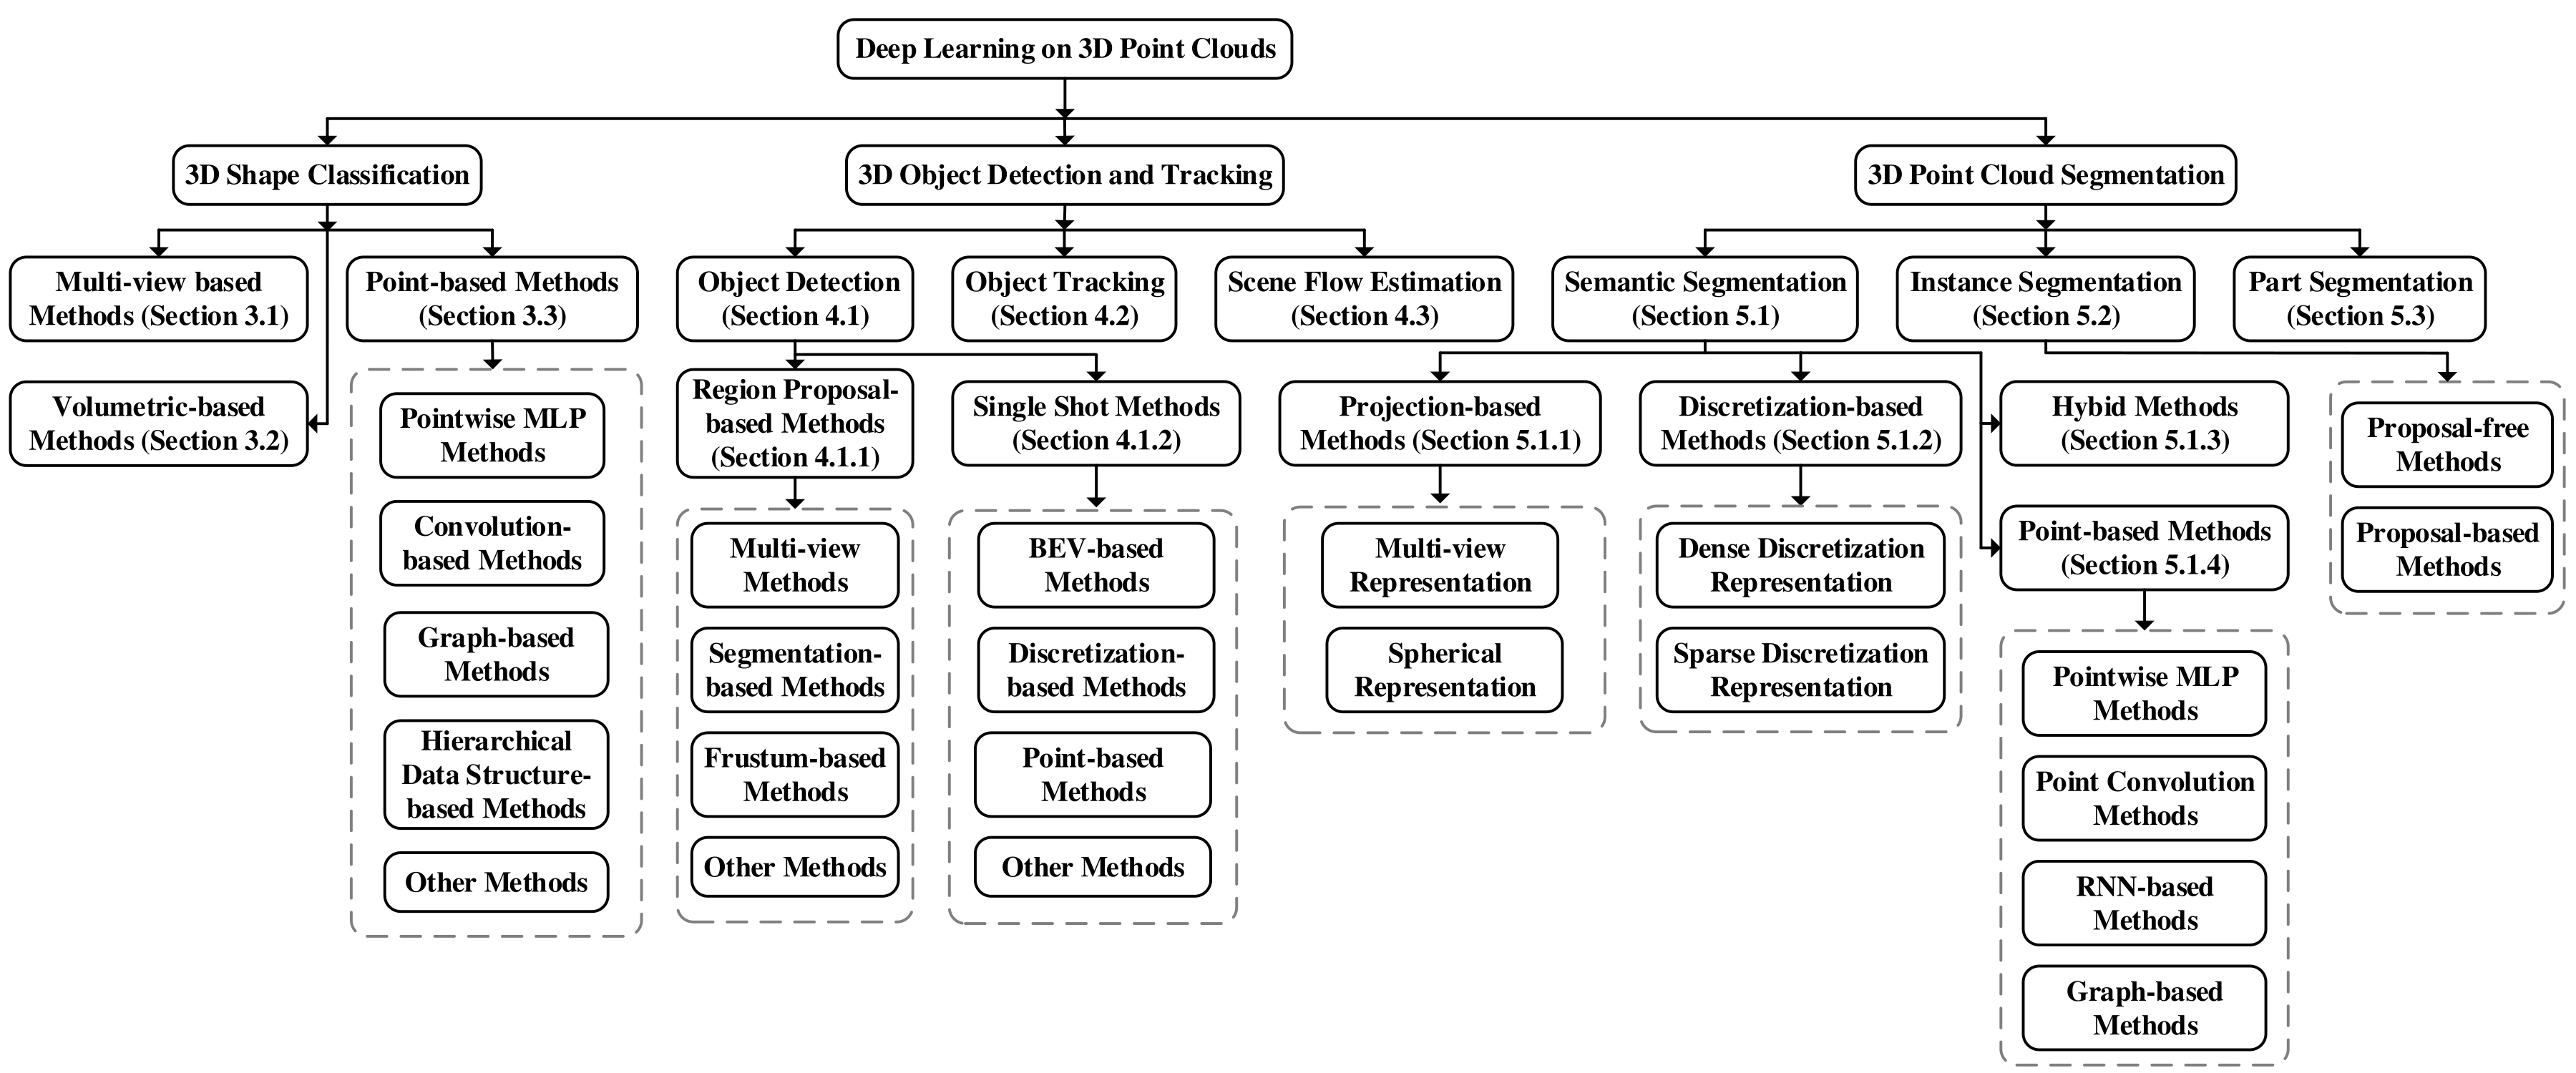
\includegraphics[scale=0.8]{imgs/pointcloud-deeplearning-taxonomy.jpg}
    \caption{A taxonomy of deep learning methods for 3D point clouds.\cite{abs200106280}}
\end{figure}
\noindent
\begin{itemize}
    \item \textbf{3D Shape Classification}: Methods for this task usually learn the embedding of each point first and then extract a global shape embedding from the whole point cloud using an aggregation method. Classification is finally achieved by feeding the global embedding into several fully connected layers. According to the data type of input for neural networks, existing 3D shape classification methods can be divided into \textit{multi-view based}, \textit{volumetric-based} and \textit{point-based} methods.
    \begin{figure}[H]
        \centering
        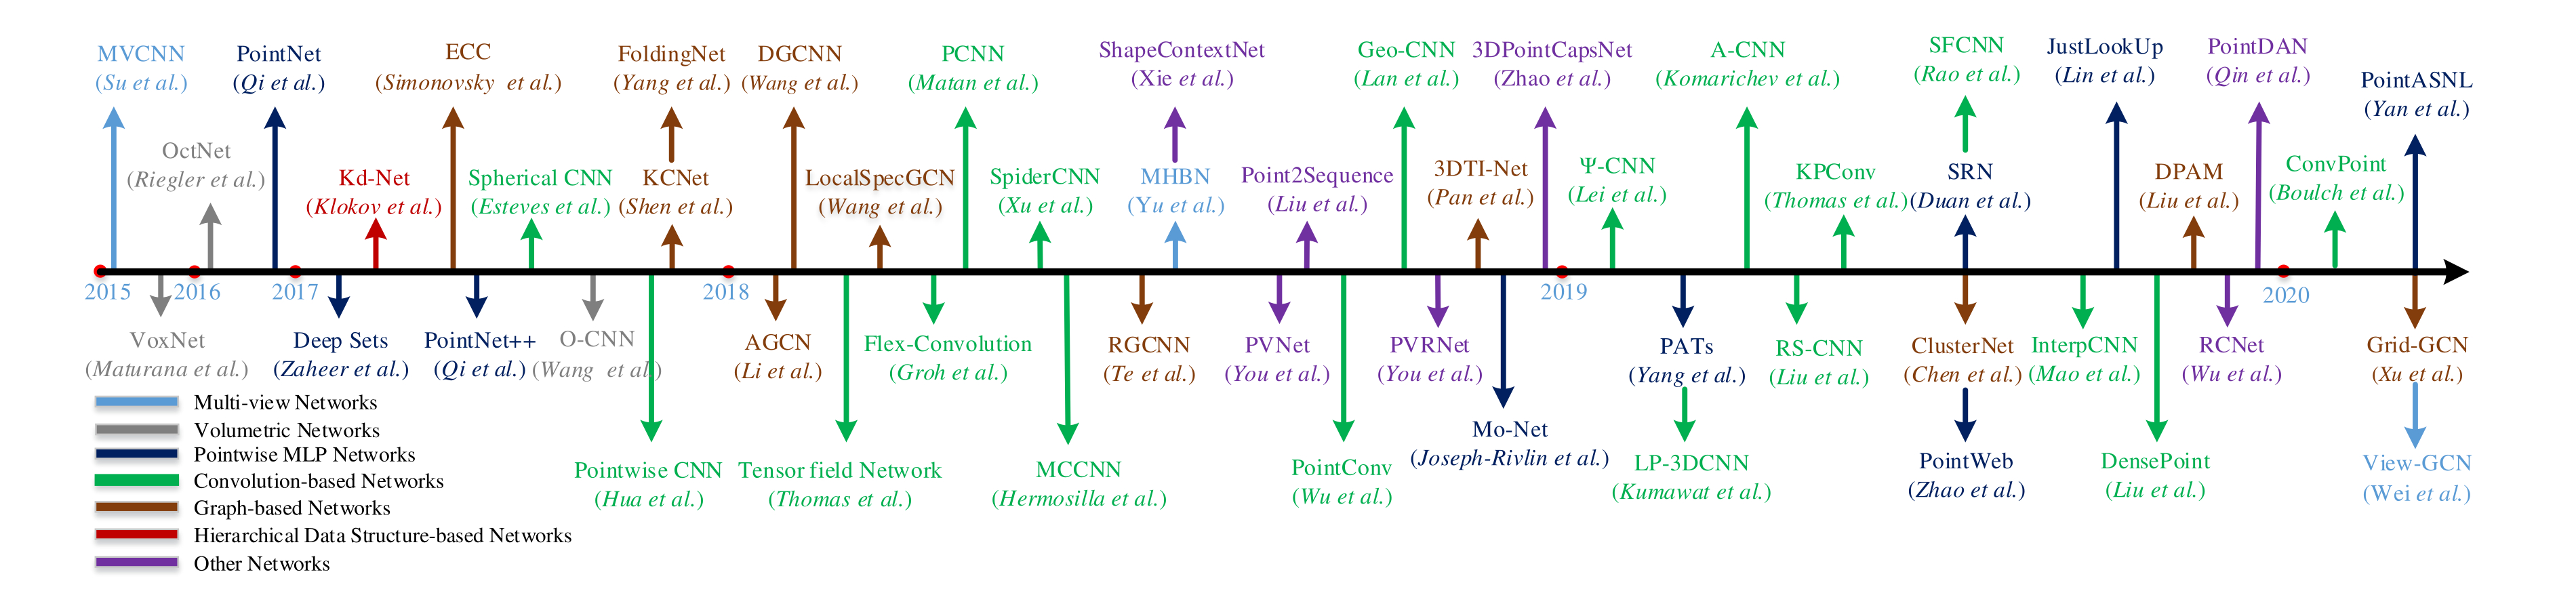
\includegraphics[scale=0.7]{imgs/pointcloud-classification-methods.jpg}
        \caption{Chronological overview of 3D shape classification methods}
    \end{figure}
    \item \textbf{3D Object Detection and Tracking}: A typical 3D object detector takes the point cloud of a scene as its input and produces an oriented 3D bounding box around each detected object. Similar to object detection in images, 3D object detection methods can be divided into two categories: \textit{region proposal-based} and \textit{single shot methods}.
    \begin{figure}[H]
        \centering
        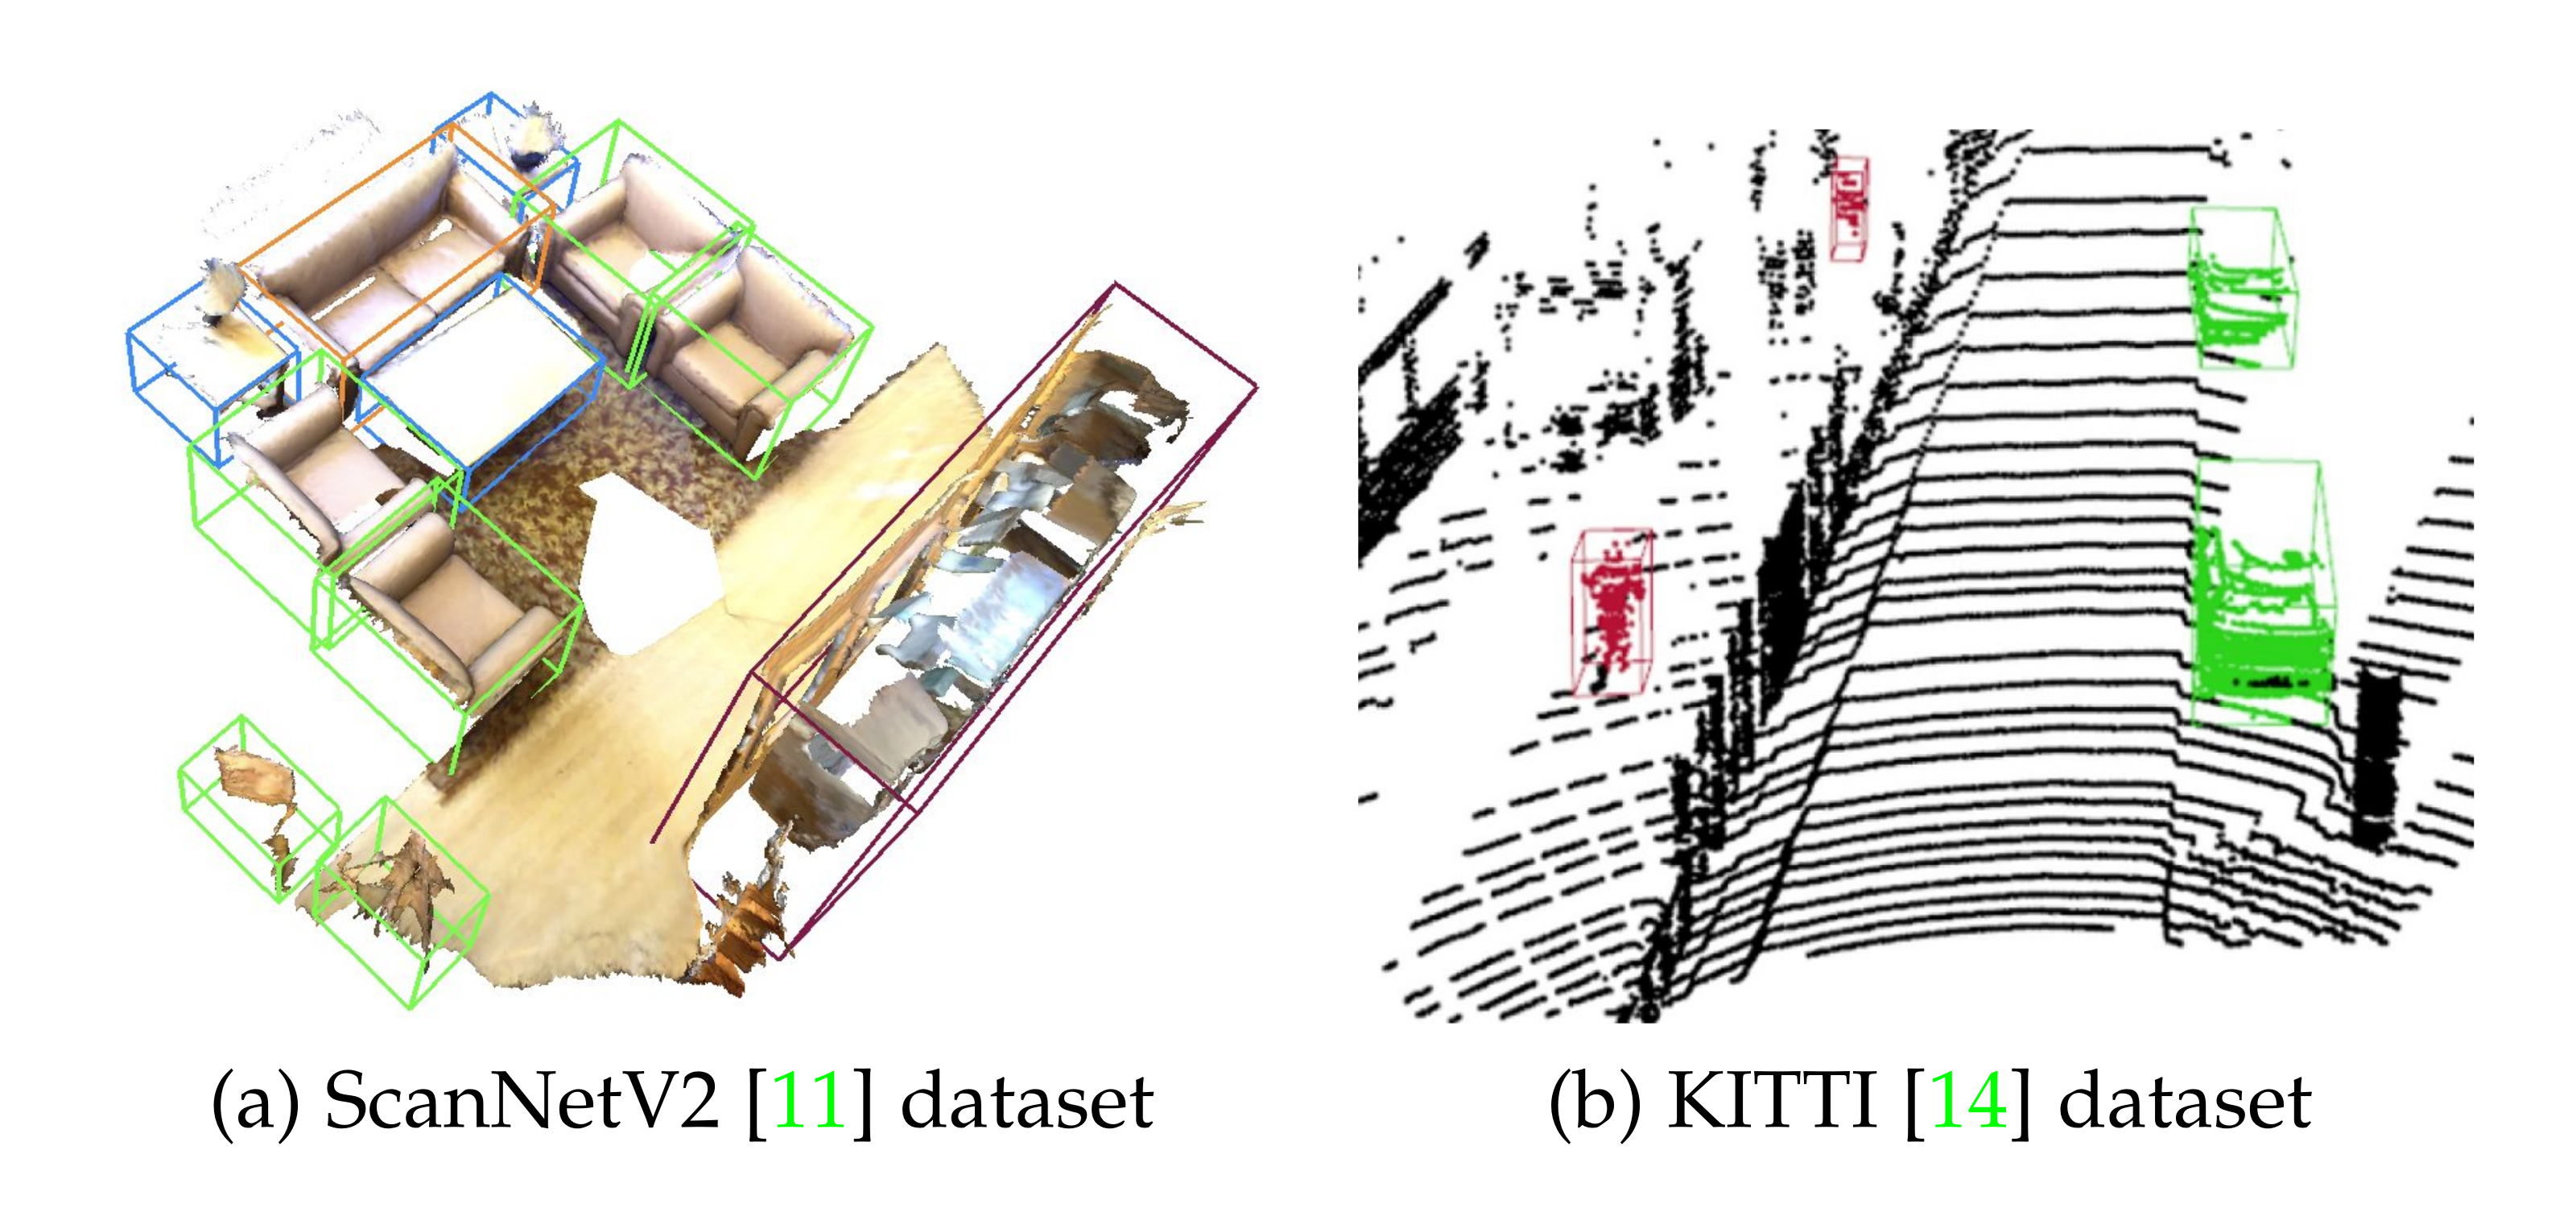
\includegraphics[scale=1.2]{imgs/pointcloud-object-detection.jpg}
    \end{figure}
    \begin{figure}[H]
        \centering
        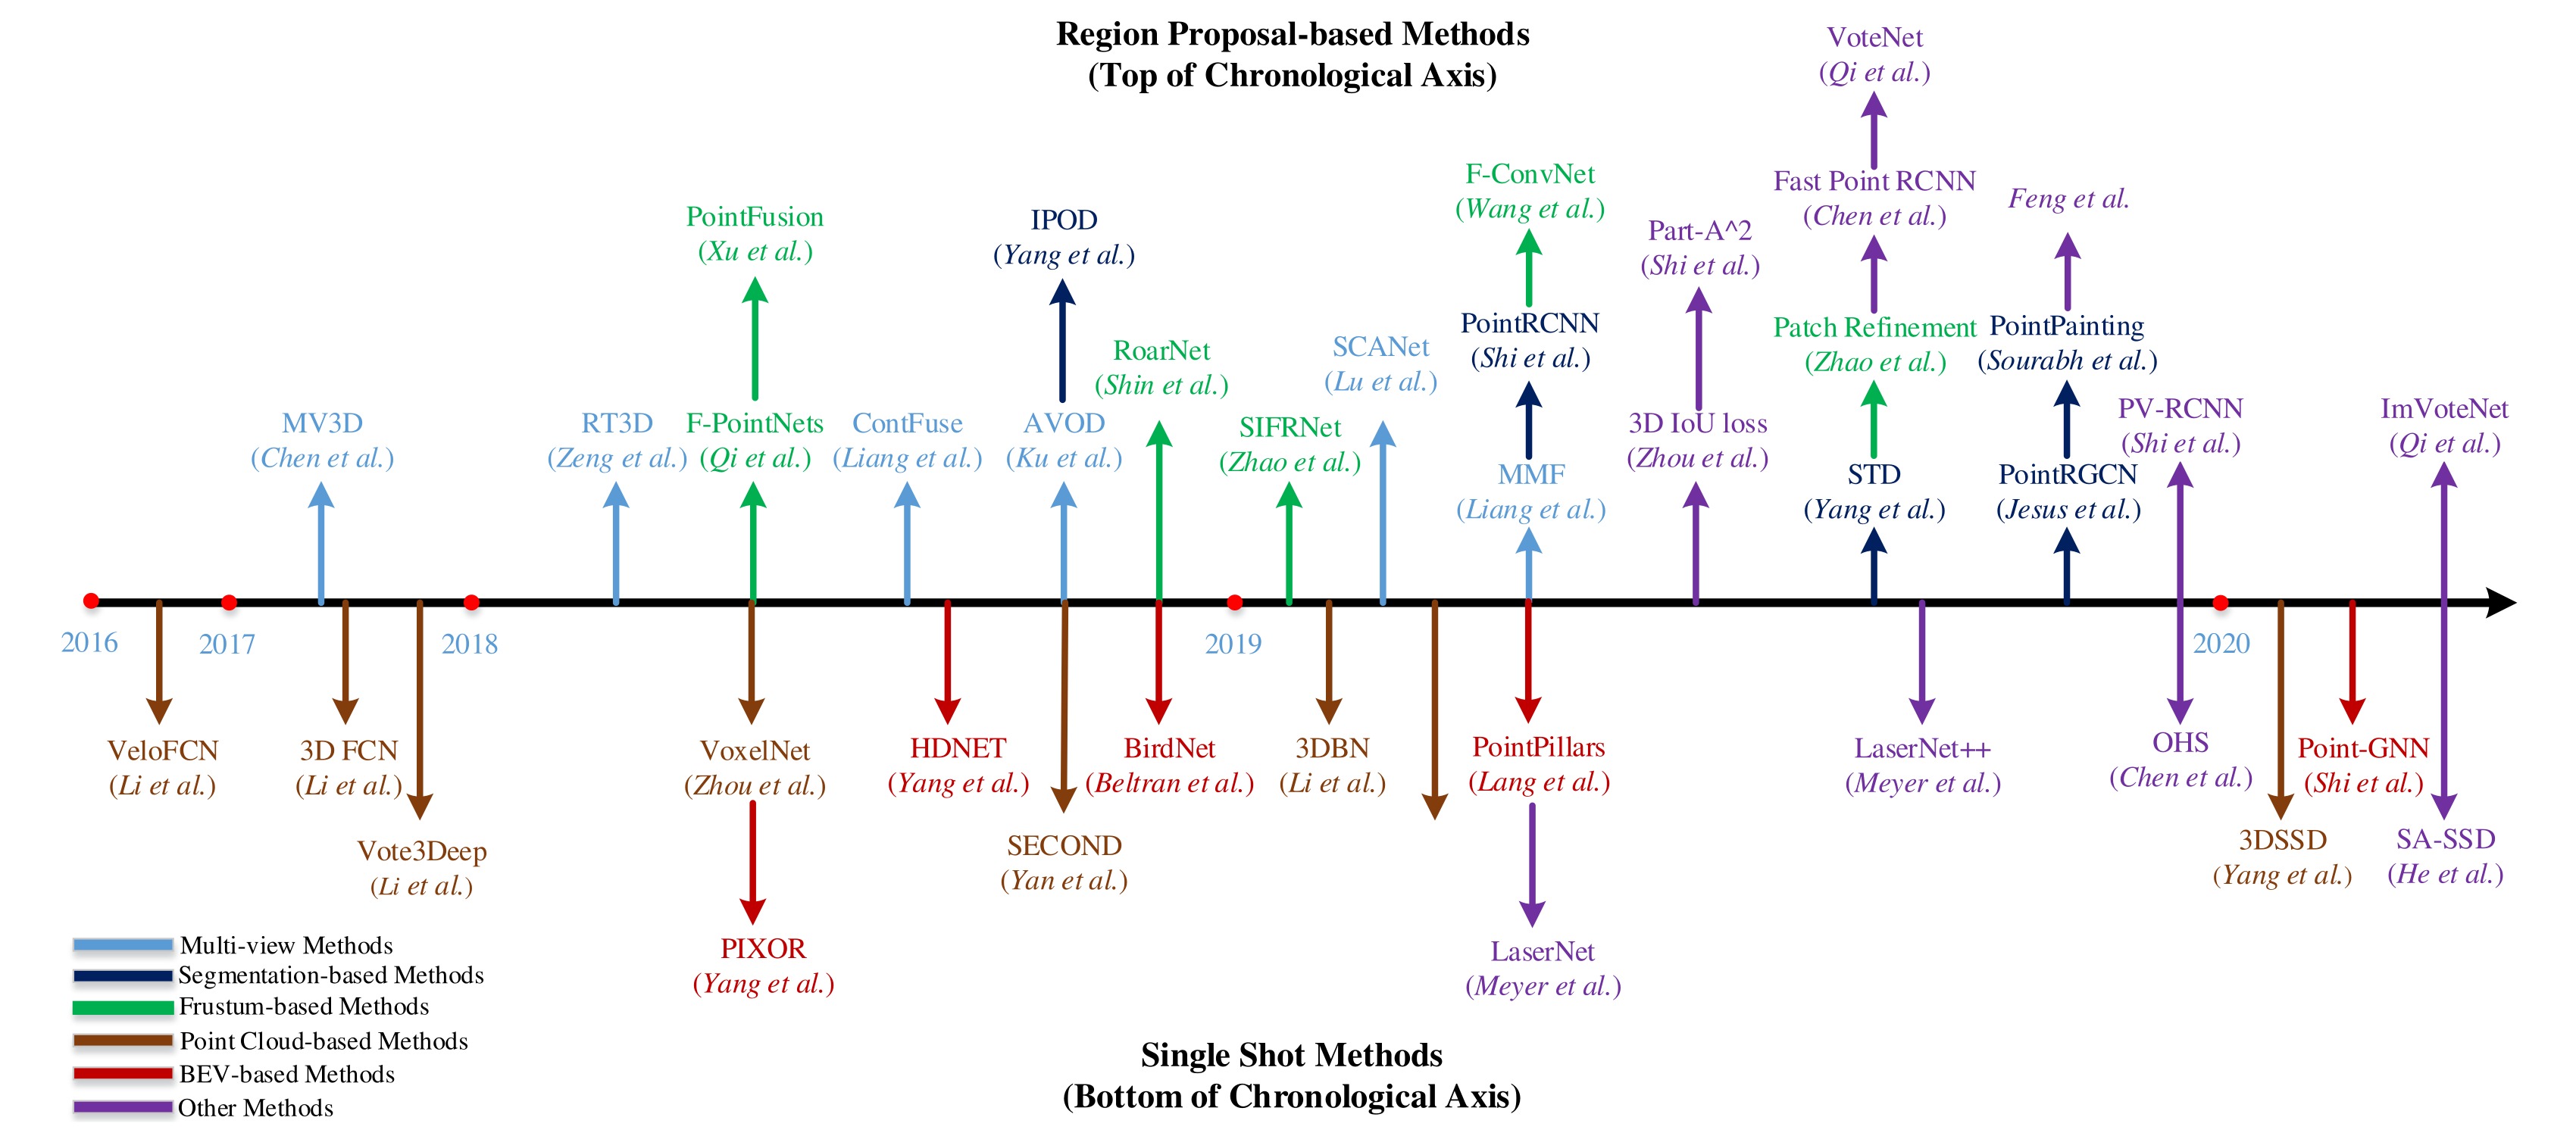
\includegraphics[scale=0.7]{imgs/pointcloud-object-detection-methods.jpg}
        \caption{Chronological overview of 3D object detection methods}
    \end{figure}
    \item \textbf{3D Point Cloud Segmentation}: 3D point cloud segmentation requires the understanding of both the global geometric structure and the fine-grained details of each point. According to the segmentation granularity, 3D point cloud segmentation methods can be classified into three categories: \textit{semantic segmentation} (scene level), \textit{instance segmentation} (object level) and \textit{part segmentation} (part level).
    \begin{figure}[H]
        \centering
        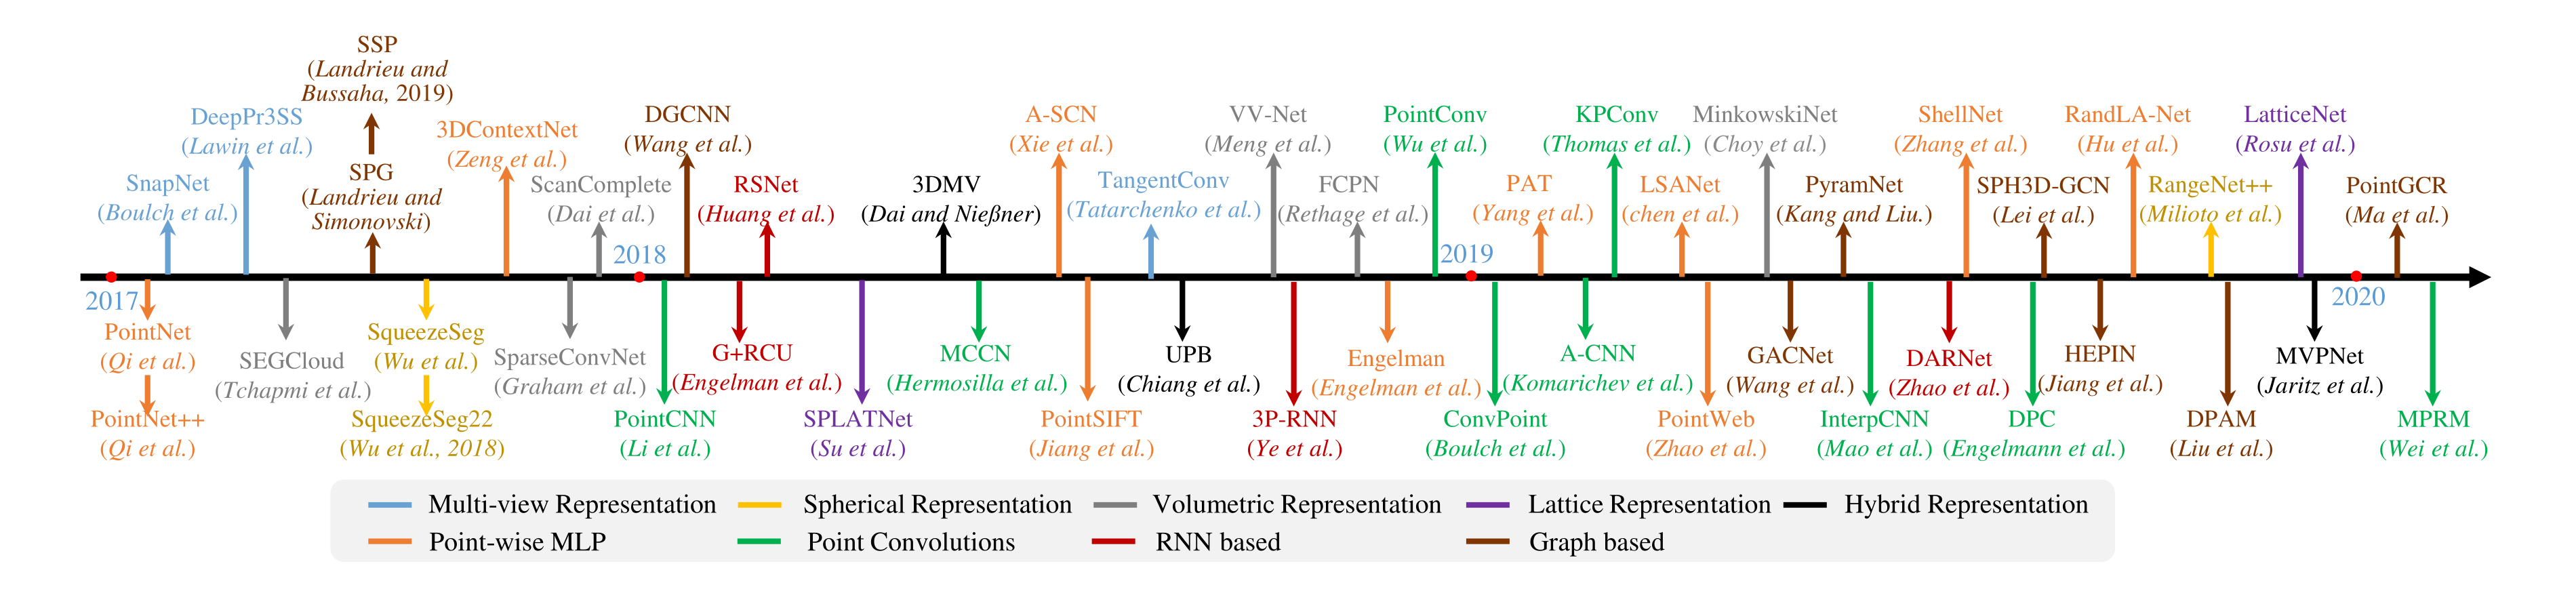
\includegraphics[scale=0.7]{imgs/pointcloud-segmentation-methods.jpg}
        \caption{Chronological overview of 3D semantic segmentation methods}
    \end{figure}
\end{itemize}
\subsection{Challenges of deep learning on point clouds}
Applying deep learning on 3D point cloud data comes with many challenges. Some of these challenges include occlusion which is caused by cluttered scene or blind side; noise/outliers which are unintended points; points misalignment e.t.c. How- ever, the more pronounced challenges when it comes to application of deep learning on point clouds can be categorized into the following:
\begin{figure}[H]
    \centering
    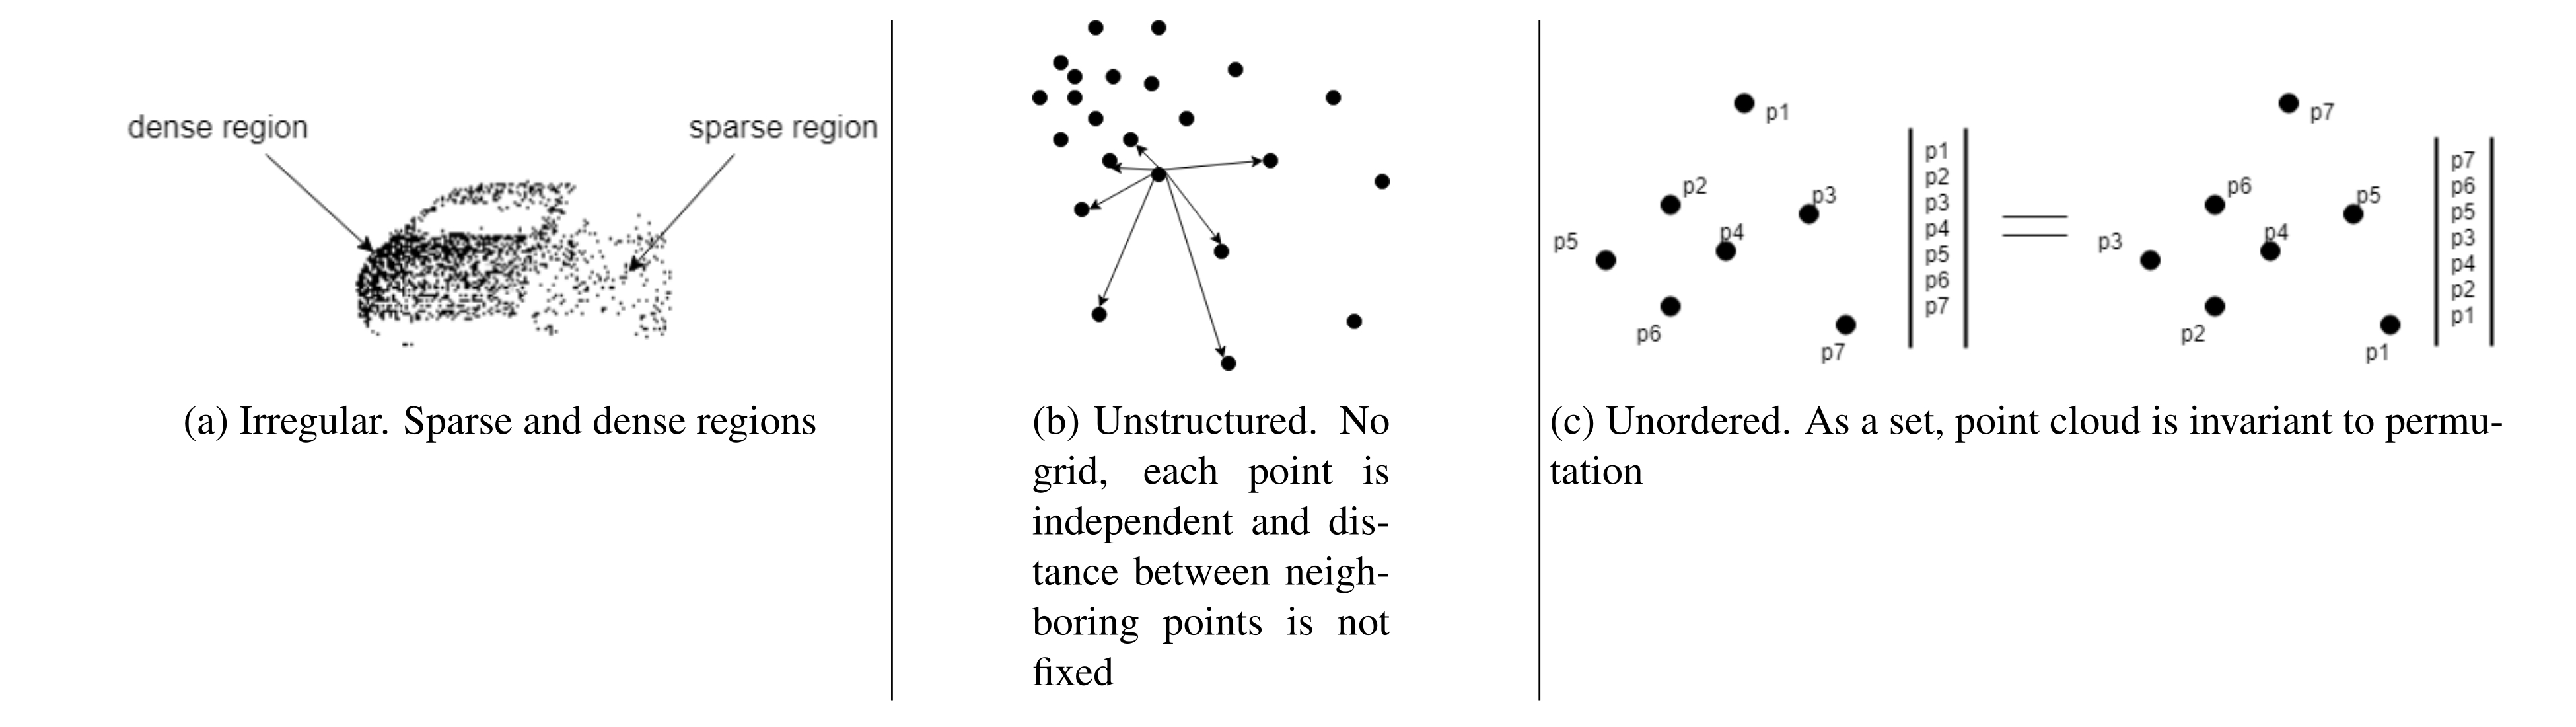
\includegraphics[scale=0.7]{imgs/pointcloud-deeplearning-challenges.jpg}
    \caption{Challenges of deep learning on point clouds}
\end{figure}
\begin{itemize}
    \item \textbf{Irregularity}: point cloud data is irregular, meaning, the points are not evenly sampled accross the different regions of an object/scene, so some regions could have dense points while others sparse points. These can be seen in figure 5a.
    \item \textbf{Unstructured}: point cloud data is not on a regular grid. Each point is scanned independently and its distance to neighboring points is not always fixed, in contrast, pixels in images are represented on a 2-dimension grid, and spacing between two adjacent pixels is always fixed.
    \item \textbf{Unorderdness}: Point cloud of a scene is the set of points (usually represented by $(XYZ)$) obtained around the objects in the scene and are usually stored as a list in a file. As a set, the order in which the points are stored does not change the scene represented. The unordered nature of point sets is shown in figure 5c.
\end{itemize}
These properties of point cloud are very challenging for deep learning, especially convolutional neural networks (CNN). These is because convolutional neural networks are based on convolution operation which is performed on a data that is ordered, regular and on a structured grid. Early approaches overcome these challenges by converting the point cloud into a structured grid format. However, recently researchers have been developing approaches that directly uses the power of deep learning on raw point cloud, taking away the need for preprocessing.

\newpage
\section{Task 1: Dataset Preprocessing}
\label{section:dataset-preprocessing}
The implementation of what is described in this section can be found in the Jupyter Notebook named \texttt{Task1-Preprocessing.ipynb}.\\
\\
For classification, there are two types of datasets: synthetic datasets, and real-world datasets. Objects in the synthetic datasets are complete, without any occlusion and background. In contrast, objects in the real-world datasets are occluded at different levels and some objects are contaminated with background noise. The decision was made to use a synthetic dataset containing 3D models and the correlated rendered images obtained by applying textures. The following random sample is useful to immediately clarify the nature of the data we will be dealing with:
\begin{figure}[H]
    \centering
    \subfloat[\centering 3D Object]{{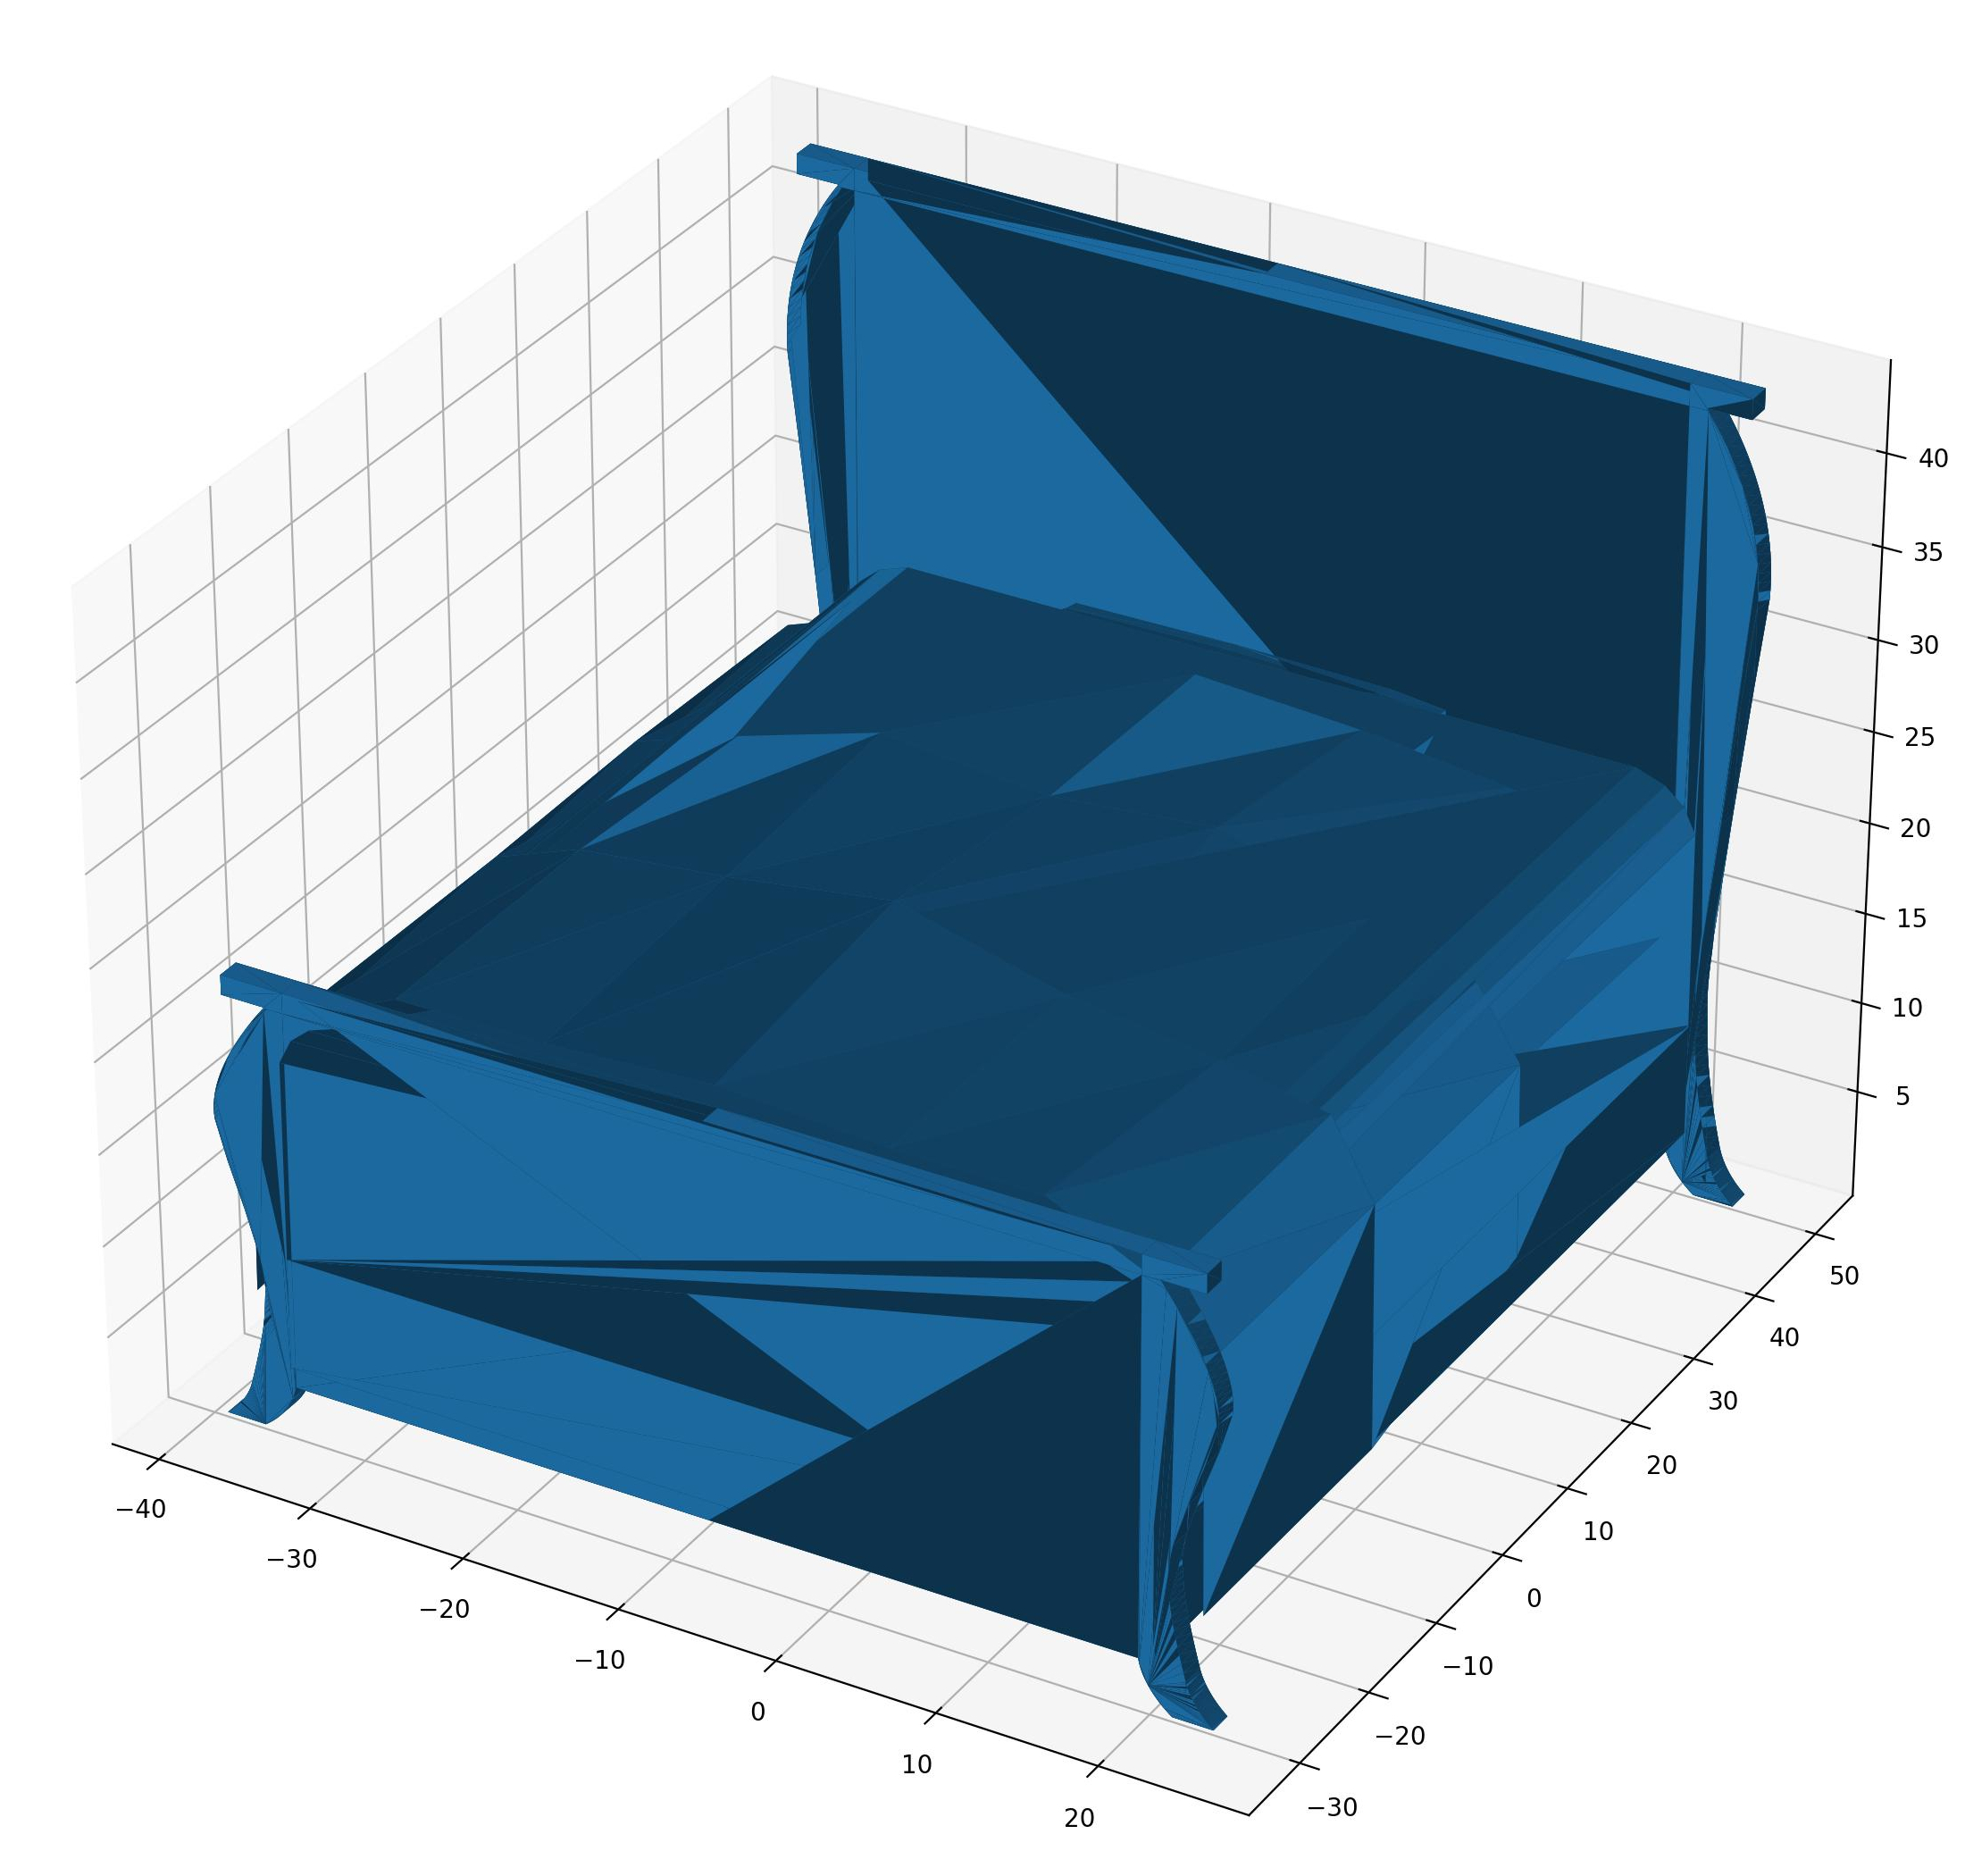
\includegraphics[scale=0.26]{imgs/example-mesh-trisurf.jpg} }}
    \qquad
    \subfloat[\centering Sampled Point Cloud]{{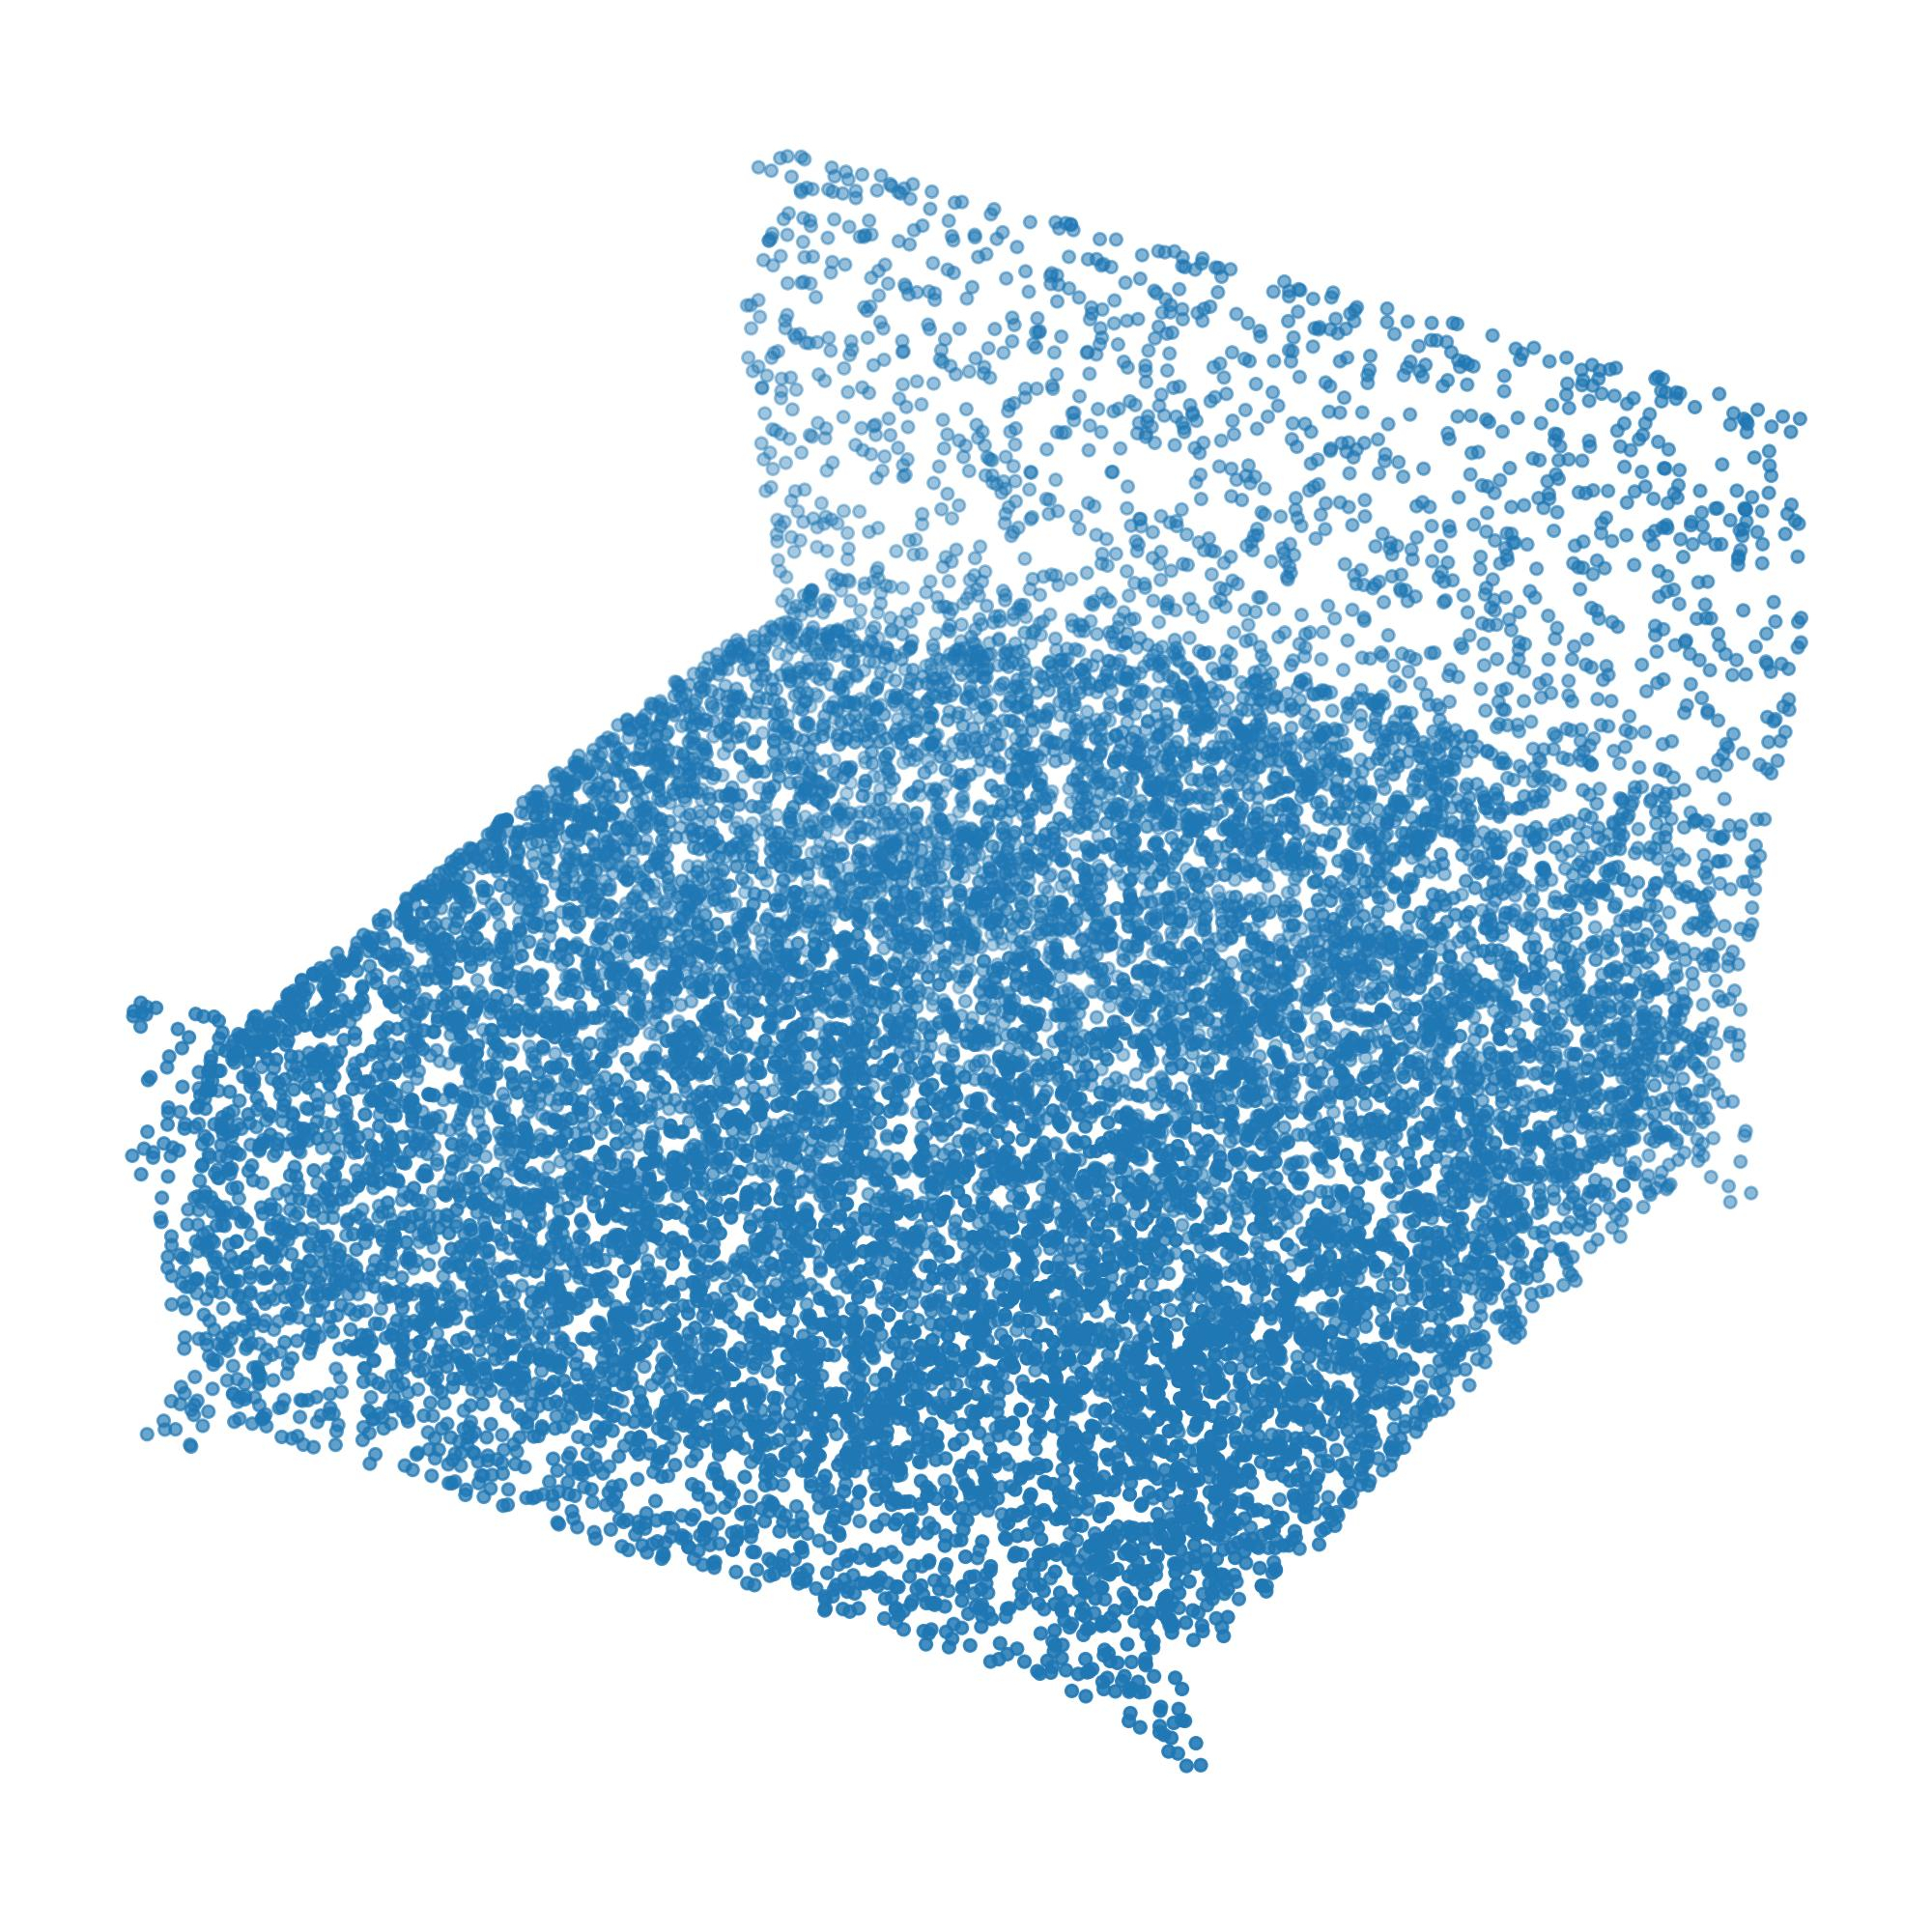
\includegraphics[scale=0.26]{imgs/example-mesh-pointcloud.jpg} }}
    \qquad
    \subfloat[\centering Renders obtained applying textures]{{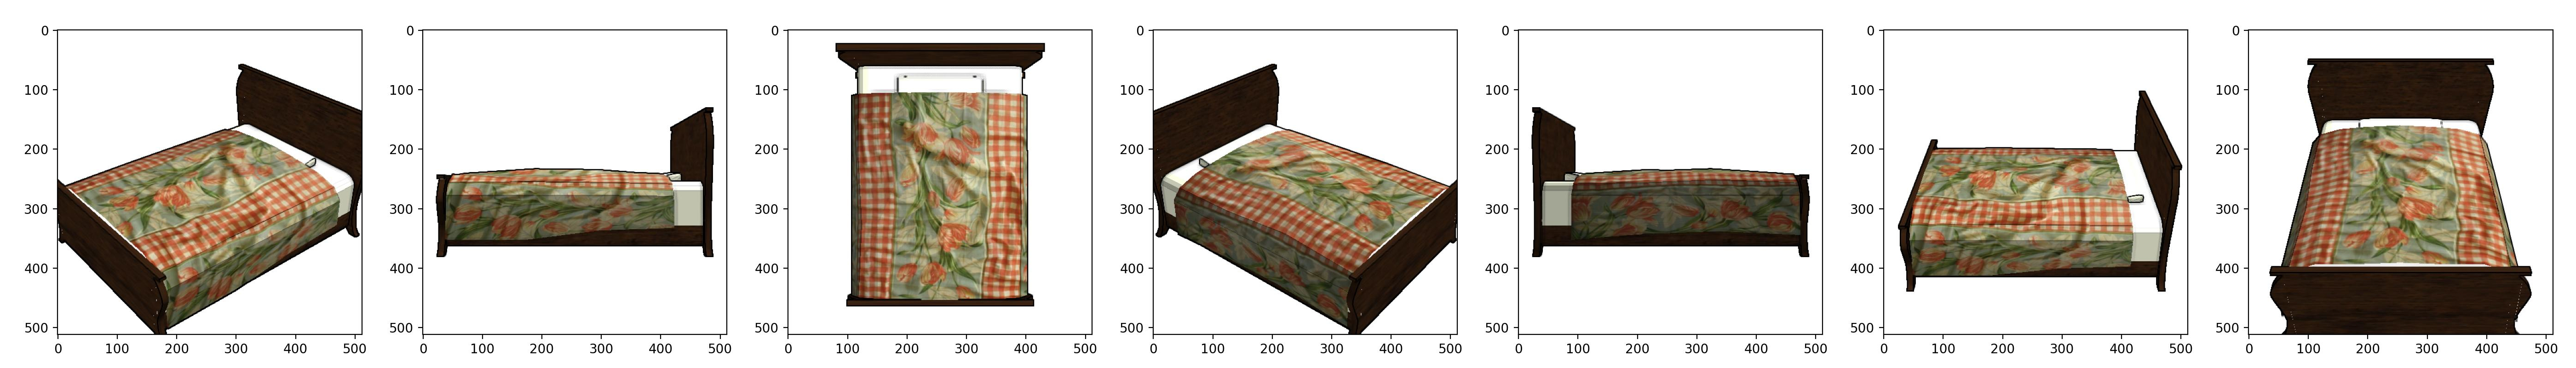
\includegraphics[scale=0.21]{imgs/example-mesh-renders.jpg} }}
    \caption{Random sample from the dataset}
\end{figure}
\subsection{The Dataset: ShapeNet}
ShapeNet\footnote{\url{https://shapenet.org}} is an ongoing effort to establish a richly-annotated, large-scale dataset of 3D shapes. We provide researchers around the world with this data to enable research in computer graphics, computer vision, robotics, and other related disciplines. ShapeNet is a collaborative effort between researchers at Princeton, Stanford and TTIC.
ShapeNet consists of several subsets:
\begin{itemize}
    \item \textbf{ShapeNetCore}: a subset of the full ShapeNet dataset with single clean 3D models and manually verified category and alignment annotations. It covers $55$ common object categories with about $51,300$ unique 3D models. The $12$ object categories of PASCAL 3D+, a popular computer vision 3D benchmark dataset, are all covered by ShapeNetCore.
    \item \textbf{ShapeNetSem} a smaller, more densely annotated subset consisting of $12,000$ models spread over a broader set of $270$ categories. In addition to manually verified category labels and consistent alignments, these models are annotated with real-world dimensions, estimates of their material composition at the category level, and estimates of their total volume and weight.
\end{itemize}
\textbf{The project was developed using ShapeNetSem for the following reasons:}
\begin{itemize}
    \item it includes pre-rendered screenshots of each model from 6 canonical orientations (front, back, left, right, bottom, top), and another 6 "turn table" positions around the model;
    \item the included \texttt{metadata.csv} file provides metadata with class labels associated with each model\footnote{Each model in ShapeNet is linked to an appropriate synset in WordNet: WordNet is a large lexical database of English. Nouns, verbs, adjectives and adverbs are grouped into sets of cognitive synonyms (synsets), each expressing a distinct concept (\url{https://wordnet.princeton.edu}).};
    \item each object is identified by means of a unique hexadecimal string\\(i.e. \texttt{100f39dce7690f59efb94709f30ce0d2});
\end{itemize}
Due to size limitations I did not provide the dataset included in the shared Google drive. To get access to it, I made a request using University of Pisa education email address. The following credentials can be used to \textbf{directly download} the dataset from the ShapeNet organization website\footnote{\url{https://shapenet.org}}:
\begin{lstlisting}[language=bash,frame=single]
Username: rambodrahmani
Password: Cnk4mBZ77Z5Av6v
\end{lstlisting}
Some preliminary preprocessing tasks were performed as detailed in the following subsections.
\subsection{Merge 3D models and renders}
In the original dataset, 3D models \texttt{.obj} files and rendered \texttt{.png} files are provided in separate \texttt{.zip} archives.
\begin{lstlisting}[language=bash]
$ tree ShapeNetSem-models
\end{lstlisting}
\dirtree{%
.1 ShapeNetSem-models.
.2 1004f30be305f33d28a1548e344f0e2e.mtl.
.2 1004f30be305f33d28a1548e344f0e2e.obj.
.2 100f39dce7690f59efb94709f30ce0d2.mtl.
.2 100f39dce7690f59efb94709f30ce0d2.obj.
.2 101354f9d8dede686f7b08d9de913afe.mtl.
.2 101354f9d8dede686f7b08d9de913afe.obj.
.2 ....
}
\begin{lstlisting}[language=bash]
$ tree ShapeNetSem-renders
\end{lstlisting}
\dirtree{%
.1 ShapeNetSem-models.
.2 1004f30be305f33d28a1548e344f0e2e.
.3 1004f30be305f33d28a1548e344f0e2e-0.png.
.3 1004f30be305f33d28a1548e344f0e2e-1.png.
.3 ....
.2 100f39dce7690f59efb94709f30ce0d2.
.3 100f39dce7690f59efb94709f30ce0d2-0.png.
.3 100f39dce7690f59efb94709f30ce0d2-1.png.
.3 ....
.2 ....
}
\noindent
The first preprocessing task consisted in merging this two archives to have all the raw data in a single directory. During this process, only \texttt{.obj} and \texttt{.png} files were maintained since \texttt{.mtl} files are of no use for our purposes. The resulting preliminary structure of the dataset is the following:
\begin{lstlisting}[language=bash]
$ tree ShapeNetSem-renders
\end{lstlisting}
\dirtree{%
.1 ShapeNetSem-models.
.2 1004f30be305f33d28a1548e344f0e2e.
.3 1004f30be305f33d28a1548e344f0e2e.obj.
.3 1004f30be305f33d28a1548e344f0e2e-0.png.
.3 1004f30be305f33d28a1548e344f0e2e-1.png.
.3 ....
.2 100f39dce7690f59efb94709f30ce0d2.
.3 100f39dce7690f59efb94709f30ce0d2.obj.
.3 100f39dce7690f59efb94709f30ce0d2-0.png.
.3 100f39dce7690f59efb94709f30ce0d2-1.png.
.3 ....
.2 ....
}
\noindent
\subsection{Organize data in macro-categories}
In the original dataset, models are divided in $270$ categories. I decided to aggregate them in $20$ macro-categories in order to:
\begin{itemize}
    \item have a higher number of samples for each category;
    \item make the classification task more comprehensible;
\end{itemize}
In order to achieve this result, the \texttt{metadata.csv} file was used.
\begin{figure}[H]
    \centering
    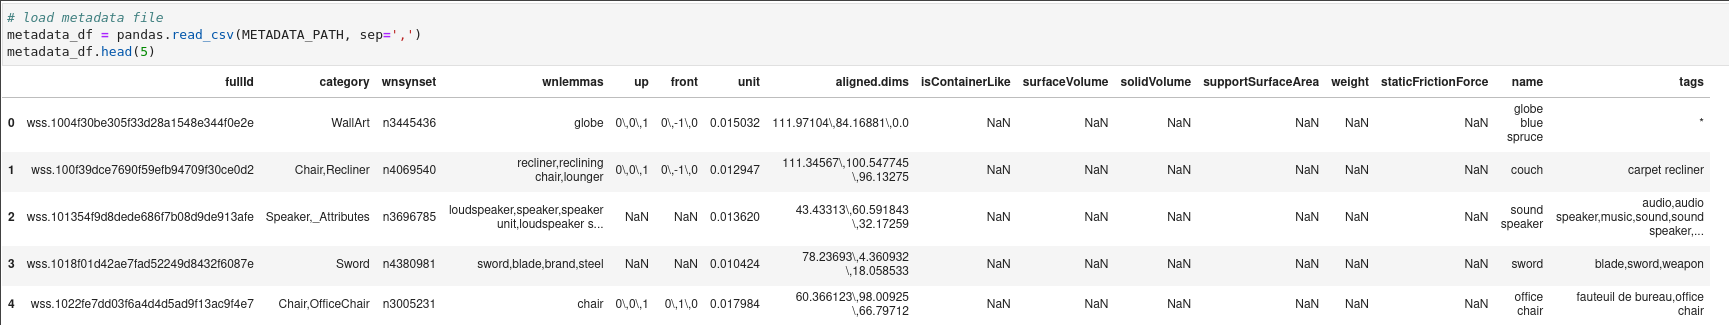
\includegraphics[scale=0.24]{imgs/metadata-pandas-df.png}
    \caption{Metadata \texttt{.csv} file loaded as \texttt{pandas} dataframe}
\end{figure}
\noindent
It provides the following information for each of the models:
\begin{itemize}
    \item \textbf{ID:} hexadecimal string used to uniquely identify each model in the ShapeNet dataset;
    \item \textbf{category:} object class label;
    \item \textbf{wnsynset:} identifies the associated synset in WordNet; the synset is a set of one or more synonyms that are interchangeable in some context without changing the truth value of the proposition in which they are embedded;
    \item \textbf{wnlemmas:} one or more lemmas associated to the given synset ID in WordNet; a lemma represents a specific sense of a specific word;
    \item \textbf{name:} object name;
    \item \textbf{tags:} additional tags associated with the object class label;
\end{itemize}
The following snippet extract from \texttt{metadata.csv} clarifies it better with examples:\\
\\
\setlength\extrarowheight{5pt}
\rowcolors{2}{gray!25}{white}
\begin{tabular}{|p{2cm}|p{2cm}|p{3.2cm}|p{2cm}|p{3.2cm}|p{3cm}}
\rowcolor{gray!50}
\hline
category & wnsynset & wnlemmas & name & tags\\
\hline
Chair, Recliner & n4069540 & recliner, reclining chair, lounger & couch & carpet recliner\\
\hline
Chair, OfficeChair & n3005231 & chair & office chair & fauteuil de bureau, office chair\\
\hline
Computer, Desktop & n3184677 & desktop computer & alienware & computer case pc\\
\hline
Plant & n17402 & plant, flora, plant, life & rose & flower, nature, petal, red, rose\\
\hline
\end{tabular}\\
\\
The possible values of the \texttt{category} field were reduced from $270$ to $20$ relaying on the information provided by other columns such as \texttt{wnsynset}, \texttt{wnlemmas}, \texttt{name} and \texttt{tags}.\\
\\
To conclude, putting it all together, for each object in the dataset we have the following information:
\begin{figure}[H]
    \centering
    \subfloat[\centering 3D Object]{{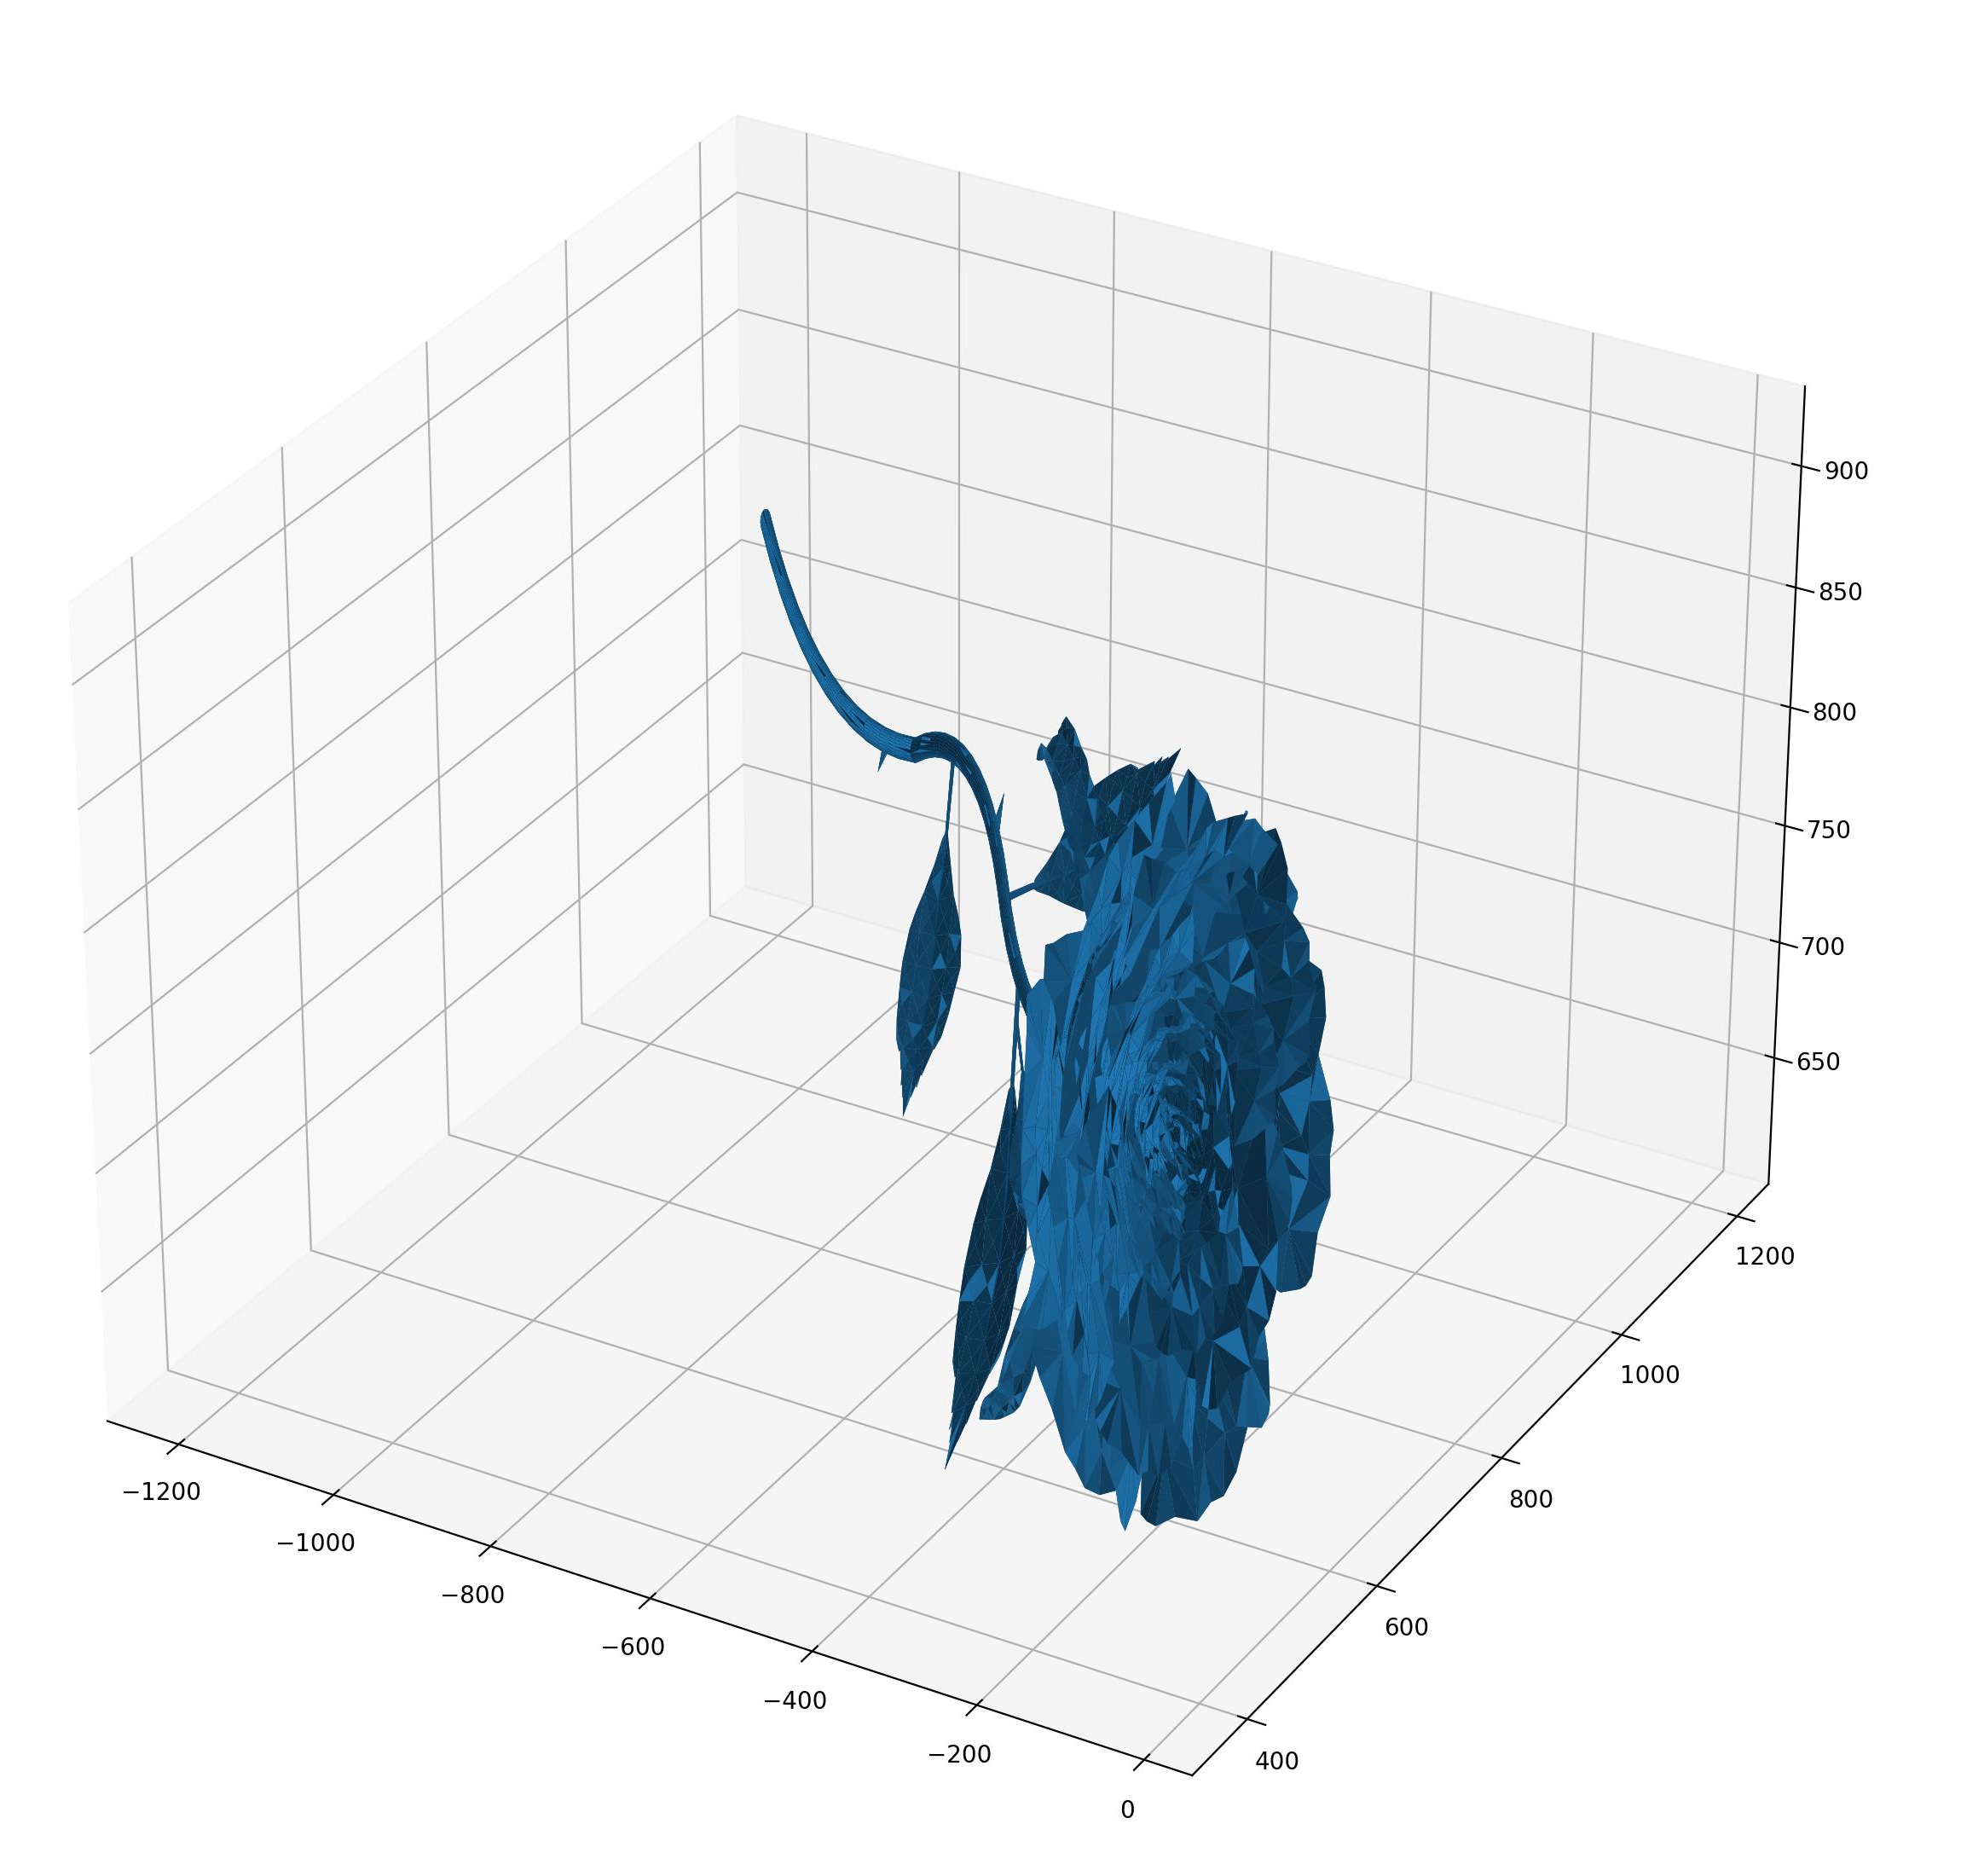
\includegraphics[scale=0.30]{imgs/example-mesh-2-trisurf.jpg} }}
    \qquad
    \subfloat[\centering Sampled Point Cloud]{{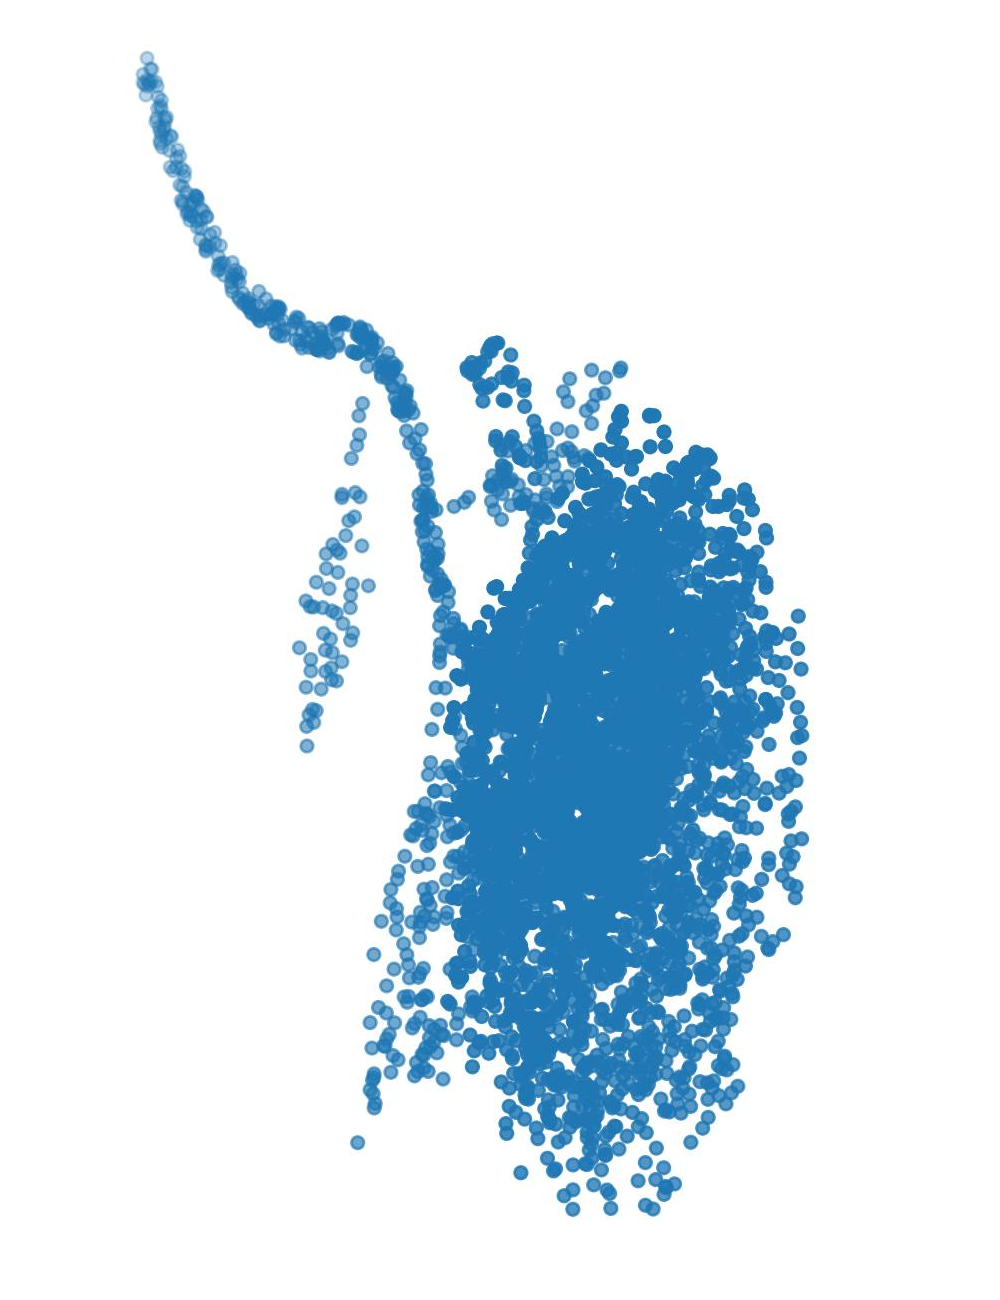
\includegraphics[scale=0.40]{imgs/example-mesh-2-pointcloud.jpg} }}
\end{figure}
\begin{figure}[H]
    \centering
    \subfloat[\centering Renders obtained applying textures]{{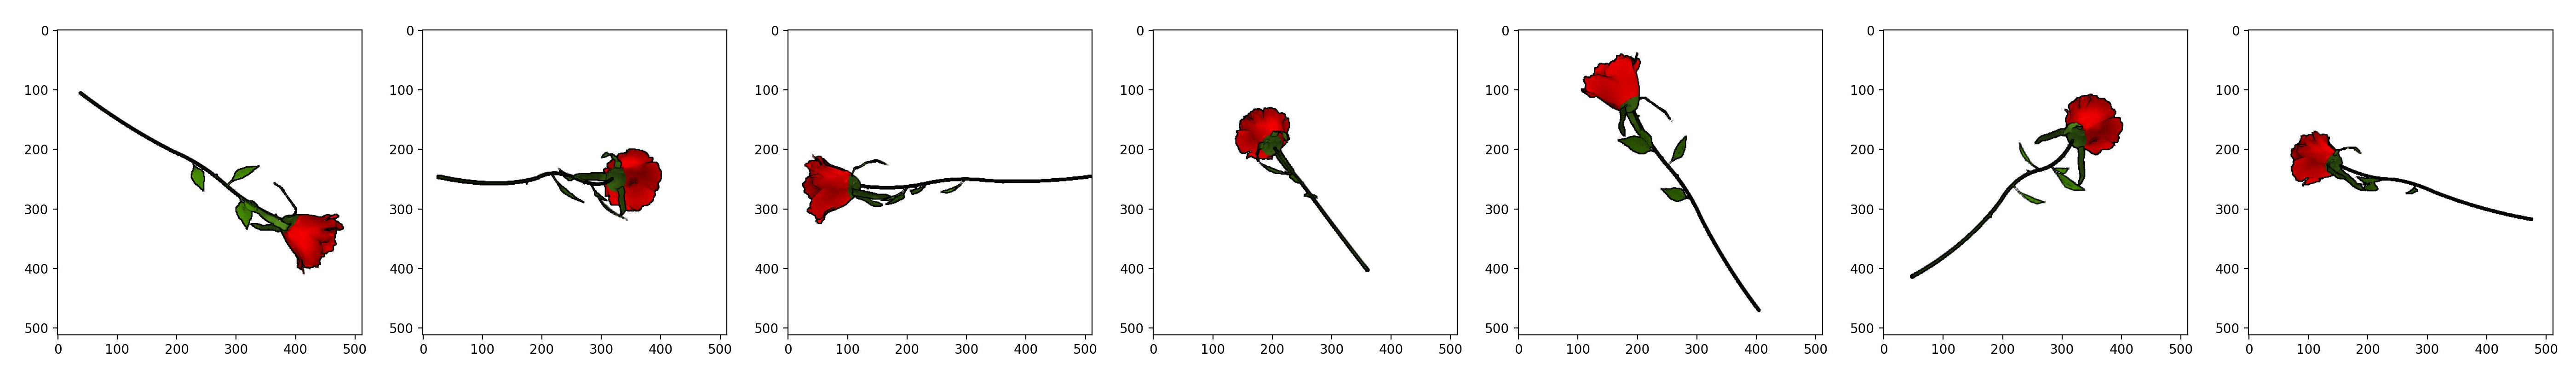
\includegraphics[scale=0.21]{imgs/example-mesh-2-renders.jpg} }}
\end{figure}
\begin{lstlisting}[language=bash,frame=single,caption={Random sample from the dataset},captionpos=b]
FullID: wss.1043b403dd2e79128081f4adb71040
Category: Plant
WNsynset: n17402
WNlemmas: plant, flora, plant life
Name: rose
Tags: boy, flower, girl, landscape, love, nature, petal, plant, red
\end{lstlisting}
After aggregating the initial $270$ categories, the following macro-categories were identified:
\begin{figure}[H]
    \centering
    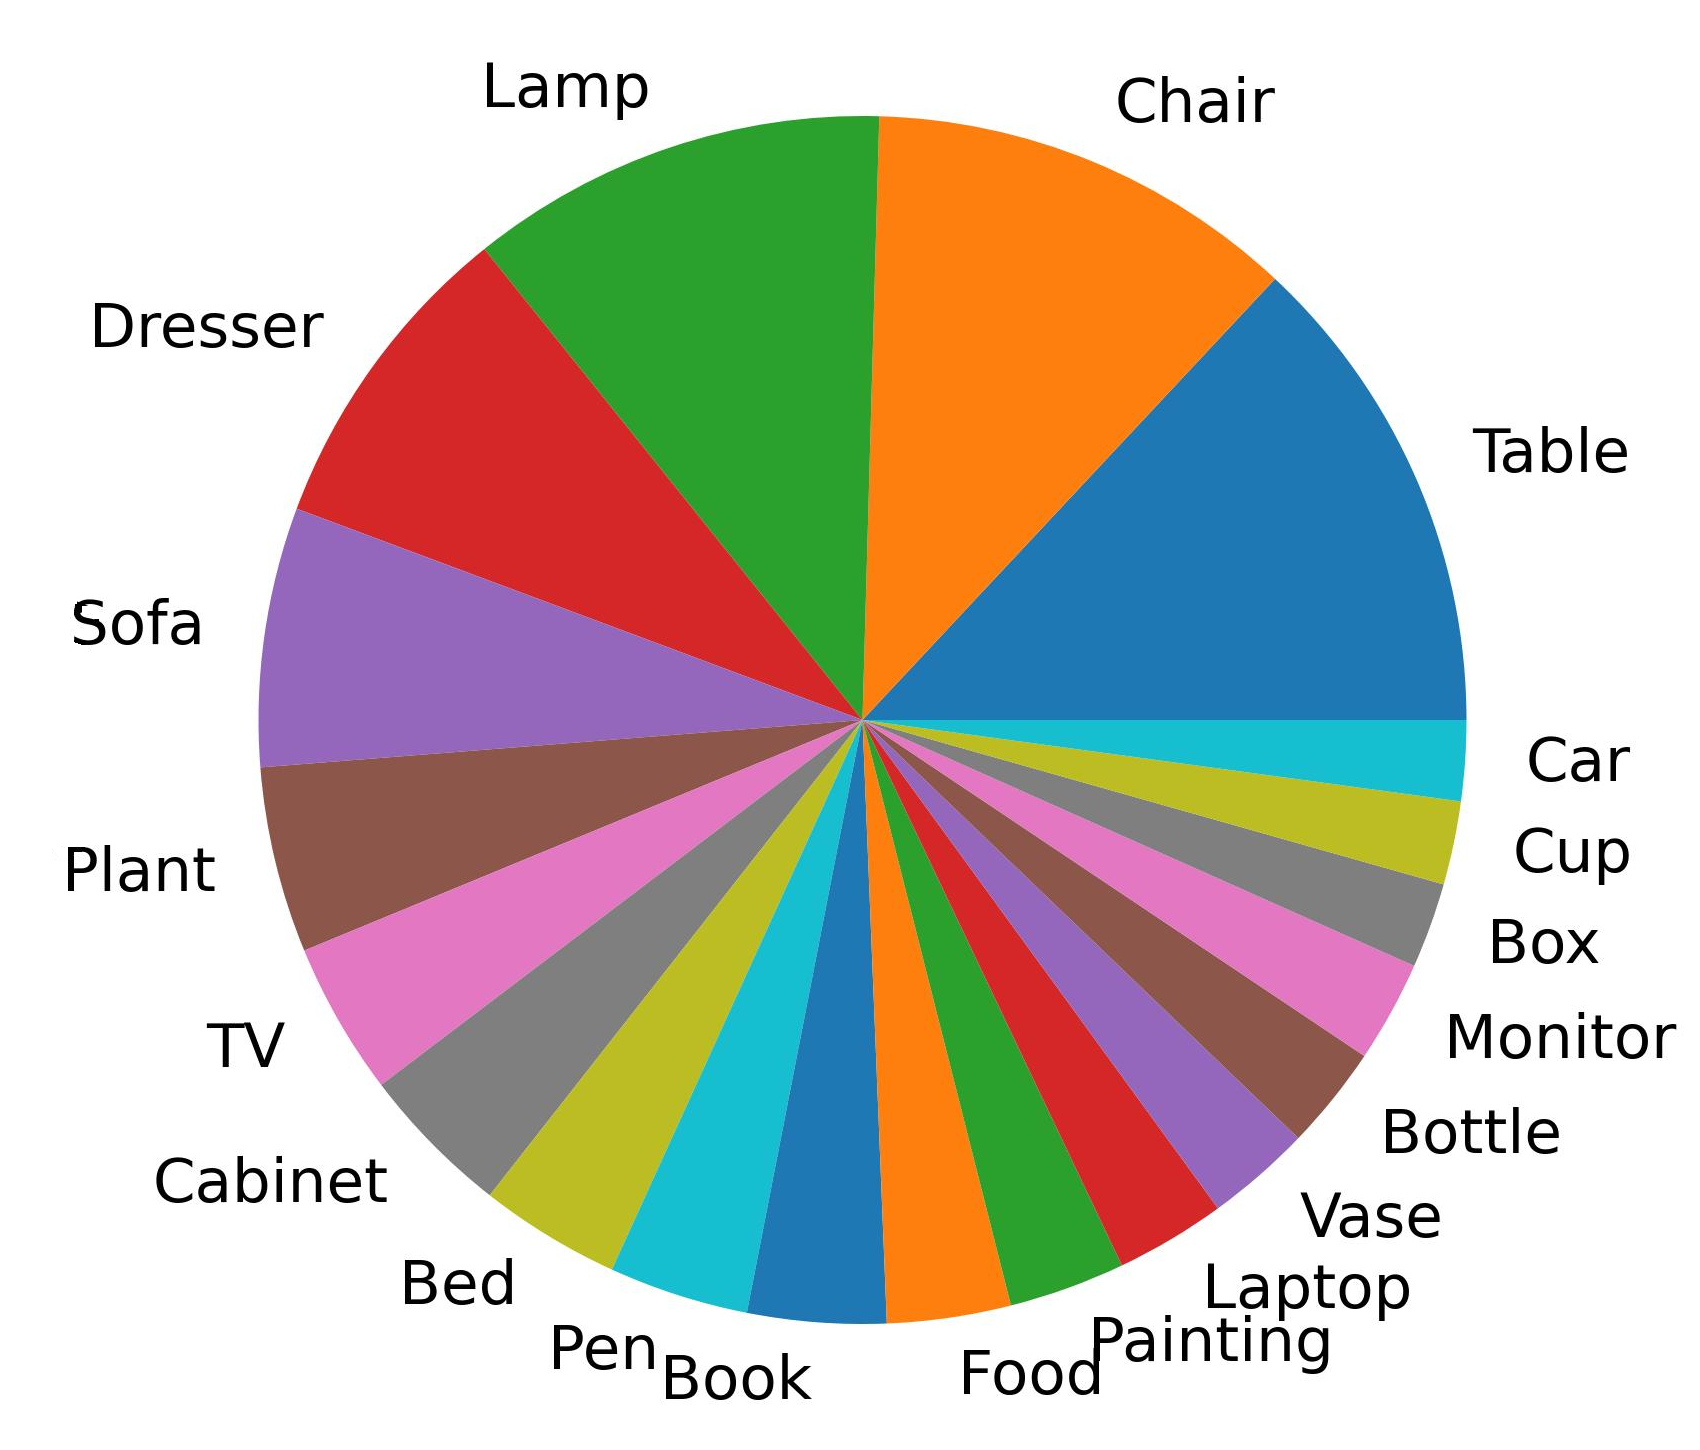
\includegraphics[scale=0.50]{imgs/macro-categories.jpg}
    \caption{Macro-categories}
\end{figure}
\subsection{Dataset balancing}
As it can be seen from the following bar charts, the dataset is not balanced. In addition, the quantity of images samples is higher than the one of 3D pointclouds; this is understandable since for each 3D model 12 pre-rendered screenshots are provided.
\begin{figure}[H]
    \centering
    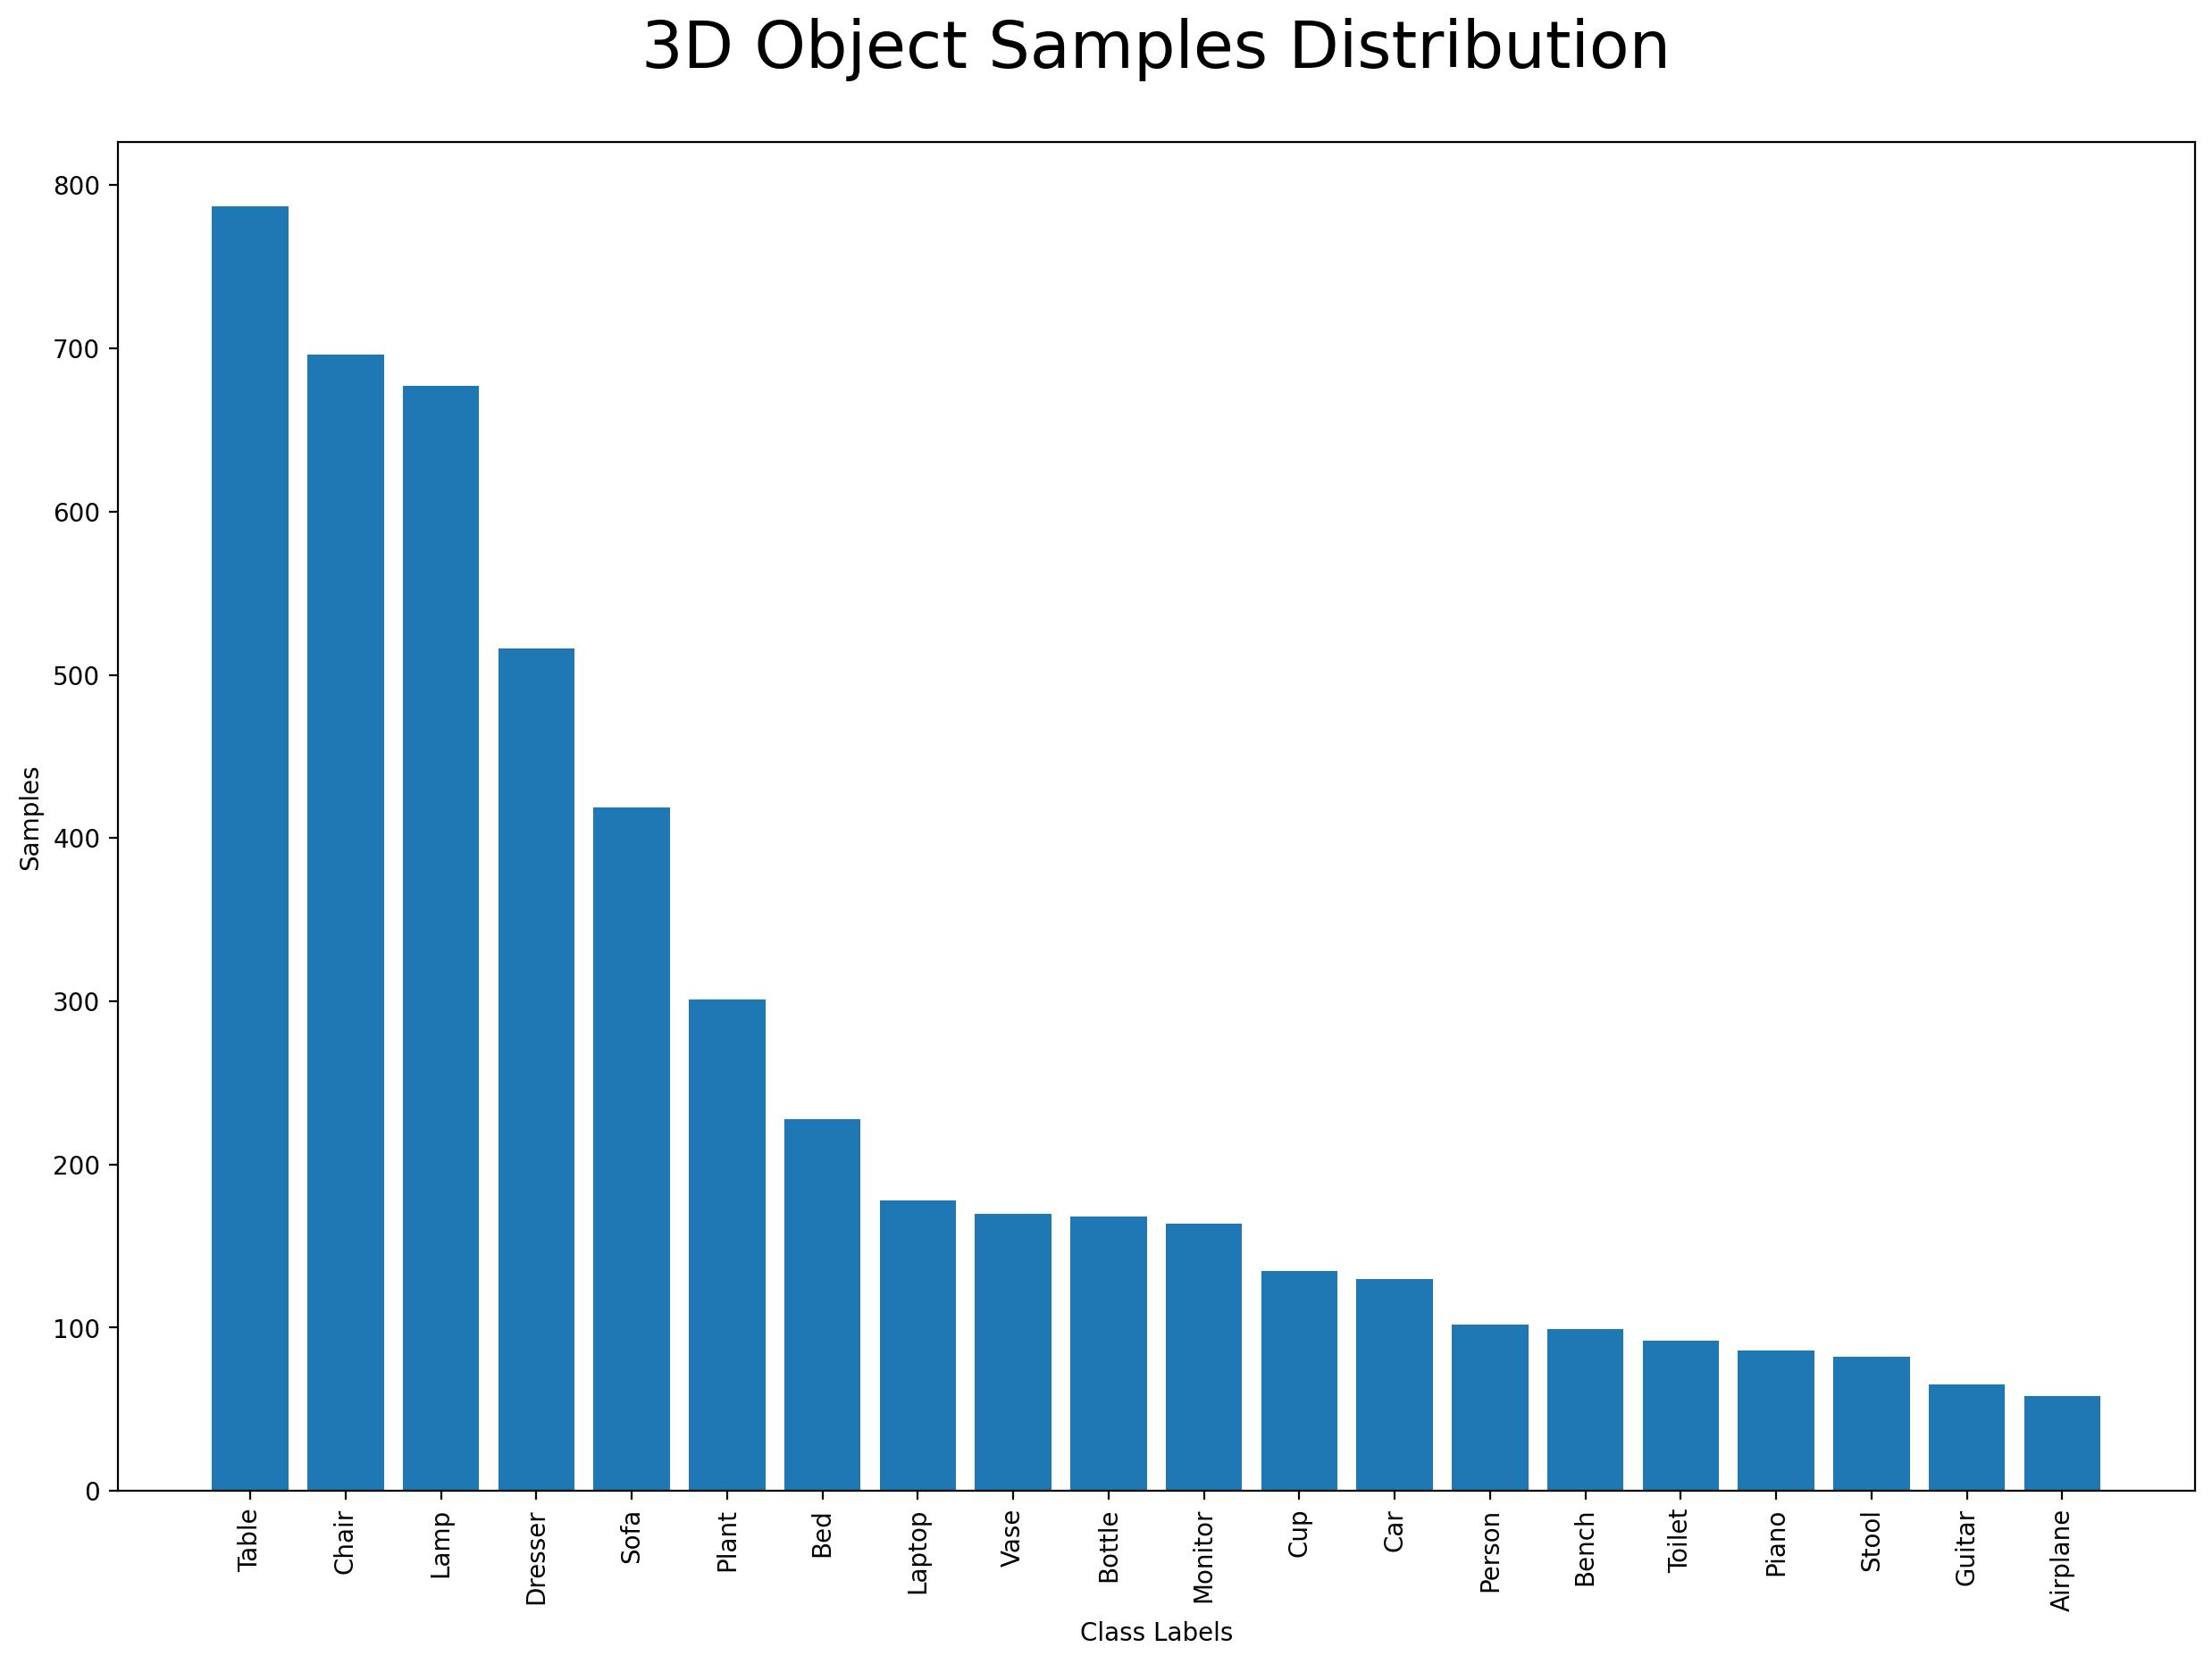
\includegraphics[scale=0.35]{imgs/3d-object-samples-distribution.jpg}
    \caption{3D Object Samples per class}
\end{figure}
\begin{figure}[H]
    \centering
    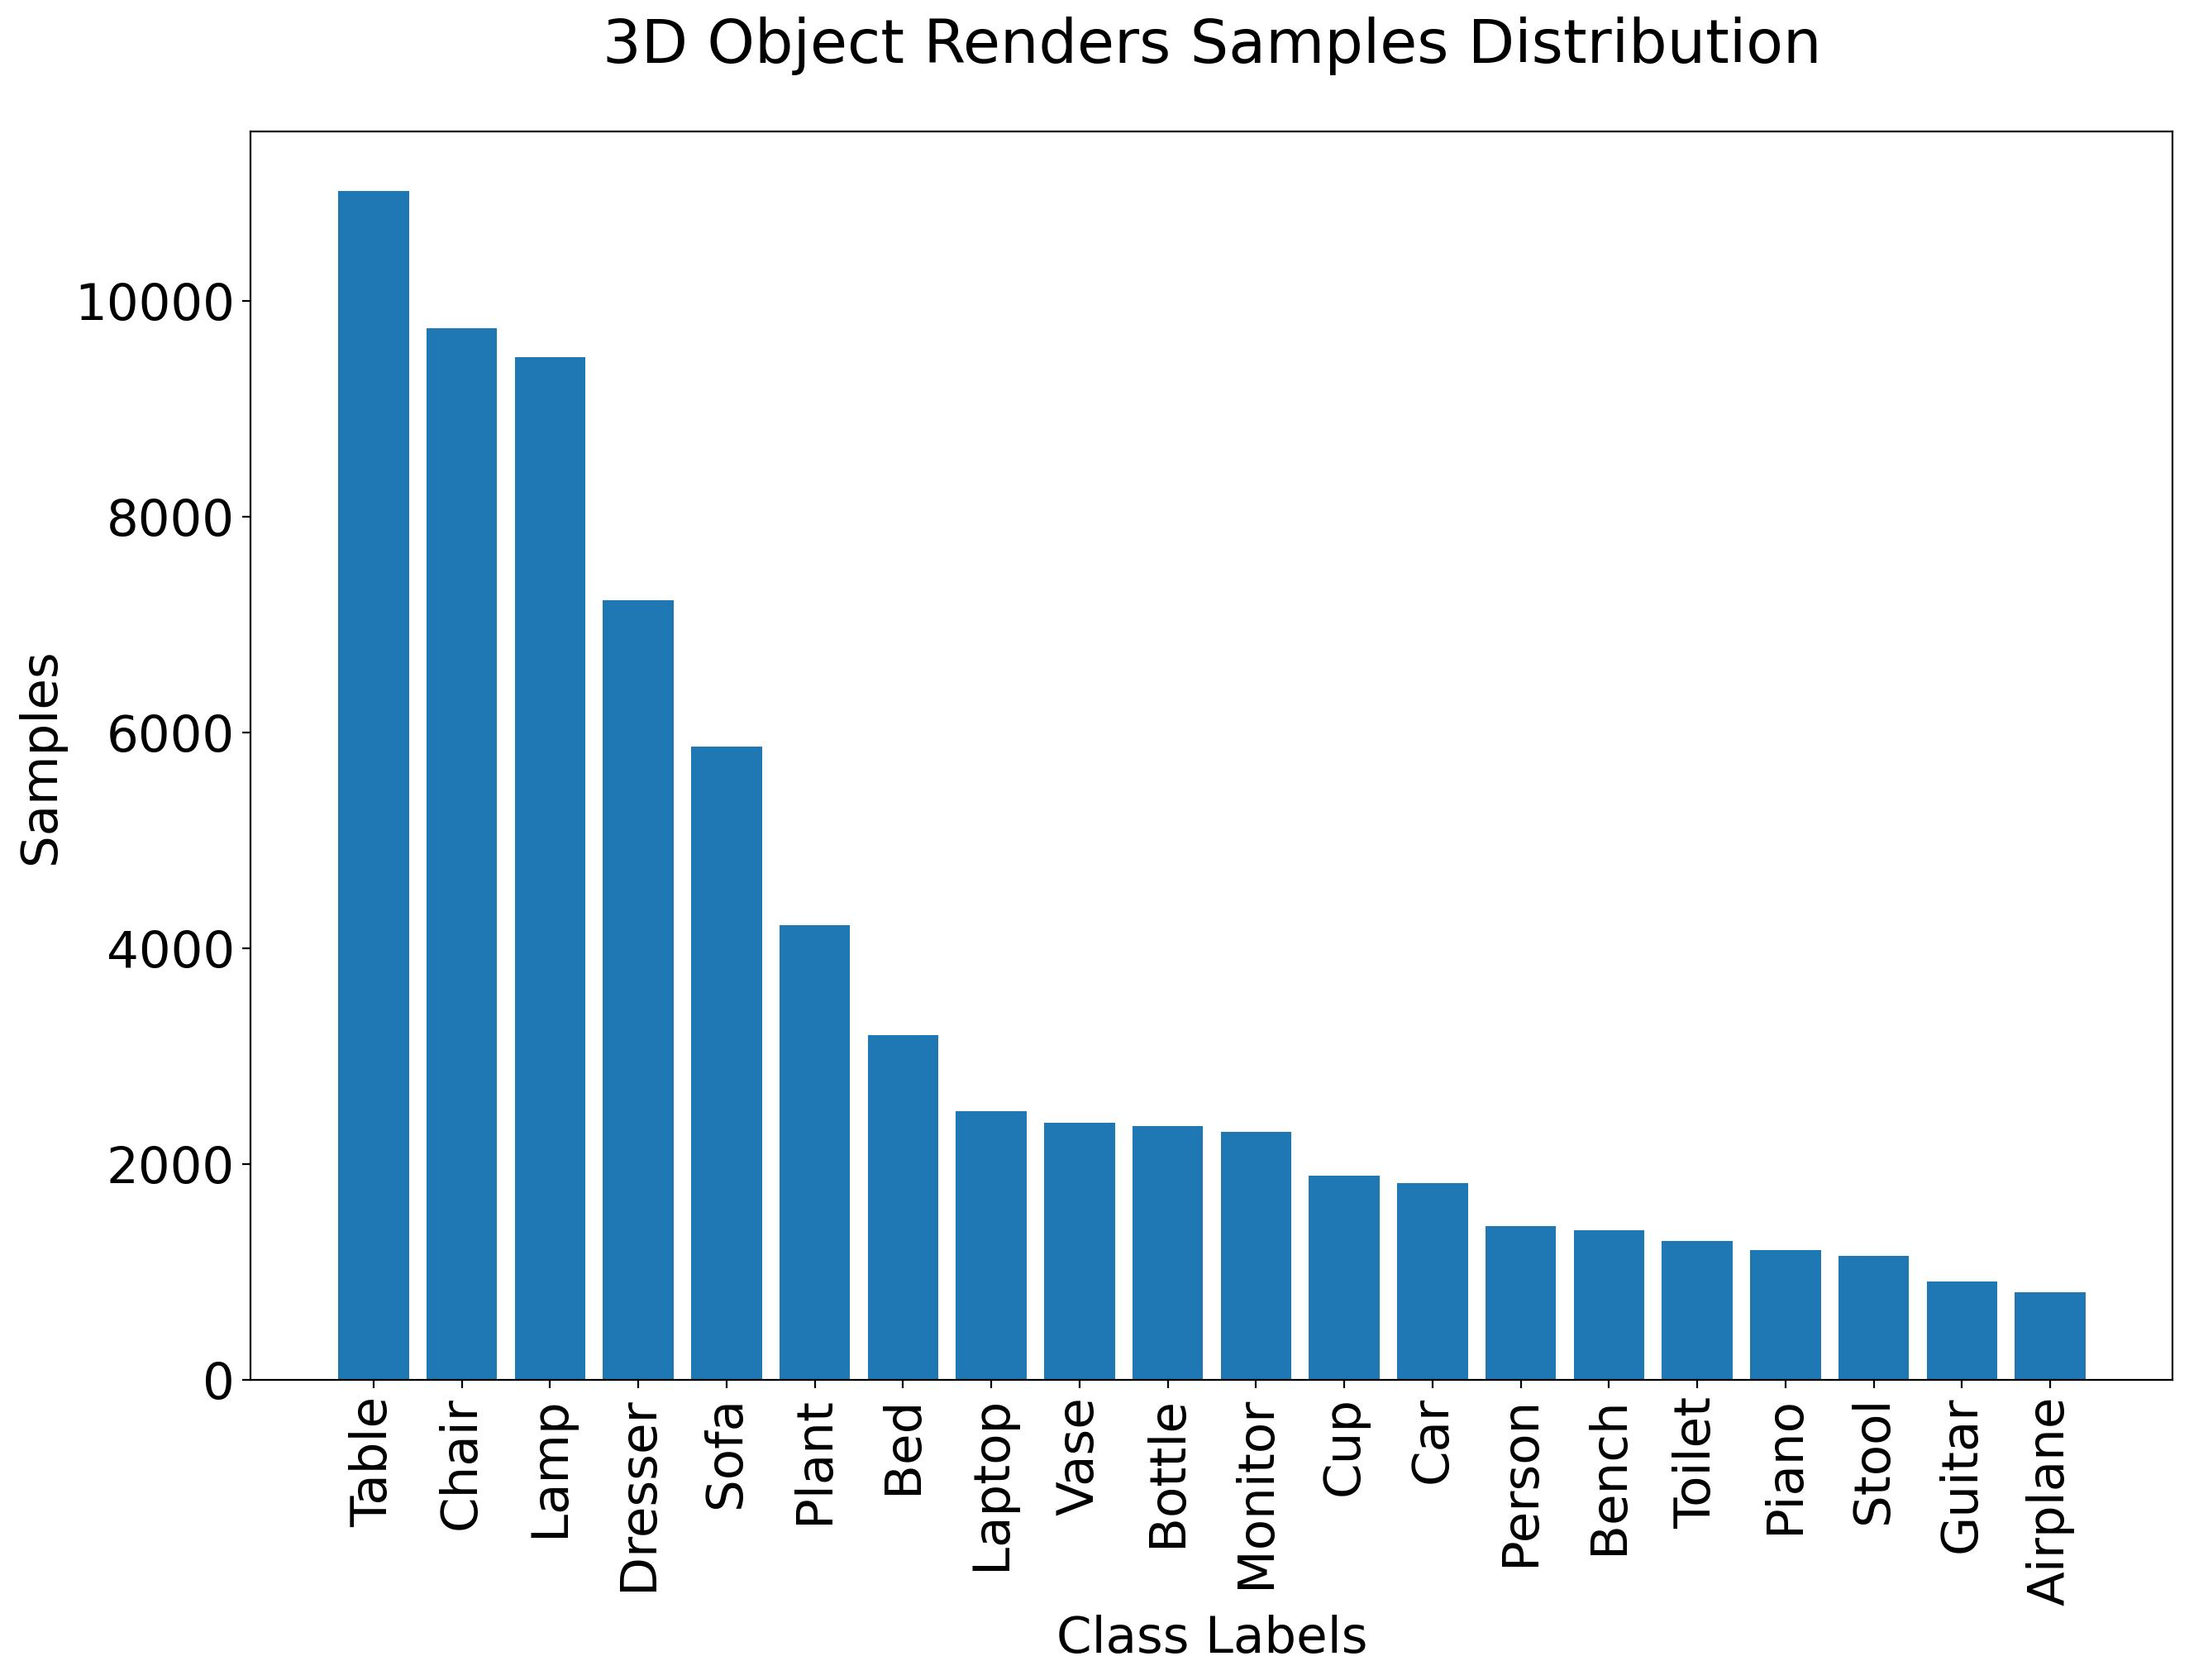
\includegraphics[scale=0.35]{imgs/3d-object-renders-samples-distribution.jpg}
    \caption{RGB Images (3D Objects Renders) Samples per class}
\end{figure}
\noindent
In this case, undersampling was not an option since this would mean loosing almost $85\%$ of the samples of the majority class. Instead, the choice was made to use \textbf{oversampling}. The ModelNet\cite{wu20153d} dataset\footnote{\url{https://modelnet.cs.princeton.edu/}} was used to augment 3D objects.\\
After oversampling, this is the final result obtained:
\begin{figure}[H]
    \centering
    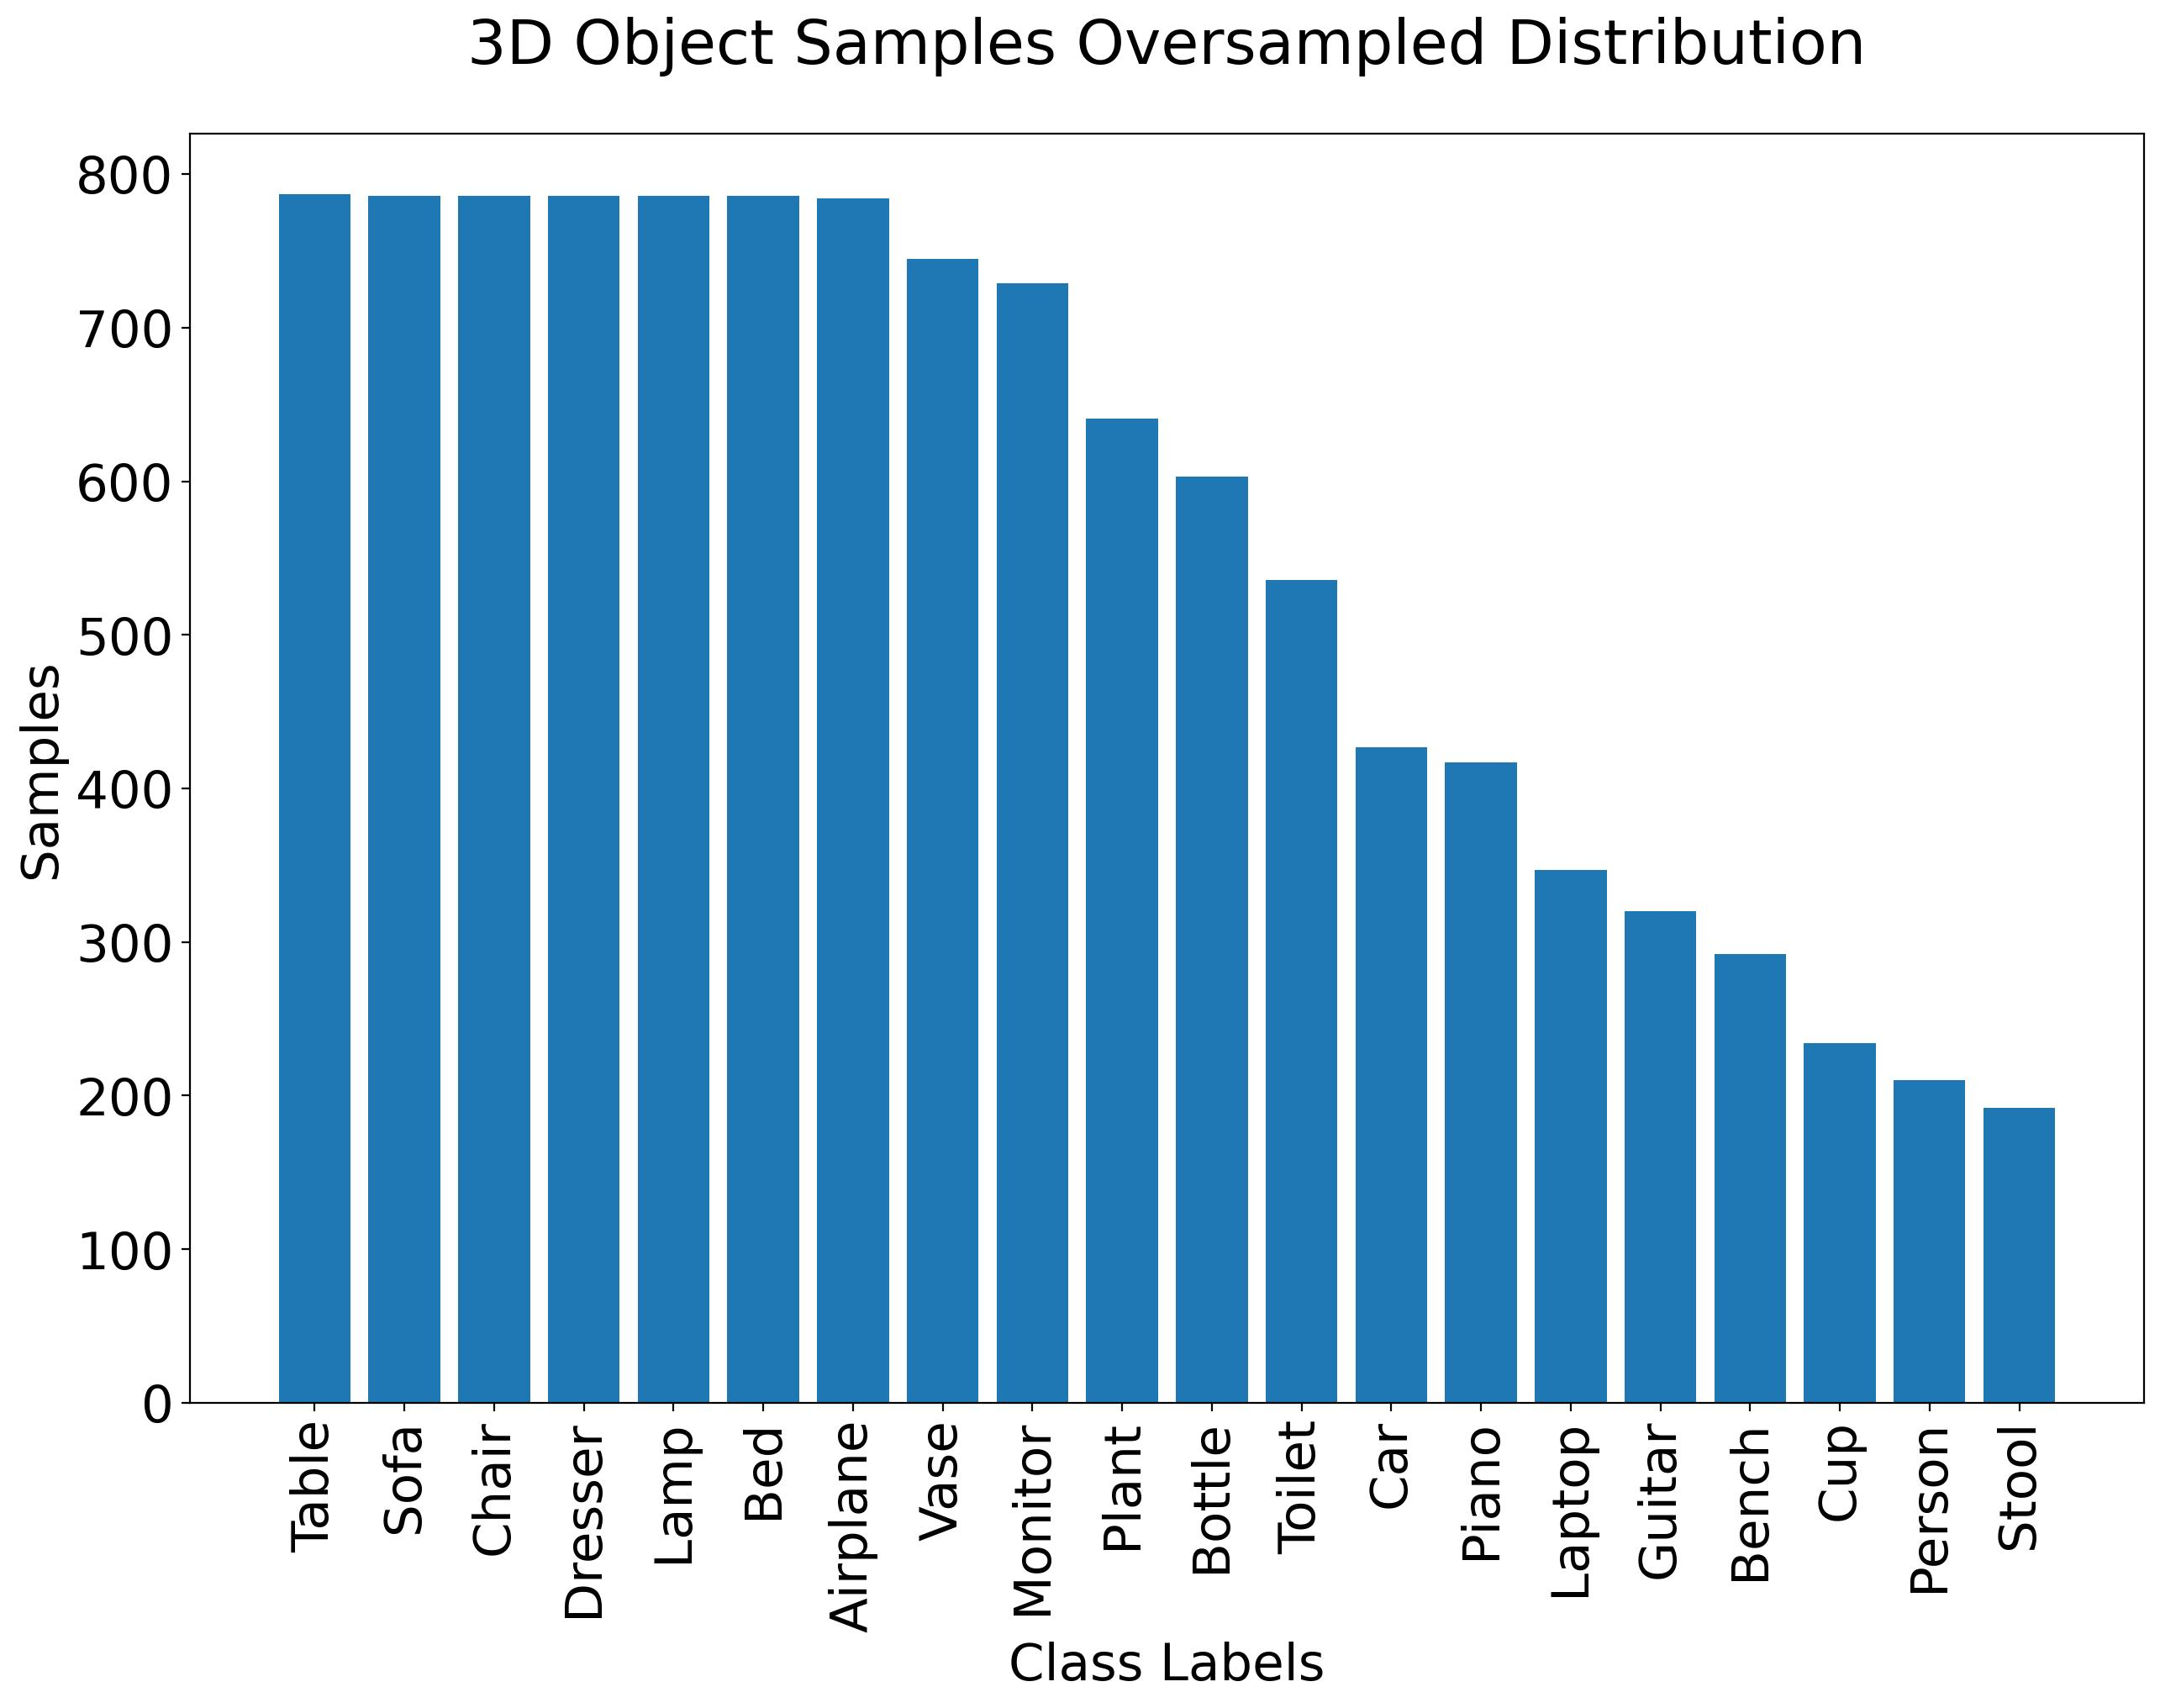
\includegraphics[scale=0.35]{imgs/3d-object-oversampled-distribution.jpg}
    \caption{3D Object Samples per class after oversampling}
\end{figure}
\noindent
A little bit of imbalance is still present, however it \textbf{is not easy to find point cloud data for exactly all the class labels of our interest}.\\
\\
As far as it concerns the RGB images, initially an attempt was made fetching content from
\begin{itemize}
    \item Caltech-101 (\url{http://www.vision.caltech.edu/Image_Datasets/Caltech101}),
    \item Caltech-256 (\url{http://www.vision.caltech.edu/Image_Datasets/Caltech256}),
    \item ImageNet (\url{https://www.image-net.org}),
    \item Open Images Dataset (\url{https://storage.googleapis.com/openimages}),
\end{itemize}
this approach however is limited by two main drawbacks:
\begin{itemize}
    \item the datasets provide images with too much noise (out of context picture with occlusions);
    \item the datasets do not contain the class labels of our interest;
\end{itemize}
As a result, the choice was made to use FastClass\footnote{\url{https://github.com/cwerner/fastclass}}: a tool to crawl search engines (Google, Bing, Baidu, Flickr) and pull all images for a defined set of queries. In addition, files are renamed, scaled and checked for duplicates.\\
After oversampling, this is the final result obtained:
\begin{figure}[H]
    \centering
    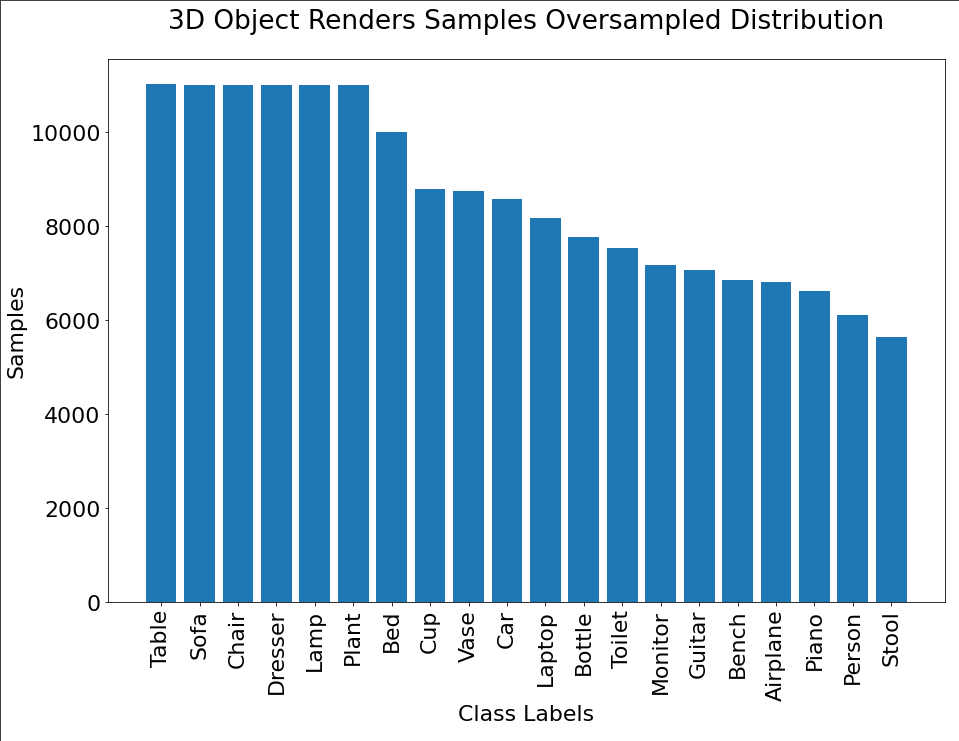
\includegraphics[scale=0.35]{imgs/3d-object-renders-crawling-oversampled-distribution.png}
    \caption{RGB Images (3D Objects Renders) per class after oversampling}
    \label{rgb-images-balancing}
\end{figure}
\noindent
By itself, crawling was not sufficient to fetch enough images to augment the RGB images. This is why I also used image transformations in order to augment the data. To this end, the \texttt{keras.preprocessing.image} package was used.\\
After oversampling, this is the final result obtained:
\begin{figure}[H]
    \centering
    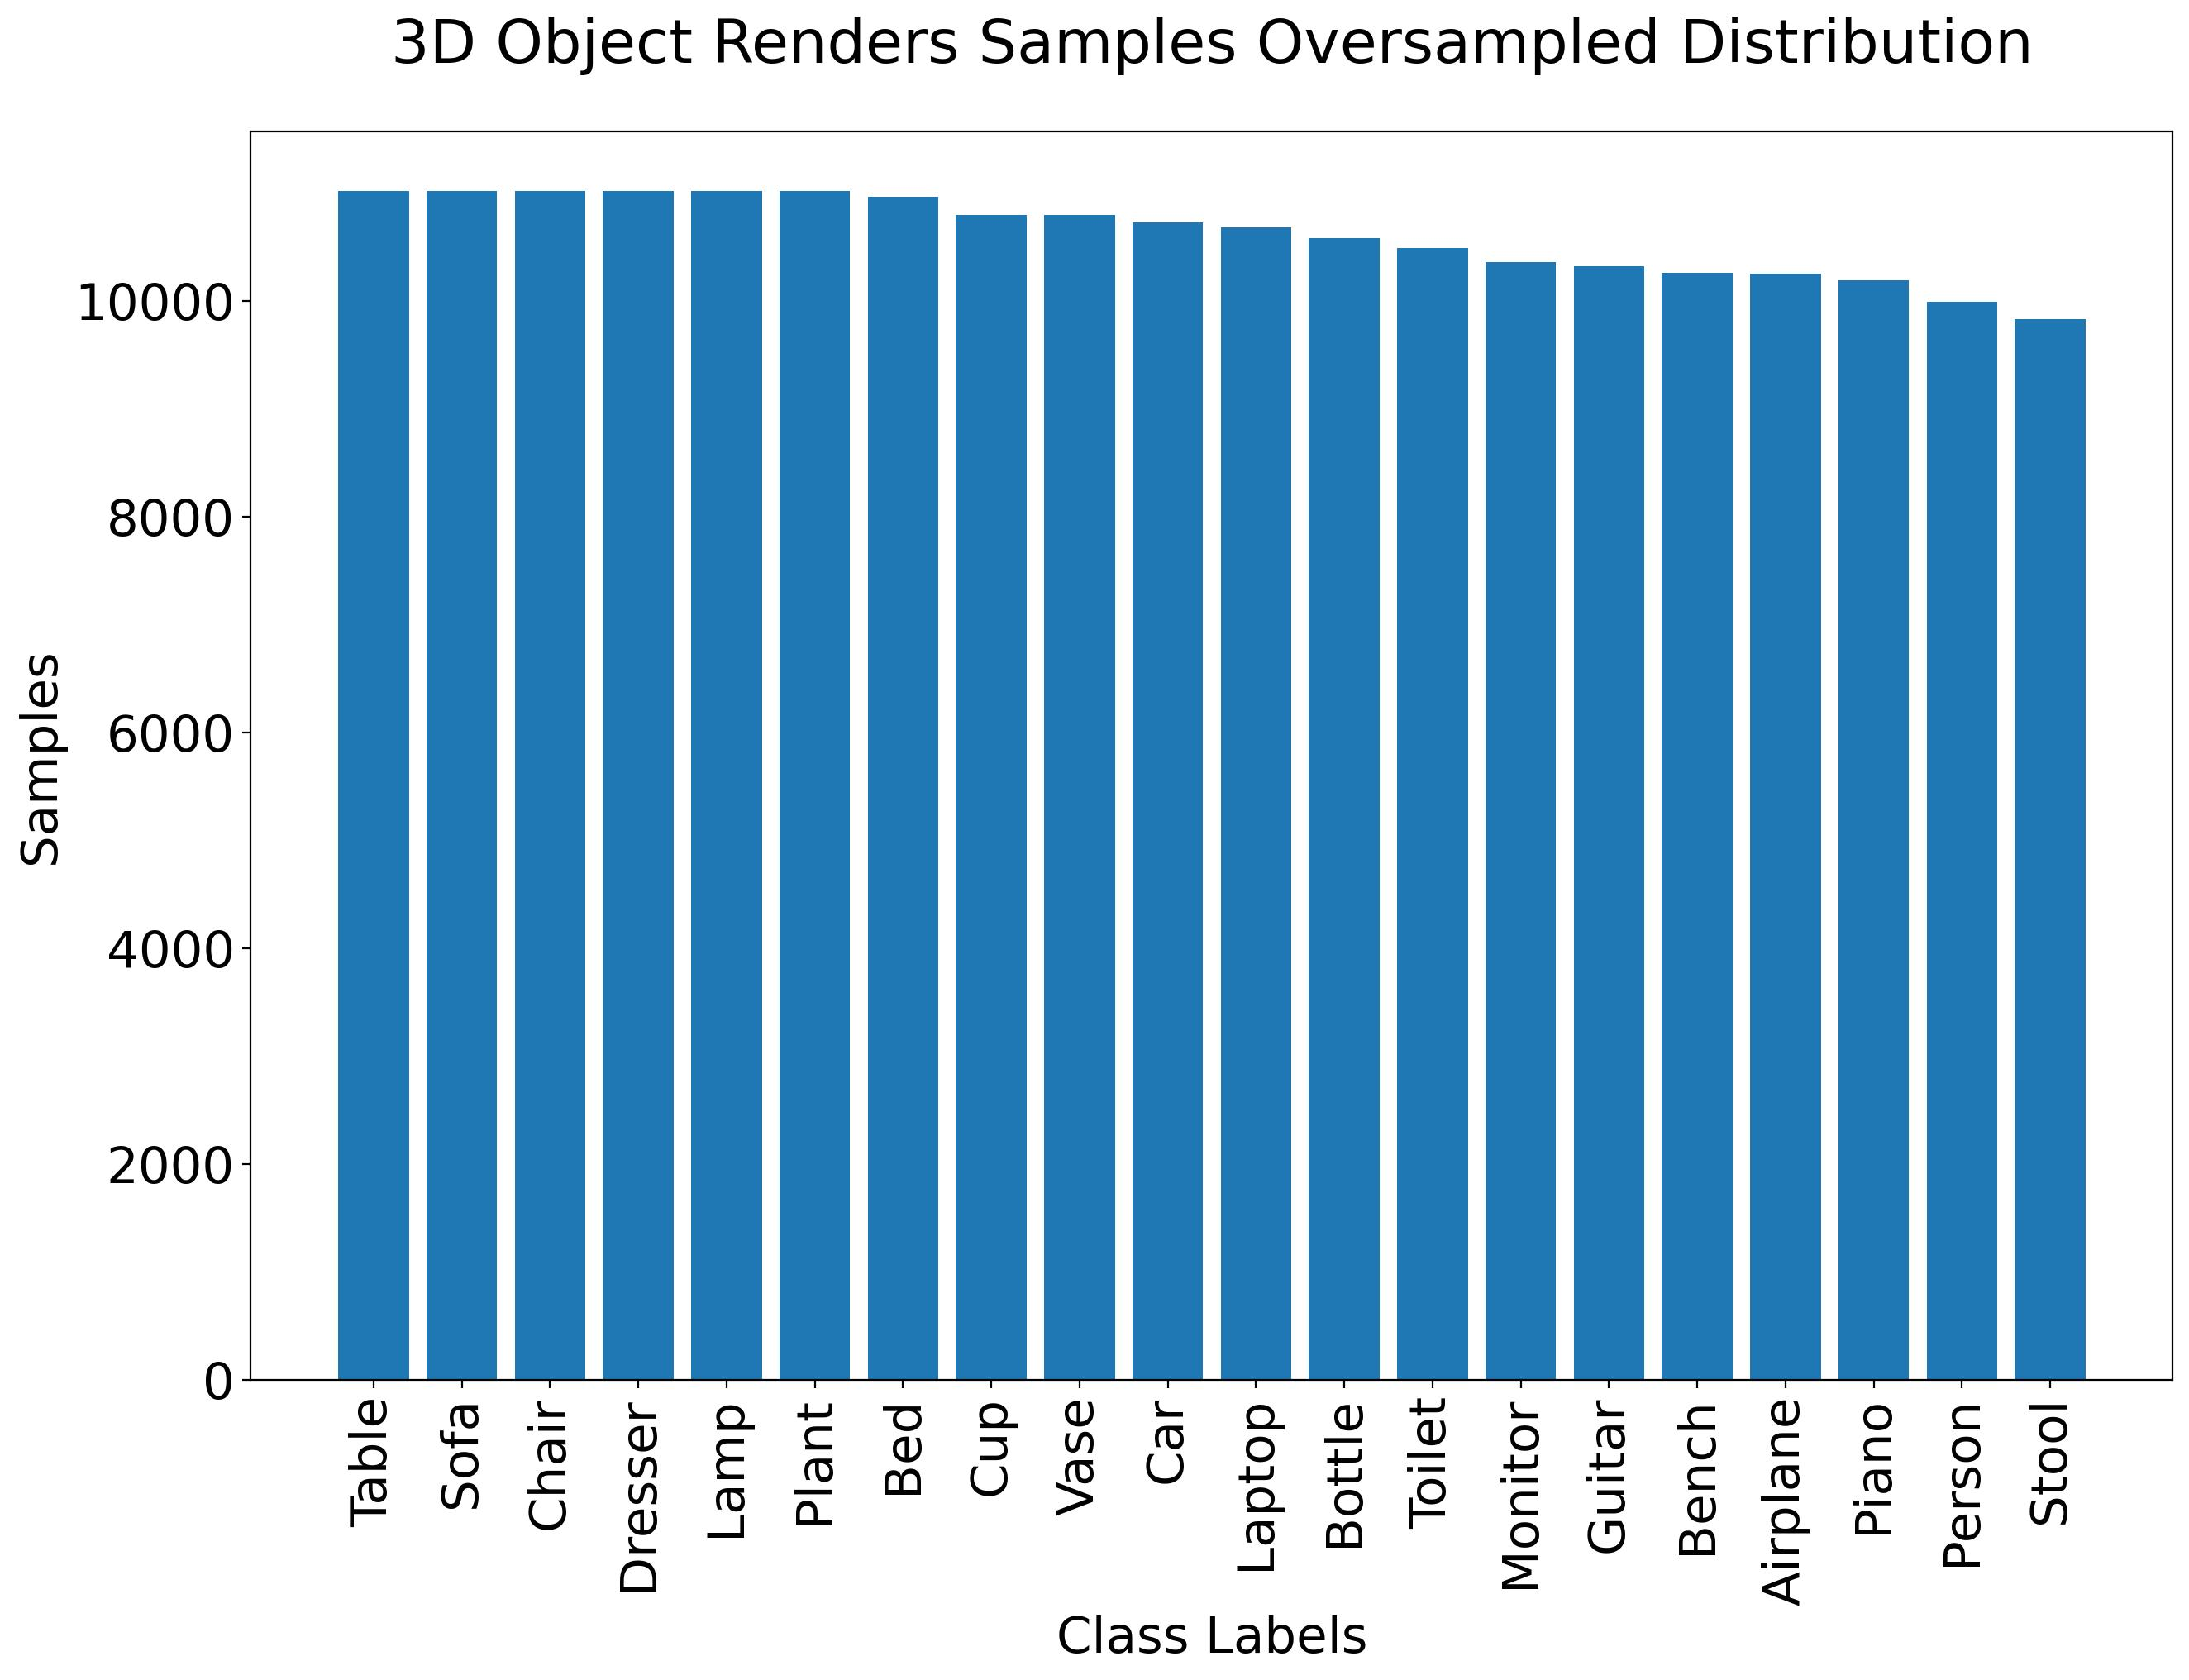
\includegraphics[scale=0.35]{imgs/3d-object-renders-transformations-oversampled-distribution.jpg}
    \caption{RGB Images (3D Objects Renders) per class after oversampling}
\end{figure}
\subsection{Final Class Labels}
Taking into account the entire preprocessing applied to the original dataset, the choice was done to focus the classification task on the top 5 categories of samples: \textbf{Table}, \textbf{Chair}, \textbf{Lamp}, \textbf{Dresser} and \textbf{Sofa}.
\begin{figure}[H]
    \centering
    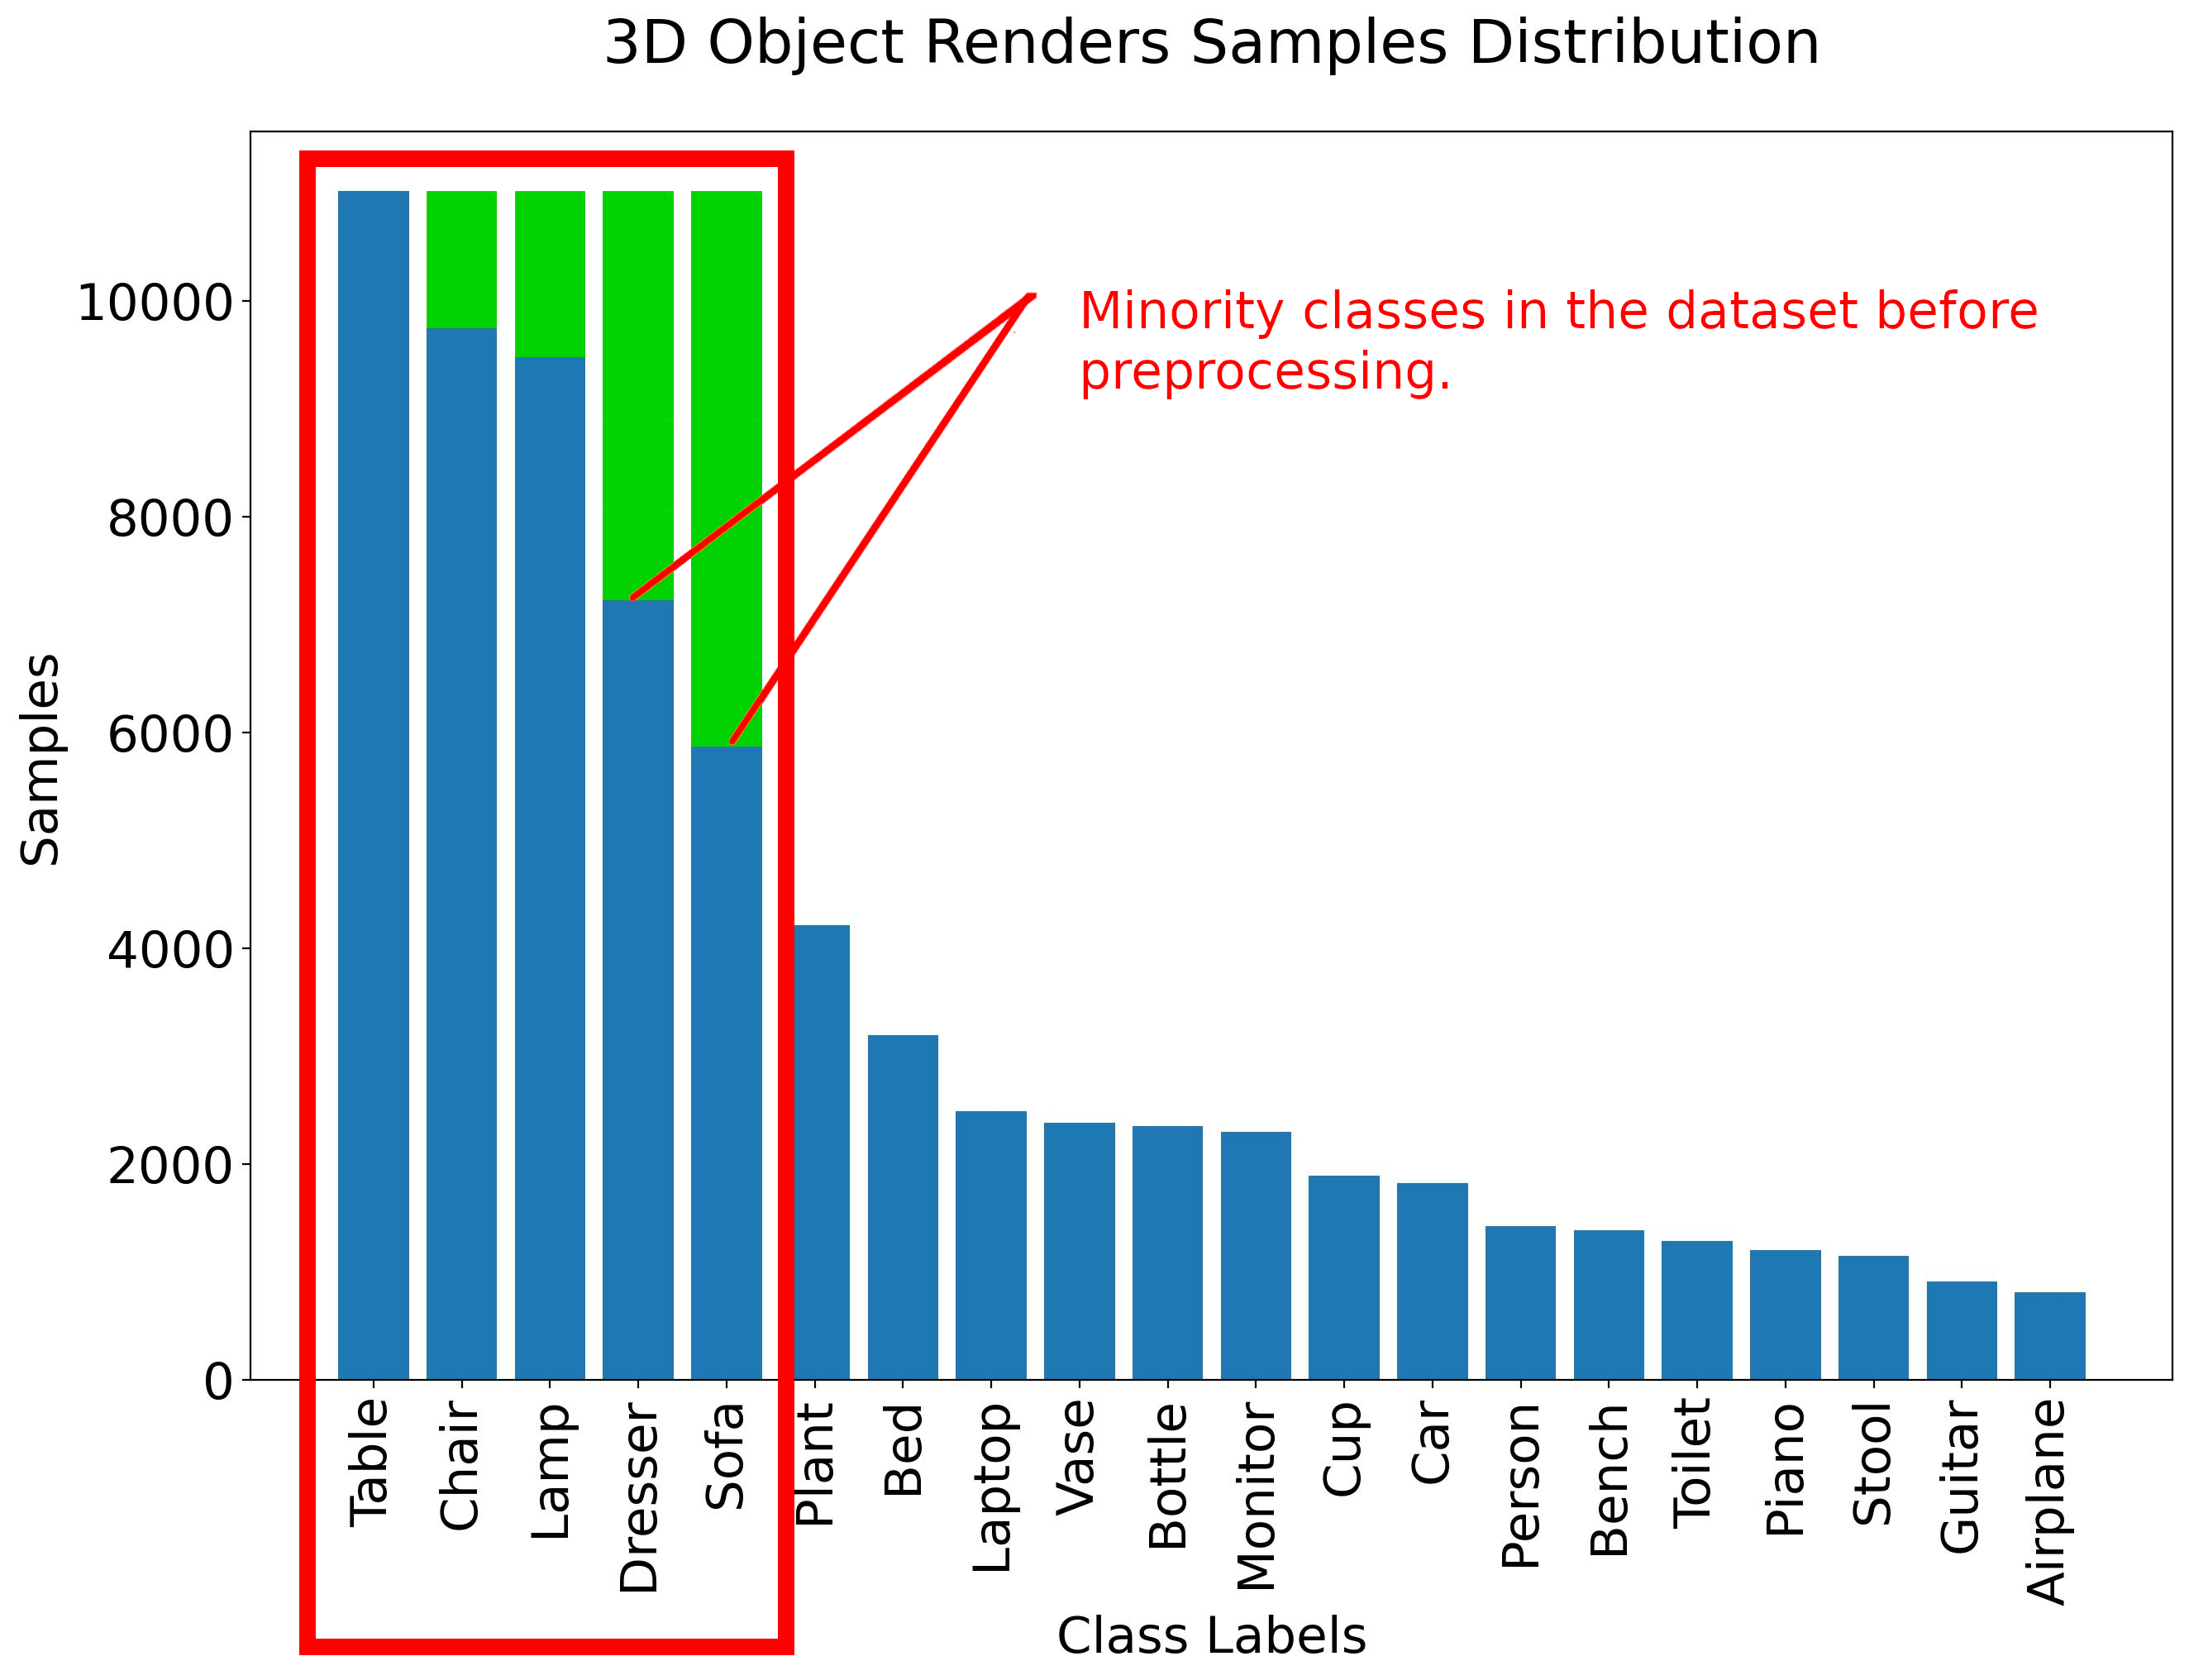
\includegraphics[scale=0.42]{imgs/selected-categories.jpg}
    \caption{Classes of objects for the classification task}
\end{figure}
This choice was made on the basis of the followings:
\begin{itemize}
    \item using too many categories will make the model classification results scores (confusion matrices, ROC curves, etc...) harder to comprehend;
    \item excessive data augmentation was used in order to achieve data balancing for the minor classes which might result in additional noise;
    \item the minority classes \textbf{Dresser} and \textbf{Sofa} were kept in order to be able to later analyse eventual side effects on classification accuracy due to the preprocessing step.
\end{itemize}
\subsection{Stratified K-Fold Cross Validation}
In order to obtain statistically significant results, Stratified K-Fold Cross Validation was implemented. There is no ready made implementation offered by \texttt{tensorflow.keras} that can be used in this case. A custom implementation was made which allows to generate \texttt{train}, \texttt{validation} and \texttt{test}.
\begin{figure}[H]
    \centering
    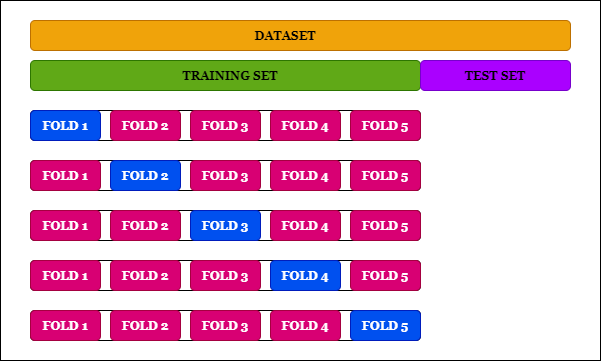
\includegraphics[scale=0.5]{imgs/train-validation-test.png}
\end{figure}
\noindent
The implementation used for the images and for the pointclouds differs since the type of data and the loading procedure are different.
\subsubsection{Stratified K-Fold Cross Validation for images}
\begin{lstlisting}[language=Python,frame=single,caption={Definition of the function used to perform stratified K-Fold cross validation with images data.},captionpos=b]
def images_kfold_validation(model_name, n_splits, test_size, shuffle, layers, learning_rate, decay, target_size, epochs, batch_size, one_fold=True, resample_data=0):
    global images_data
    global images_X
    global images_Y
    if resample_data > 0:
        images_data = images_data.groupby('class_label', group_keys=False).apply(lambda x: x.sample(min(len(x), resample_data), random_state=42))
        images_X = images_data[['filename']]
        images_Y = images_data[['class_label']]

    # fold counter
    fold_counter = 1

    # arrays to store test set loss and accuracy scores for each fold
    TEST_LOSS = []
    TEST_ACCURACY = []

    # split train and test dataset
    images_train, images_test = train_test_split(images_data, test_size=test_size, stratify=images_Y, random_state=42)
    images_train_X = images_train[['filename']]
    images_train_Y = images_train[['class_label']]

    # define stratified k fold cross validation parameters
    stratified_kfold = StratifiedKFold(n_splits=n_splits, random_state=7, shuffle=shuffle)

    # create image generator
    image_data_generator = ImageDataGenerator(width_shift_range=0.1, height_shift_range=0.1, zoom_range=0.3, fill_mode='nearest', horizontal_flip=True, rescale=1./255)

    # test split
    test_data_generator  = image_data_generator.flow_from_dataframe(images_test, directory=None,
                                                        x_col="filename", y_col="class_label",
                                                        class_mode="categorical", shuffle=shuffle,
                                                        target_size=target_size, batch_size=batch_size)

    # generate training and validation folds
    for train_index, validation_index in stratified_kfold.split(images_train_X, images_train_Y):
        print("\n-------- STARTING FOLD: " + str(fold_counter) + " --------")

...
\end{lstlisting}
The most important observations regarding this function include:
\begin{itemize}
    \item it takes as input the model name, layers, and parameters such as the number of folds, the learning rate, the decay rate, the number of epochs and the batch size;
    \item it defines the \texttt{StratifiedKFold} from the \texttt{sklearn.model\_selection} package;
    \item it instantiates the \texttt{ImageDataGenerator} from the \texttt{tf.keras.preprocessing.image} package needed to load the images;
    \item it defines the \texttt{tf.keras.callbacks.ModelCheckpoint} used to save the best model for each fold;
    \item it first generates the \textbf{test} and \textbf{train} folds; the train fold is then used to generate train and \textbf{validation} folds;
    \item it compiles the \texttt{tf.keras} model using the given layers;
    \item it trains and test the model plotting:
    \begin{itemize}
        \item train and validations sets accuracy and loss;
        \item confusion matrix computed on the test set;
    \end{itemize}
    \item new data generators are created in each iteration as the training data and the validation data changes;
    \item if specified, it perform sampling on the dataset in order to reduce the numerosity;
    \item it allows to perform "one fold" training; this was used for the initial experimental models in order to avoid to waste too much time;
\end{itemize}
\subsubsection{Stratified K-Fold Cross Validation for pointclouds}
Similarly, a utility function was written also for handling stratified K-Fold cross validation with pointclouds. The main difference between the two is how the data is loaded and some initialization parameters:
\begin{lstlisting}[language=Python,frame=single,caption={Snippet of the function used to perform stratified K-Fold cross validation with pointclouds data showing how samples are loaded using trimesh.},captionpos=b]
    # split train and test dataset
    pointclouds_train, pointclouds_test = train_test_split(pointclouds_data, test_size=test_size, stratify=pointclouds_Y, random_state=42)
    pointclouds_train_X = pointclouds_train[['filename']]
    pointclouds_train_Y = pointclouds_train[['class_label']]

    # define stratified k fold cross validation parameters
    stratified_kfold = StratifiedKFold(n_splits=n_splits, random_state=7, shuffle=shuffle)

    # test data arrays
    test_pointclouds = []
    test_labels = []
    test_string_labels = {}

    # test split ready
    for index, test_data_row in pointclouds_test.iterrows():
        test_pointclouds.append(trimesh.load(test_data_row['filename'], force='mesh').sample(target_size))
        test_labels.append(class_labels_dict[test_data_row['class_label']])
        test_string_labels[index] = test_data_row['class_label']
    
    # convert to numpy array
    test_pointclouds = numpy.array(test_pointclouds)
    test_labels = numpy.array(test_labels)

    # create test tf.data.Dataset
    test_dataset = tensorflow.data.Dataset.from_tensor_slices((test_pointclouds, test_labels))
    test_dataset = test_dataset.shuffle(len(test_pointclouds)).batch(batch_size)
    print("Found " + str(len(pointclouds_test)) + " validated pointcloud filenames belonging to " + str(len(pointclouds_test['class_label'].unique())) + " classes.")


    # generate train and validation folds
    for train_index, validation_index in stratified_kfold.split(pointclouds_train_X, pointclouds_train_Y):
        print("\n-------- STARTING FOLD: " + str(fold_counter) + " --------")

    ...
\end{lstlisting}
The \texttt{trimesh}\footnote{\url{https://github.com/mikedh/trimesh}} Python package was used in order to work with pointcloud data:
\begin{itemize}
    \item it allows to load both \texttt{.obj} and \texttt{.off} 3D meshes;
    \item is allows to sample pointclouds specifying the number of points;
    \item it allows for pointclouds to be plotted using the \texttt{matplotlib.pyplot} package.
\end{itemize}
For the detailed implementation of the above mentioned functionalities please refer to the Jupyter Notebook named \texttt{KFold-Cross-Validation.ipynb}.

\newpage
\section{Task 2: Training from scratch}
The implementation of what is described in this section can be found in the Jupyter Notebook named \texttt{Task2-Training-from-scratch-images.ipynb} and\\ \texttt{Task2-Training-from-scratch-pointclouds.ipynb}.\\
\\
This task focused on the development from scratch of an ad-hoc CNN to classify between the selected class labels (\textbf{Table}, \textbf{Chair}, \textbf{Lamp}, \textbf{Dresser} and \textbf{Sofa}) using both RGB images and 3D point clouds.\\
\\
In practice, applied Machine Learning is a highly iterative process. As a matter of fact, while our \textit{trainable parameters} (the weights) are obtained as a result of the training procedure, the hyperparameters must be provided as input to the training process. Even very experienced Deep Learning practitioners fail to get hyperparameters right the first time. The process is to turn the idea into code, experiment, and evaluate the outcome and make changes and repeat the process until you get the expected or otherwise a satisfactory outcome. In simpler words it is a trial and error process which can sometimes be helped by guidance found in the literature.\\
\\
In what follows, this trial and error process is described. Each of the following subsections is dedicated to one experiment and the results obtained. Starting from the obtained results, a new experiment is proposed and tested:
\begin{itemize}
    \item the same network was trained and tested on both RGB images and pointclouds, of course the input layers are different given the different nature of the input data;
    \item Stratified K-Fold Cross Validation was used in order to generate \texttt{train}, \texttt{validation} and \texttt{test} sets; the \texttt{train} set was used to perform the training, the performance on the \texttt{validation} set was used in order to tune hyperparameters and the generalization capability of the model is shown by the performance on the \texttt{test} set;
    \item each model was trained for \texttt{100} epochs; the model with the lowest \texttt{validation loss} during the entire training process is saved as \texttt{best model}; the \texttt{best model} is tested on the test set;
    \item the initial experiments focused on tuning the \texttt{capacity} of the model; as soon as \texttt{overfitting} behavior is spotted, \texttt{regularization} techniques will be used to fight back;
    \item Stratified K-Fold Cross Validation was used with \texttt{K = 6}; only the results of the fold with the lowest (pessimistic approach) scores are reported, for the results of the remaining folds please refer to the Jupyter Notebook \texttt{Task2-Training-from-scratch.ipynb};
    \item models for RGB images were trained using the \texttt{RMSprop} optimizer, loss function \texttt{categorical\_crossentropy} and \texttt{accuracy} metric;
    \item models for 3D pointclouds were trained using the \texttt{RMSprop} optimizer, loss function \texttt{sparse\_categorical\_crossentropy} and \texttt{sparse\_categorical\_accuracy} metric;
\end{itemize}
\subsection{RGB Images}
The experiments performed on the dataset of RGB images are now presented.
\subsubsection{Experiment 0 - Simple Model}
The best place where to start is with the simplest model possible, so simple that we can consider it a naive experiment. At this stage, we are mainly focused in finding the \textit{capacity} of our model, that is the number of hidden layers and number of hidden units per hidden layer to be used in our CNN.\\
The model is made of $2$ convolutional layers interleaved with max-pooling, and after a fully connected layer with $32$ units, the output layer is obtained using $5$ neurons with \texttt{softmax} activation:
\begin{lstlisting}[language=bash,frame=single]
# experiment model layers
layers = [
    Conv2D(32, (3, 3), activation='relu', input_shape=(64, 64, 3)),
    MaxPooling2D(pool_size=(2, 2)),
    Conv2D(64, (3, 3), activation='relu'),
    MaxPooling2D(pool_size=(2, 2)),
    Flatten(),
    Dense(32),
    Activation('relu'),
    Dense(NUM_CLASSES, activation='softmax')
]

# train, validate and test
images_kfold_validation(model_name="Experiment-0", n_splits=2, test_size=0.10,
                        shuffle=True, layers=layers, learning_rate=0.001,
                        decay=1e-6, target_size=(32, 32), epochs=50,
                        batch_size=32, one_fold=True, resample_data=3000)
\end{lstlisting}
Default training hyperparameters (\texttt{learning rate}, \texttt{decay}, etc...) of \texttt{RMSprop} implementation were used. Contrary to what I expected, this simple model \textbf{overfitted} the dataset with more than $12,000$ samples quite rapidly.
\begin{figure}[H]
    \centering
    \subfloat[\centering 3D Object]{{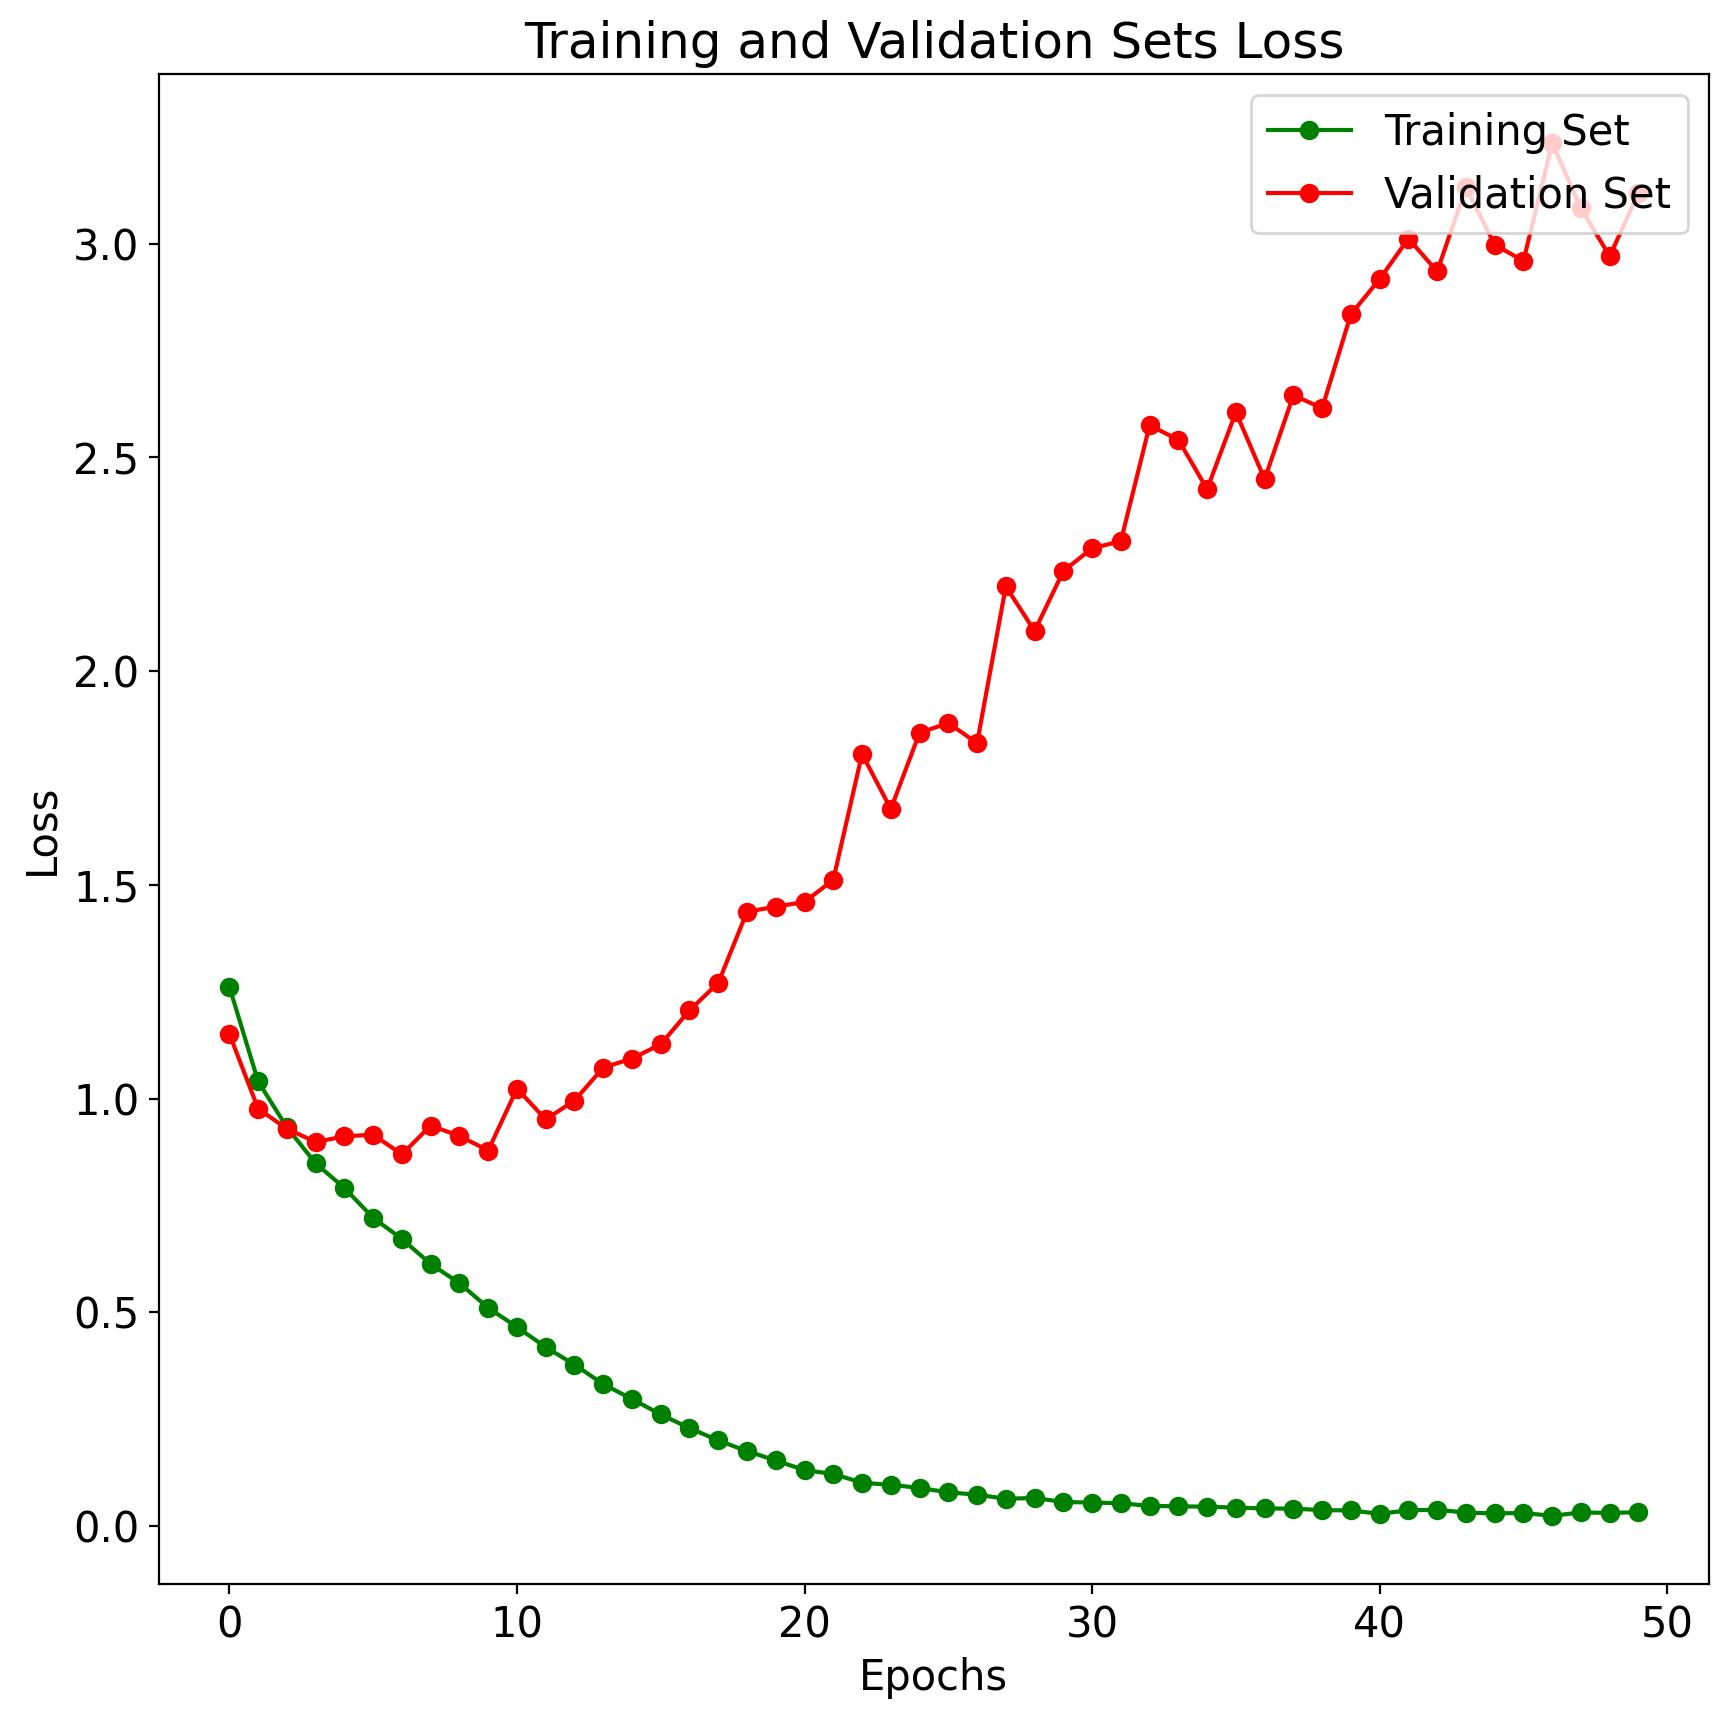
\includegraphics[scale=0.31]{imgs/experiments/images/0/Experiment-0-fold-1.h5-train-val-loss.jpg} }}
    \qquad
    \subfloat[\centering Sampled Point Cloud]{{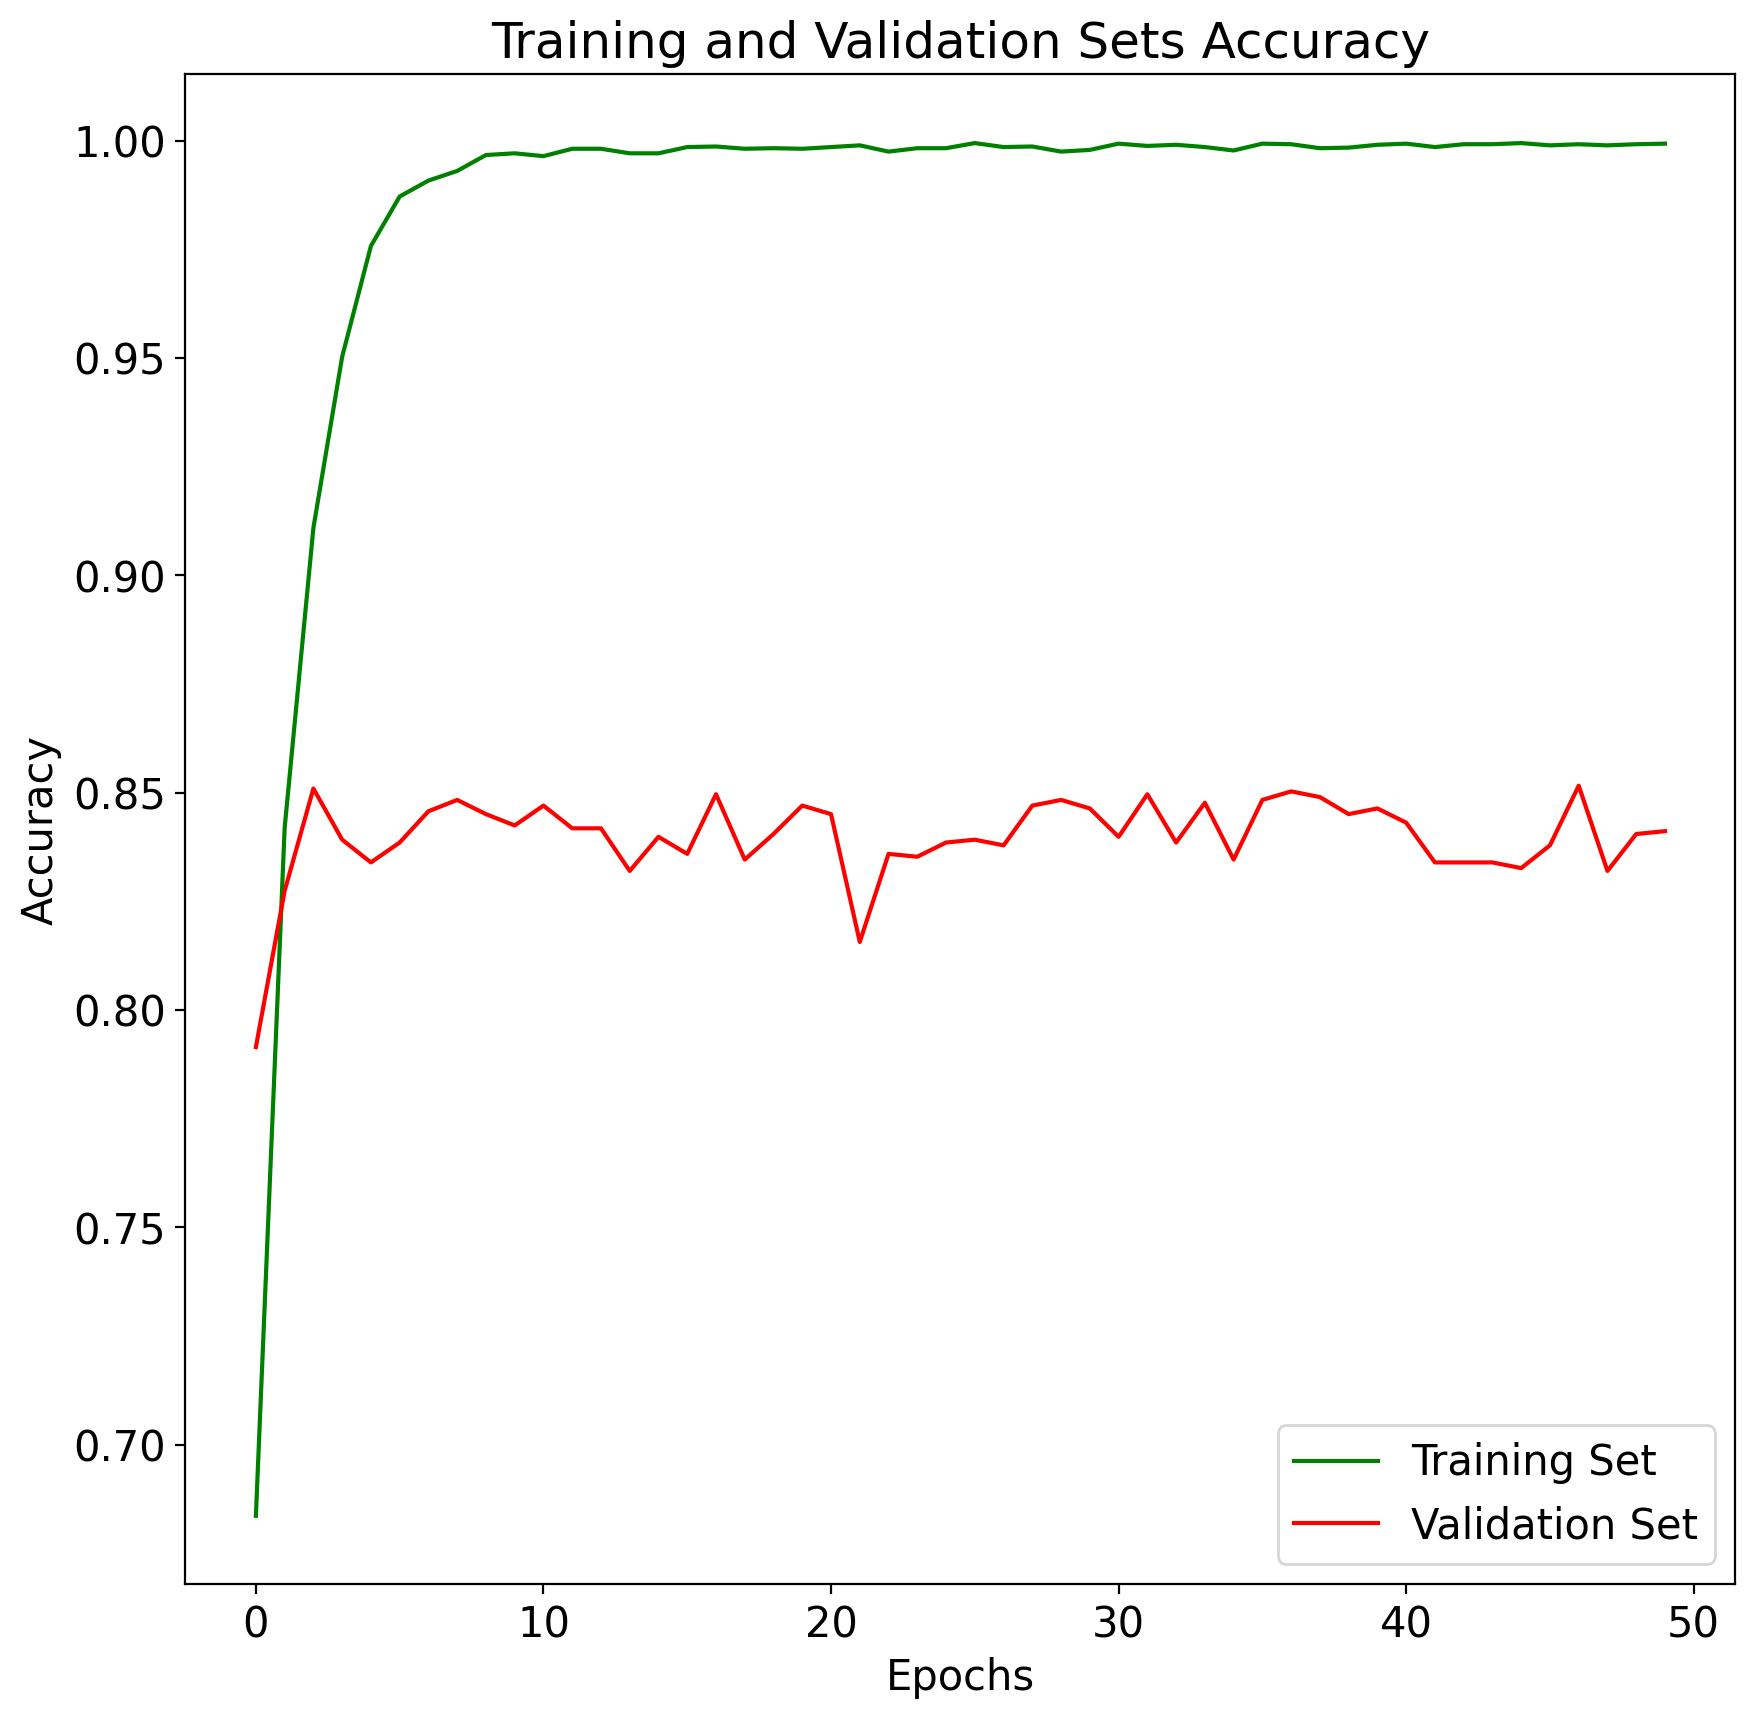
\includegraphics[scale=0.31]{imgs/experiments/images/0/Experiment-0-fold-1.h5-train-val-accuracy.jpg} }}
    \caption{Experiment 0 Results}
\end{figure}
\noindent
\subsubsection{Experiment 1 - Model}
\subsubsection{Experiment 2 - Model}
\subsubsection{Experiment 3 - Model}
\subsubsection{Experiment 4 - Model}
\subsection{3D Pointclouds}
The experiments performed on the dataset of pointclouds are now presented. Before moving on, I would like to clarify that most of the inspiration for the work that follows was taken from external papers and articles:
\begin{itemize}
    \item PointNet: Deep Learning on Point Sets for 3D Classification and Segmentation\cite{qi2017pointnet};
    \item An In-Depth Look at PointNet\cite{mediumcompointnet};
    \item Deep learning with point clouds\cite{romainthalineaupointclouds}.
    \item \textbf{never the less, the implementation code is mine and no ready made source code was used.}
\end{itemize}
\subsubsection{Experiment 0 - Naive Model}
I voluntarily performed this experiment which is intended to demonstrate some of the limitations of traditional ConvNets to handle pointcloud data. The model is the same as the one tested in \texttt{Experiment 0 - Simple Model} on RGB images made of $2$ convolutional layers interleaved with max-pooling, a fully connected layer with $32$ units, and the output layer obtained using $5$ neurons with \texttt{softmax} activation:
\begin{lstlisting}[language=bash,frame=single]
layers = [
    Conv2D(32, (3, 3), activation='relu', input_shape=(64, 64, 3)),
    MaxPooling2D(pool_size=(2, 2)),
    Conv2D(64, (3, 3), activation='relu'),
    MaxPooling2D(pool_size=(2, 2)),
    Flatten(),
    Dense(32),
    Activation('relu'),
    Dense(NUM_CLASSES, activation='softmax')
]
\end{lstlisting}
\begin{figure}[H]
    \centering
    \subfloat[\centering 3D Object]{{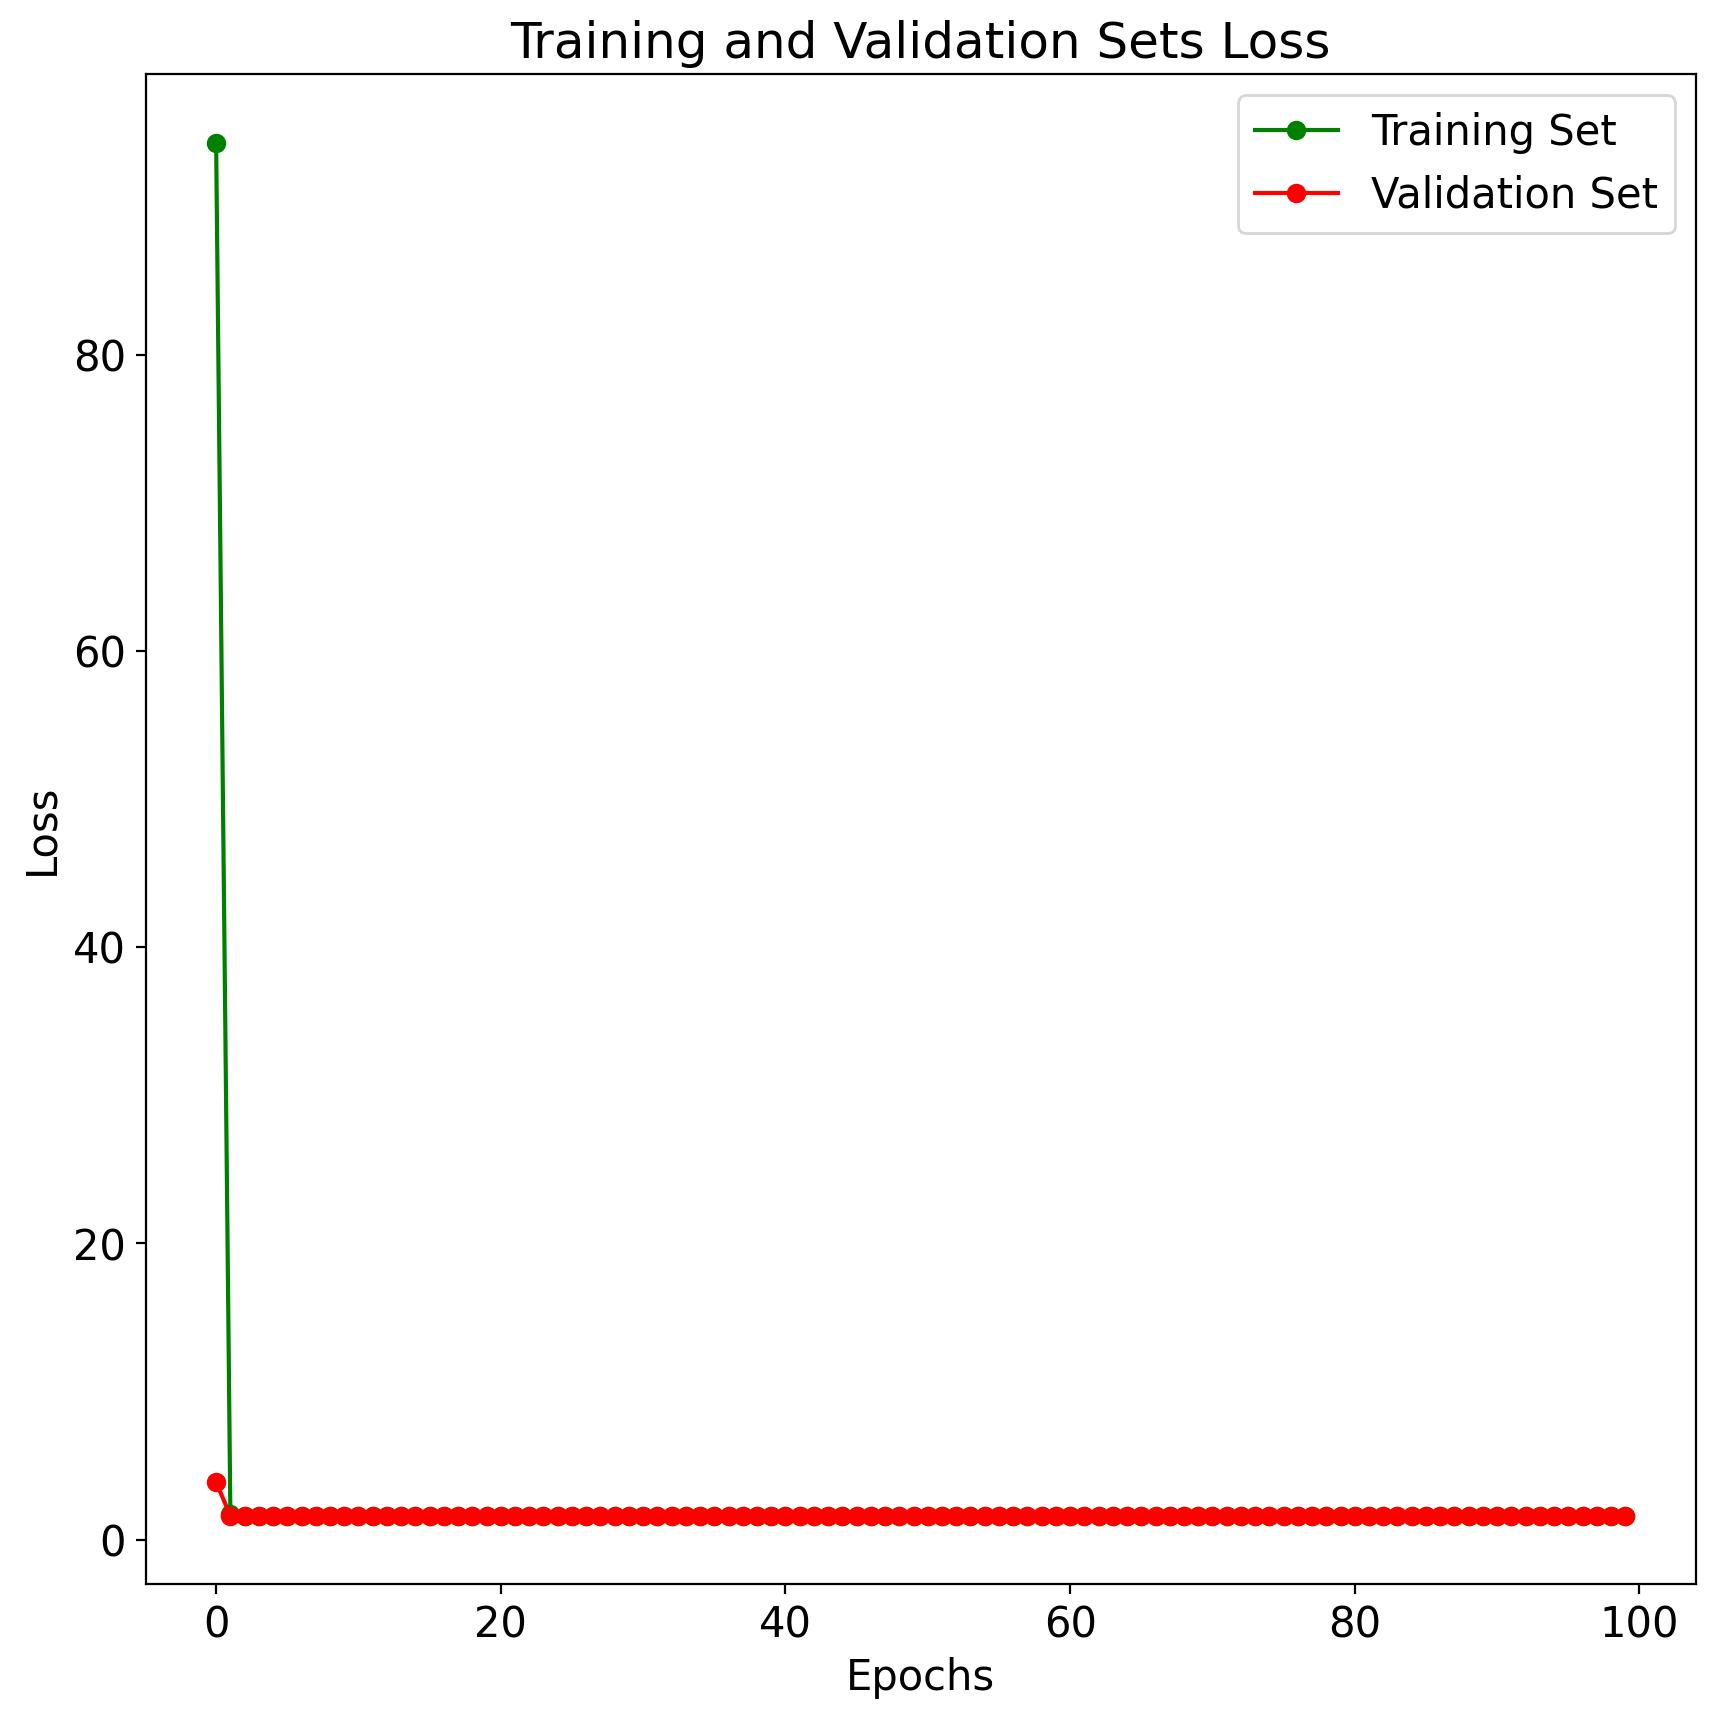
\includegraphics[scale=0.3]{imgs/experiments/pointclouds/0/Experiment-0-fold-1.h5-train-val-loss.jpg} }}
    \qquad
    \subfloat[\centering Sampled Point Cloud]{{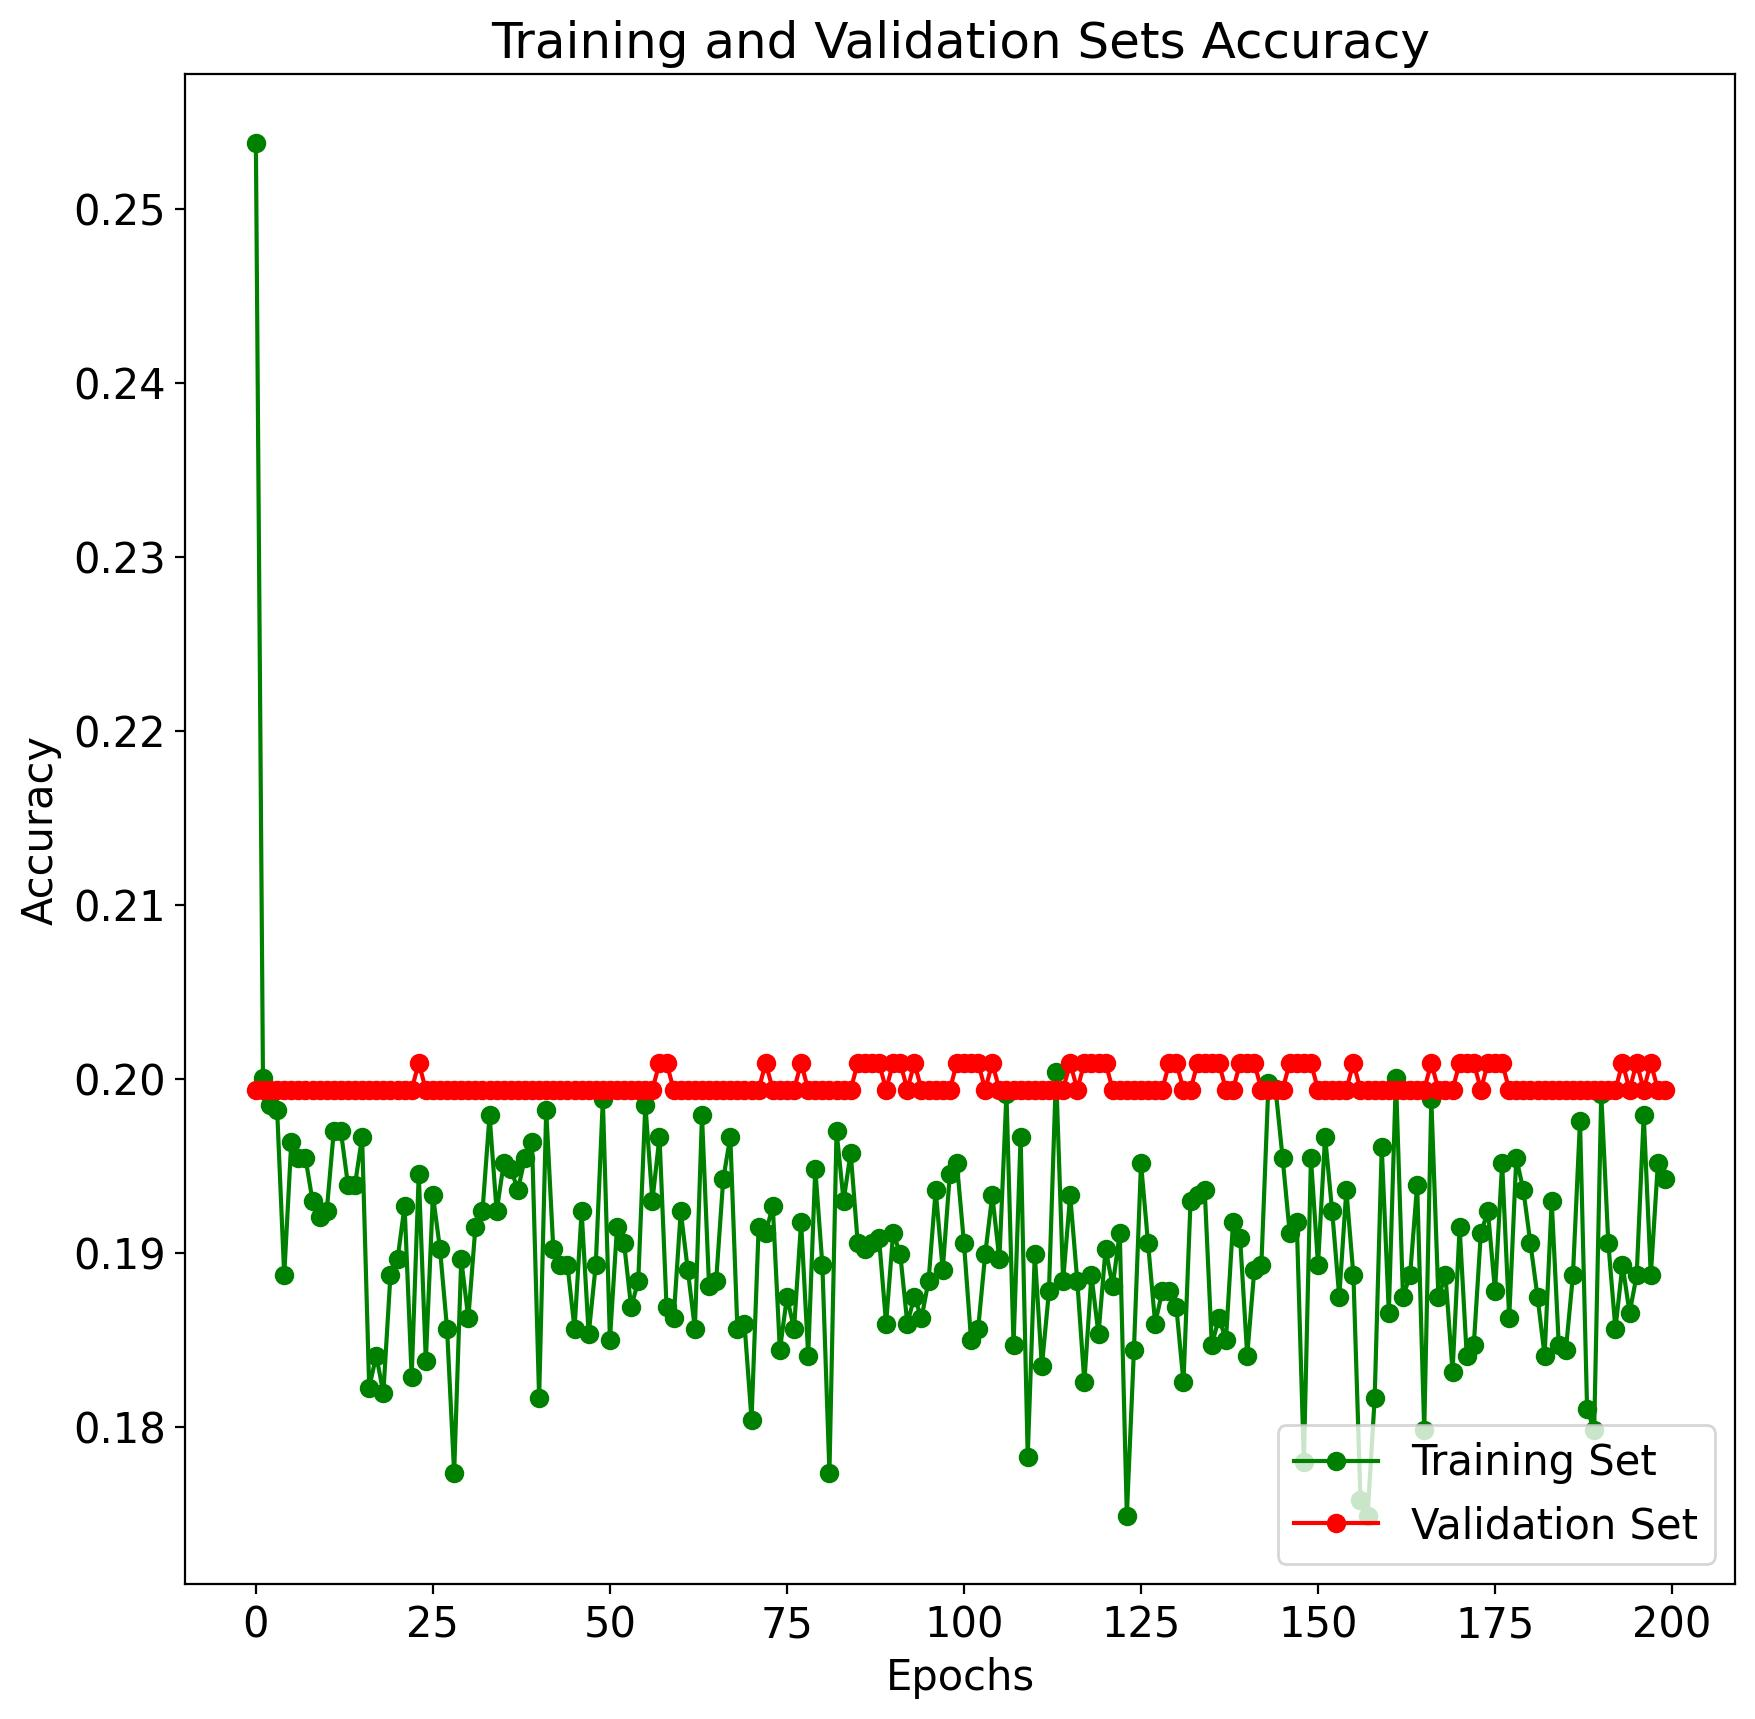
\includegraphics[scale=0.3]{imgs/experiments/pointclouds/0/Experiment-0-fold-1.h5-train-val-accuracy.jpg} }}
    \caption{Experiment 0 Results}
\end{figure}
In order to explain the results obtained, let's make a step back. As previously mentioned, the convolution operation is one of the key contributors to the 2D vision performance of neural networks. The fundamental building block of a CNN is illustrated below.
\begin{figure}[H]
    \centering
    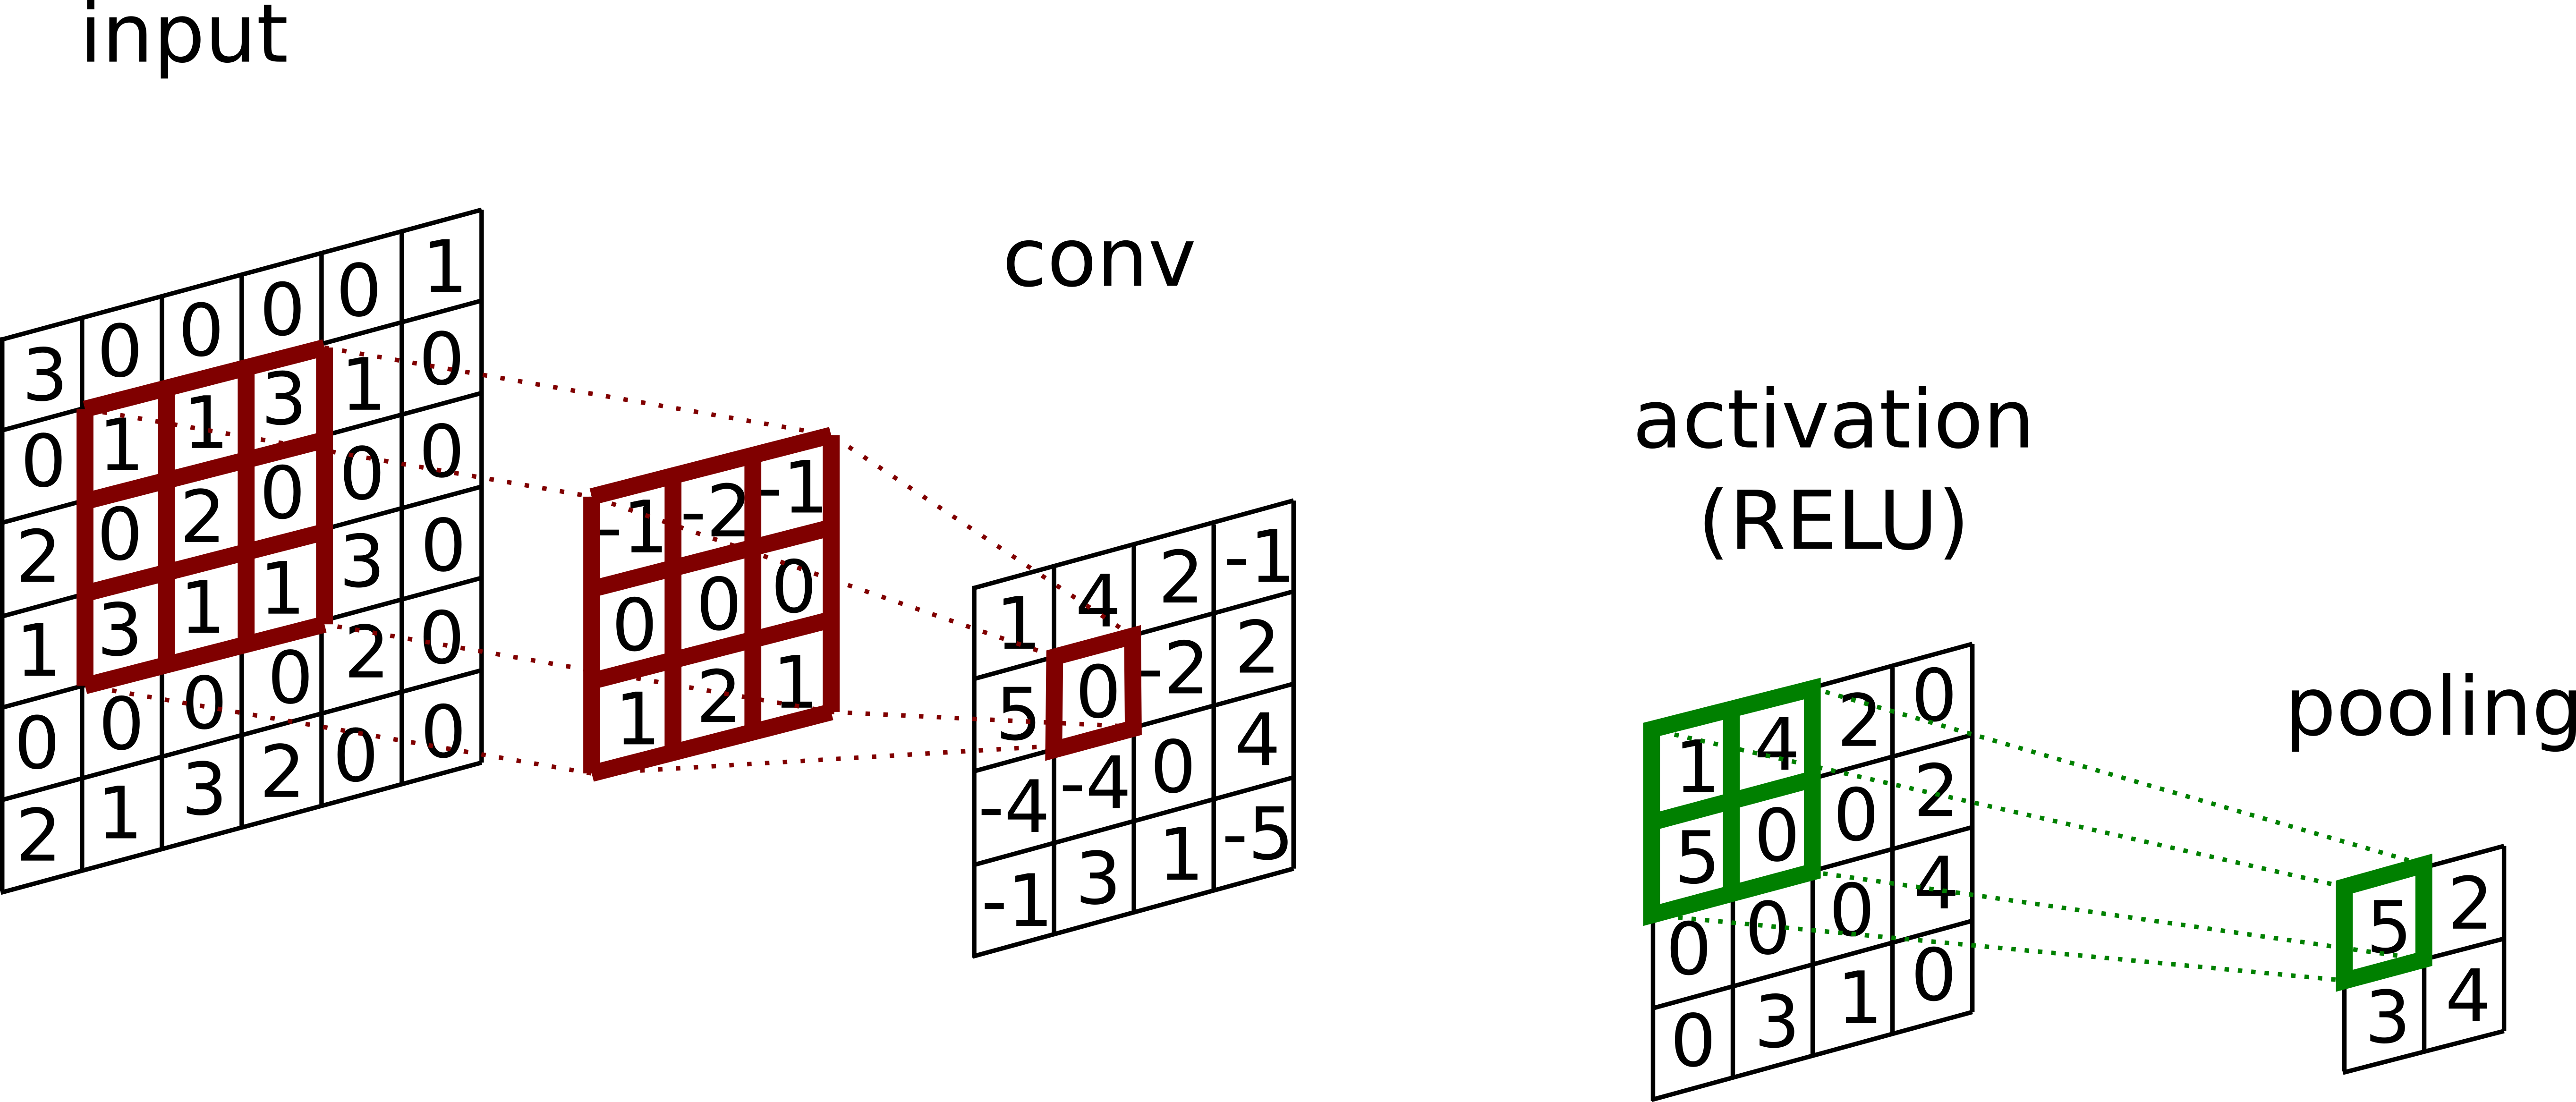
\includegraphics[scale=0.1]{imgs/conv.png}
\end{figure}
\noindent
A kernel is first convolved with the input, then a non linear activation function (e.g. RELU) is applied, and finally a pooling (e.g. max) is performed to produce the so called feature map. Generally there are several kernels applied per block resulting in several feature maps.
\subsubsection{Experiment 1 - Model}
\subsubsection{Experiment 2 - Model}
\subsubsection{Experiment 3 - Model}
\subsubsection{Experiment 4 - Model}

\newpage
\section{Task 3: State-of-the-art}
The implementation of what is described in this section can be found in the Jupyter Notebook named \texttt{Task3-Pre-trained.ipynb}.\\
\\


\newpage
\section{Conclusion}

\newpage
\nocite{kerasiopointnet}
\nocite{mediumcomkfoldcrossvalidation}
\printbibliography
\end{document}